\documentclass[twoside]{book}

% Packages required by doxygen
\usepackage{fixltx2e}
\usepackage{calc}
\usepackage{doxygen}
\usepackage[export]{adjustbox} % also loads graphicx
\usepackage{graphicx}
\usepackage[utf8]{inputenc}
\usepackage{makeidx}
\usepackage{multicol}
\usepackage{multirow}
\PassOptionsToPackage{warn}{textcomp}
\usepackage{textcomp}
\usepackage[nointegrals]{wasysym}
\usepackage[table]{xcolor}

% Font selection
\usepackage[T1]{fontenc}
\usepackage[scaled=.90]{helvet}
\usepackage{courier}
\usepackage{amssymb}
\usepackage{sectsty}
\renewcommand{\familydefault}{\sfdefault}
\allsectionsfont{%
  \fontseries{bc}\selectfont%
  \color{darkgray}%
}
\renewcommand{\DoxyLabelFont}{%
  \fontseries{bc}\selectfont%
  \color{darkgray}%
}
\newcommand{\+}{\discretionary{\mbox{\scriptsize$\hookleftarrow$}}{}{}}

% Page & text layout
\usepackage{geometry}
\geometry{%
  a4paper,%
  top=2.5cm,%
  bottom=2.5cm,%
  left=2.5cm,%
  right=2.5cm%
}
\tolerance=750
\hfuzz=15pt
\hbadness=750
\setlength{\emergencystretch}{15pt}
\setlength{\parindent}{0cm}
\setlength{\parskip}{3ex plus 2ex minus 2ex}
\makeatletter
\renewcommand{\paragraph}{%
  \@startsection{paragraph}{4}{0ex}{-1.0ex}{1.0ex}{%
    \normalfont\normalsize\bfseries\SS@parafont%
  }%
}
\renewcommand{\subparagraph}{%
  \@startsection{subparagraph}{5}{0ex}{-1.0ex}{1.0ex}{%
    \normalfont\normalsize\bfseries\SS@subparafont%
  }%
}
\makeatother

% Headers & footers
\usepackage{fancyhdr}
\pagestyle{fancyplain}
\fancyhead[LE]{\fancyplain{}{\bfseries\thepage}}
\fancyhead[CE]{\fancyplain{}{}}
\fancyhead[RE]{\fancyplain{}{\bfseries\leftmark}}
\fancyhead[LO]{\fancyplain{}{\bfseries\rightmark}}
\fancyhead[CO]{\fancyplain{}{}}
\fancyhead[RO]{\fancyplain{}{\bfseries\thepage}}
\fancyfoot[LE]{\fancyplain{}{}}
\fancyfoot[CE]{\fancyplain{}{}}
\fancyfoot[RE]{\fancyplain{}{\bfseries\scriptsize Generated by Doxygen }}
\fancyfoot[LO]{\fancyplain{}{\bfseries\scriptsize Generated by Doxygen }}
\fancyfoot[CO]{\fancyplain{}{}}
\fancyfoot[RO]{\fancyplain{}{}}
\renewcommand{\footrulewidth}{0.4pt}
\renewcommand{\chaptermark}[1]{%
  \markboth{#1}{}%
}
\renewcommand{\sectionmark}[1]{%
  \markright{\thesection\ #1}%
}

% Indices & bibliography
\usepackage{natbib}
\usepackage[titles]{tocloft}
\setcounter{tocdepth}{3}
\setcounter{secnumdepth}{5}
\makeindex

% Hyperlinks (required, but should be loaded last)
\usepackage{ifpdf}
\ifpdf
  \usepackage[pdftex,pagebackref=true]{hyperref}
\else
  \usepackage[ps2pdf,pagebackref=true]{hyperref}
\fi
\hypersetup{%
  colorlinks=true,%
  linkcolor=blue,%
  citecolor=blue,%
  unicode%
}

% Custom commands
\newcommand{\clearemptydoublepage}{%
  \newpage{\pagestyle{empty}\cleardoublepage}%
}

\usepackage{caption}
\captionsetup{labelsep=space,justification=centering,font={bf},singlelinecheck=off,skip=4pt,position=top}

%===== C O N T E N T S =====

\begin{document}

% Titlepage & ToC
\hypersetup{pageanchor=false,
             bookmarksnumbered=true,
             pdfencoding=unicode
            }
\pagenumbering{alph}
\begin{titlepage}
\vspace*{7cm}
\begin{center}%
{\Large U\+XH -\/ H\+H\+GP \\[1ex]\large 2.\+0.\+0 }\\
\vspace*{1cm}
{\large Generated by Doxygen 1.8.13}\\
\end{center}
\end{titlepage}
\clearemptydoublepage
\pagenumbering{roman}
\tableofcontents
\clearemptydoublepage
\pagenumbering{arabic}
\hypersetup{pageanchor=true}

%--- Begin generated contents ---
\chapter{Namespace Index}
\section{Namespace List}
Here is a list of all namespaces with brief descriptions\+:\begin{DoxyCompactList}
\item\contentsline{section}{\mbox{\hyperlink{namespace_h_h}{HH}} }{\pageref{namespace_h_h}}{}
\item\contentsline{section}{\mbox{\hyperlink{namespace_x_n_l_o}{X\+N\+LO}} }{\pageref{namespace_x_n_l_o}}{}
\end{DoxyCompactList}

\chapter{Hierarchical Index}
\input{hierarchy}
\chapter{Class Index}
\section{Class List}
Here are the classes, structs, unions and interfaces with brief descriptions\+:\begin{DoxyCompactList}
\item\contentsline{section}{\hyperlink{class_h_h_1_1_config___settings}{H\+H\+::\+Config\+\_\+\+Settings} }{\pageref{class_h_h_1_1_config___settings}}{}
\item\contentsline{section}{\hyperlink{structdetect}{detect$<$ typename, class, typename $>$} }{\pageref{structdetect}}{}
\item\contentsline{section}{\hyperlink{structdetect_3_01_t_00_01_op_00_01void__t_3_01_op_3_01_t_01_4_01_4_01_4}{detect$<$ T, Op, void\+\_\+t$<$ Op$<$ T $>$ $>$ $>$} }{\pageref{structdetect_3_01_t_00_01_op_00_01void__t_3_01_op_3_01_t_01_4_01_4_01_4}}{}
\item\contentsline{section}{\hyperlink{class_d_h_t}{D\+HT} }{\pageref{class_d_h_t}}{}
\item\contentsline{section}{\hyperlink{classgrid__rkr}{grid\+\_\+rkr} }{\pageref{classgrid__rkr}}{}
\item\contentsline{section}{\hyperlink{classgrid__tw}{grid\+\_\+tw} }{\pageref{classgrid__tw}}{}
\item\contentsline{section}{\hyperlink{class_x_n_l_o_1_1grid__tw}{X\+N\+L\+O\+::grid\+\_\+tw} }{\pageref{class_x_n_l_o_1_1grid__tw}}{}
\item\contentsline{section}{\hyperlink{classgrid__xkx}{grid\+\_\+xkx} }{\pageref{classgrid__xkx}}{}
\item\contentsline{section}{\hyperlink{class_h_h__source}{H\+H\+\_\+source} }{\pageref{class_h_h__source}}{}
\item\contentsline{section}{\hyperlink{class_h_h_g_p}{H\+H\+GP} }{\pageref{class_h_h_g_p}}{}
\item\contentsline{section}{\hyperlink{class_i_o}{IO} }{\pageref{class_i_o}}{}
\item\contentsline{section}{\hyperlink{classkeldysh__gas}{keldysh\+\_\+gas} }{\pageref{classkeldysh__gas}}{}
\item\contentsline{section}{\hyperlink{classmaths__textbook}{maths\+\_\+textbook} }{\pageref{classmaths__textbook}}{}
\item\contentsline{section}{\hyperlink{classphysics__textbook}{physics\+\_\+textbook} }{\pageref{classphysics__textbook}}{}
\item\contentsline{section}{\hyperlink{classpropagation}{propagation} }{\pageref{classpropagation}}{}
\end{DoxyCompactList}

\chapter{File Index}
\section{File List}
Here is a list of all files with brief descriptions\+:\begin{DoxyCompactList}
\item\contentsline{section}{/\+Users/sms1n16/\+Project/\+X\+N\+L\+O/src/\+D\+H\+T/\hyperlink{_d_h_t_8cpp}{D\+H\+T.\+cpp} }{\pageref{_d_h_t_8cpp}}{}
\item\contentsline{section}{/\+Users/sms1n16/\+Project/\+X\+N\+L\+O/src/\+D\+H\+T/\hyperlink{_d_h_t_8hpp}{D\+H\+T.\+hpp} }{\pageref{_d_h_t_8hpp}}{}
\item\contentsline{section}{/\+Users/sms1n16/\+Project/\+X\+N\+L\+O/src/gas/\hyperlink{keldysh__gas_8cpp}{keldysh\+\_\+gas.\+cpp} }{\pageref{keldysh__gas_8cpp}}{}
\item\contentsline{section}{/\+Users/sms1n16/\+Project/\+X\+N\+L\+O/src/gas/\hyperlink{keldysh__gas_8hpp}{keldysh\+\_\+gas.\+hpp} }{\pageref{keldysh__gas_8hpp}}{}
\item\contentsline{section}{/\+Users/sms1n16/\+Project/\+X\+N\+L\+O/src/grid/\hyperlink{grid__rkr_8cpp}{grid\+\_\+rkr.\+cpp} }{\pageref{grid__rkr_8cpp}}{}
\item\contentsline{section}{/\+Users/sms1n16/\+Project/\+X\+N\+L\+O/src/grid/\hyperlink{grid__rkr_8hpp}{grid\+\_\+rkr.\+hpp} }{\pageref{grid__rkr_8hpp}}{}
\item\contentsline{section}{/\+Users/sms1n16/\+Project/\+X\+N\+L\+O/src/grid/\hyperlink{grid__tw_8cpp}{grid\+\_\+tw.\+cpp} }{\pageref{grid__tw_8cpp}}{}
\item\contentsline{section}{/\+Users/sms1n16/\+Project/\+X\+N\+L\+O/src/grid/\hyperlink{grid__tw_8hpp}{grid\+\_\+tw.\+hpp} }{\pageref{grid__tw_8hpp}}{}
\item\contentsline{section}{/\+Users/sms1n16/\+Project/\+X\+N\+L\+O/src/grid/\hyperlink{grid__xkx_8cpp}{grid\+\_\+xkx.\+cpp} }{\pageref{grid__xkx_8cpp}}{}
\item\contentsline{section}{/\+Users/sms1n16/\+Project/\+X\+N\+L\+O/src/grid/\hyperlink{grid__xkx_8hpp}{grid\+\_\+xkx.\+hpp} }{\pageref{grid__xkx_8hpp}}{}
\item\contentsline{section}{/\+Users/sms1n16/\+Project/\+X\+N\+L\+O/src/\+H\+H\+G\+P/\hyperlink{config__settings_8cpp}{config\+\_\+settings.\+cpp} }{\pageref{config__settings_8cpp}}{}
\item\contentsline{section}{/\+Users/sms1n16/\+Project/\+X\+N\+L\+O/src/\+H\+H\+G\+P/\hyperlink{config__settings_8hpp}{config\+\_\+settings.\+hpp} }{\pageref{config__settings_8hpp}}{}
\item\contentsline{section}{/\+Users/sms1n16/\+Project/\+X\+N\+L\+O/src/\+H\+H\+G\+P/\hyperlink{_h_h__source_8cpp}{H\+H\+\_\+source.\+cpp} }{\pageref{_h_h__source_8cpp}}{}
\item\contentsline{section}{/\+Users/sms1n16/\+Project/\+X\+N\+L\+O/src/\+H\+H\+G\+P/\hyperlink{_h_h__source_8hpp}{H\+H\+\_\+source.\+hpp} }{\pageref{_h_h__source_8hpp}}{}
\item\contentsline{section}{/\+Users/sms1n16/\+Project/\+X\+N\+L\+O/src/\+H\+H\+G\+P/\hyperlink{_h_h_g_p_8cpp}{H\+H\+G\+P.\+cpp} }{\pageref{_h_h_g_p_8cpp}}{}
\item\contentsline{section}{/\+Users/sms1n16/\+Project/\+X\+N\+L\+O/src/\+H\+H\+G\+P/\hyperlink{_h_h_g_p_8hpp}{H\+H\+G\+P.\+hpp} }{\pageref{_h_h_g_p_8hpp}}{}
\item\contentsline{section}{/\+Users/sms1n16/\+Project/\+X\+N\+L\+O/src/\+H\+H\+G\+P/\hyperlink{main_8cpp}{main.\+cpp} }{\pageref{main_8cpp}}{}
\item\contentsline{section}{/\+Users/sms1n16/\+Project/\+X\+N\+L\+O/src/\+H\+H\+G\+P/\hyperlink{propagation_8cpp}{propagation.\+cpp} }{\pageref{propagation_8cpp}}{}
\item\contentsline{section}{/\+Users/sms1n16/\+Project/\+X\+N\+L\+O/src/\+H\+H\+G\+P/\hyperlink{propagation_8hpp}{propagation.\+hpp} }{\pageref{propagation_8hpp}}{}
\item\contentsline{section}{/\+Users/sms1n16/\+Project/\+X\+N\+L\+O/src/\+I\+O/\hyperlink{_i_o_8cpp}{I\+O.\+cpp} }{\pageref{_i_o_8cpp}}{}
\item\contentsline{section}{/\+Users/sms1n16/\+Project/\+X\+N\+L\+O/src/\+I\+O/\hyperlink{_i_o_8hpp}{I\+O.\+hpp} }{\pageref{_i_o_8hpp}}{}
\item\contentsline{section}{/\+Users/sms1n16/\+Project/\+X\+N\+L\+O/src/maths/\hyperlink{maths__textbook_8cpp}{maths\+\_\+textbook.\+cpp} }{\pageref{maths__textbook_8cpp}}{}
\item\contentsline{section}{/\+Users/sms1n16/\+Project/\+X\+N\+L\+O/src/maths/\hyperlink{maths__textbook_8hpp}{maths\+\_\+textbook.\+hpp} }{\pageref{maths__textbook_8hpp}}{}
\item\contentsline{section}{/\+Users/sms1n16/\+Project/\+X\+N\+L\+O/src/physics/\hyperlink{physics__textbook_8cpp}{physics\+\_\+textbook.\+cpp} }{\pageref{physics__textbook_8cpp}}{}
\item\contentsline{section}{/\+Users/sms1n16/\+Project/\+X\+N\+L\+O/src/physics/\hyperlink{physics__textbook_8hpp}{physics\+\_\+textbook.\+hpp} }{\pageref{physics__textbook_8hpp}}{}
\end{DoxyCompactList}

\chapter{Namespace Documentation}
\input{namespace_h_h}
\hypertarget{namespace_x_n_l_o}{}\section{X\+N\+LO Namespace Reference}
\label{namespace_x_n_l_o}\index{X\+N\+LO@{X\+N\+LO}}
\subsection*{Classes}
\begin{DoxyCompactItemize}
\item 
class \hyperlink{class_x_n_l_o_1_1grid__tw}{grid\+\_\+tw}
\end{DoxyCompactItemize}

\chapter{Class Documentation}
\input{class_h_h_1_1_config___settings}
\input{structdetect}
\input{structdetect_3_01_t_00_01_op_00_01void__t_3_01_op_3_01_t_01_4_01_4_01_4}
\hypertarget{class_d_h_t}{}\section{D\+HT Class Reference}
\label{class_d_h_t}\index{DHT@{DHT}}


{\ttfamily \#include $<$D\+H\+T.\+hpp$>$}

\subsection*{Public Member Functions}
\begin{DoxyCompactItemize}
\item 
\mbox{\hyperlink{class_d_h_t_addc81efbe31ac923b054636f675a2d8b}{D\+HT}} ()
\item 
\mbox{\hyperlink{class_d_h_t_a9f6e442f2bc6f1e2f5d2dd2a3f9a557d}{D\+HT}} (int n\+\_\+r\+\_\+, \mbox{\hyperlink{classmaths__textbook}{maths\+\_\+textbook}} \&maths\+\_\+)
\item 
Eigen\+::\+Array\+Xcd \mbox{\hyperlink{class_d_h_t_a916089f65c6ad05eace5e1f9854f50f4}{forward}} (Eigen\+::\+Array\+Xcd f\+\_\+r\+\_\+)
\item 
Eigen\+::\+Array\+Xcd \mbox{\hyperlink{class_d_h_t_a923f3d375e55f2dbdab2763de372f440}{backward}} (Eigen\+::\+Array\+Xcd f\+\_\+kr\+\_\+)
\end{DoxyCompactItemize}
\subsection*{Public Attributes}
\begin{DoxyCompactItemize}
\item 
Matrix\+Xcd \mbox{\hyperlink{class_d_h_t_ac17a580b606f25c937dbdc81dba517d7}{H}}
\end{DoxyCompactItemize}


\subsection{Detailed Description}
Originally created by Patrick Anderson. Modified by Samuel Senior on 10/03/2017. \char`\"{}\+D\+H\+T\char`\"{} evaluates the forward and backward discrete Hankel transform. Based on Fisk, Computer Physics Communications, 43 (1987). Complex datatype used here, should really template/overload. 

\subsection{Constructor \& Destructor Documentation}
\mbox{\Hypertarget{class_d_h_t_addc81efbe31ac923b054636f675a2d8b}\label{class_d_h_t_addc81efbe31ac923b054636f675a2d8b}} 
\index{DHT@{DHT}!DHT@{DHT}}
\index{DHT@{DHT}!DHT@{DHT}}
\subsubsection{\texorpdfstring{DHT()}{DHT()}\hspace{0.1cm}{\footnotesize\ttfamily [1/2]}}
{\footnotesize\ttfamily D\+H\+T\+::\+D\+HT (\begin{DoxyParamCaption}{ }\end{DoxyParamCaption})}

Default constructor \mbox{\Hypertarget{class_d_h_t_a9f6e442f2bc6f1e2f5d2dd2a3f9a557d}\label{class_d_h_t_a9f6e442f2bc6f1e2f5d2dd2a3f9a557d}} 
\index{DHT@{DHT}!DHT@{DHT}}
\index{DHT@{DHT}!DHT@{DHT}}
\subsubsection{\texorpdfstring{DHT()}{DHT()}\hspace{0.1cm}{\footnotesize\ttfamily [2/2]}}
{\footnotesize\ttfamily D\+H\+T\+::\+D\+HT (\begin{DoxyParamCaption}\item[{int}]{n\+\_\+r\+\_\+,  }\item[{\mbox{\hyperlink{classmaths__textbook}{maths\+\_\+textbook}} \&}]{maths\+\_\+ }\end{DoxyParamCaption})}

Parameterized constructor 

\subsection{Member Function Documentation}
\mbox{\Hypertarget{class_d_h_t_a923f3d375e55f2dbdab2763de372f440}\label{class_d_h_t_a923f3d375e55f2dbdab2763de372f440}} 
\index{DHT@{DHT}!backward@{backward}}
\index{backward@{backward}!DHT@{DHT}}
\subsubsection{\texorpdfstring{backward()}{backward()}}
{\footnotesize\ttfamily Eigen\+::\+Array\+Xcd D\+H\+T\+::backward (\begin{DoxyParamCaption}\item[{Eigen\+::\+Array\+Xcd}]{f\+\_\+kr\+\_\+ }\end{DoxyParamCaption})}

Backward transform \mbox{\Hypertarget{class_d_h_t_a916089f65c6ad05eace5e1f9854f50f4}\label{class_d_h_t_a916089f65c6ad05eace5e1f9854f50f4}} 
\index{DHT@{DHT}!forward@{forward}}
\index{forward@{forward}!DHT@{DHT}}
\subsubsection{\texorpdfstring{forward()}{forward()}}
{\footnotesize\ttfamily Eigen\+::\+Array\+Xcd D\+H\+T\+::forward (\begin{DoxyParamCaption}\item[{Eigen\+::\+Array\+Xcd}]{f\+\_\+r\+\_\+ }\end{DoxyParamCaption})}

Forward transform 

\subsection{Member Data Documentation}
\mbox{\Hypertarget{class_d_h_t_ac17a580b606f25c937dbdc81dba517d7}\label{class_d_h_t_ac17a580b606f25c937dbdc81dba517d7}} 
\index{DHT@{DHT}!H@{H}}
\index{H@{H}!DHT@{DHT}}
\subsubsection{\texorpdfstring{H}{H}}
{\footnotesize\ttfamily Matrix\+Xcd D\+H\+T\+::H}



The documentation for this class was generated from the following files\+:\begin{DoxyCompactItemize}
\item 
/home/sam/\+Project/\+X\+N\+L\+O/src/\+D\+H\+T/\mbox{\hyperlink{_d_h_t_8hpp}{D\+H\+T.\+hpp}}\item 
/home/sam/\+Project/\+X\+N\+L\+O/src/\+D\+H\+T/\mbox{\hyperlink{_d_h_t_8cpp}{D\+H\+T.\+cpp}}\end{DoxyCompactItemize}

\hypertarget{classgrid__rkr}{}\section{grid\+\_\+rkr Class Reference}
\label{classgrid__rkr}\index{grid\+\_\+rkr@{grid\+\_\+rkr}}


{\ttfamily \#include $<$grid\+\_\+rkr.\+hpp$>$}



Collaboration diagram for grid\+\_\+rkr\+:\nopagebreak
\begin{figure}[H]
\begin{center}
\leavevmode
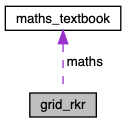
\includegraphics[width=166pt]{classgrid__rkr__coll__graph}
\end{center}
\end{figure}
\subsection*{Public Member Functions}
\begin{DoxyCompactItemize}
\item 
\hyperlink{classgrid__rkr_a8c3f61553704783780b89fb19aeb400c}{grid\+\_\+rkr} ()
\item 
\hyperlink{classgrid__rkr_adc3dbfbeb1dcc1ac948b58d26a83ffd1}{grid\+\_\+rkr} (int n\+\_\+r\+\_\+, double R\+\_\+, int n\+\_\+m\+\_\+, \hyperlink{classmaths__textbook}{maths\+\_\+textbook} \&maths\+\_\+)
\end{DoxyCompactItemize}
\subsection*{Public Attributes}
\begin{DoxyCompactItemize}
\item 
Array\+Xd \hyperlink{classgrid__rkr_a0c68f261e53153368d0edab4c9a8ef88}{r}
\item 
Array\+Xd \hyperlink{classgrid__rkr_aa09a97ce2aa9975fb4d2c1ee5da98b26}{kr}
\item 
int \hyperlink{classgrid__rkr_a332c5e88e5c3a08e67b11254173d9530}{n\+\_\+r}
\item 
double \hyperlink{classgrid__rkr_a2da8ae00c520a66c9cac2784a2149dcb}{R}
\item 
int \hyperlink{classgrid__rkr_ae580ce329d0cc89097775a6f4297b2ea}{n\+\_\+m}
\end{DoxyCompactItemize}
\subsection*{Private Attributes}
\begin{DoxyCompactItemize}
\item 
\hyperlink{classmaths__textbook}{maths\+\_\+textbook} \hyperlink{classgrid__rkr_acea8f6ec250de1407b452253edfc1eb0}{maths}
\end{DoxyCompactItemize}


\subsection{Detailed Description}
Originally created by Patrick Anderson. Modified by Samuel Senior on 10/03/2017. \char`\"{}grid\+\_\+rkr\char`\"{} is a non-\/uniform radial grid. The spectral counterpart of this grid is evaluated and accessible. 

\subsection{Constructor \& Destructor Documentation}
\mbox{\Hypertarget{classgrid__rkr_a8c3f61553704783780b89fb19aeb400c}\label{classgrid__rkr_a8c3f61553704783780b89fb19aeb400c}} 
\index{grid\+\_\+rkr@{grid\+\_\+rkr}!grid\+\_\+rkr@{grid\+\_\+rkr}}
\index{grid\+\_\+rkr@{grid\+\_\+rkr}!grid\+\_\+rkr@{grid\+\_\+rkr}}
\subsubsection{\texorpdfstring{grid\+\_\+rkr()}{grid\_rkr()}\hspace{0.1cm}{\footnotesize\ttfamily [1/2]}}
{\footnotesize\ttfamily grid\+\_\+rkr\+::grid\+\_\+rkr (\begin{DoxyParamCaption}{ }\end{DoxyParamCaption})}

Default constructor \mbox{\Hypertarget{classgrid__rkr_adc3dbfbeb1dcc1ac948b58d26a83ffd1}\label{classgrid__rkr_adc3dbfbeb1dcc1ac948b58d26a83ffd1}} 
\index{grid\+\_\+rkr@{grid\+\_\+rkr}!grid\+\_\+rkr@{grid\+\_\+rkr}}
\index{grid\+\_\+rkr@{grid\+\_\+rkr}!grid\+\_\+rkr@{grid\+\_\+rkr}}
\subsubsection{\texorpdfstring{grid\+\_\+rkr()}{grid\_rkr()}\hspace{0.1cm}{\footnotesize\ttfamily [2/2]}}
{\footnotesize\ttfamily grid\+\_\+rkr\+::grid\+\_\+rkr (\begin{DoxyParamCaption}\item[{int}]{n\+\_\+r\+\_\+,  }\item[{double}]{R\+\_\+,  }\item[{int}]{n\+\_\+m\+\_\+,  }\item[{\hyperlink{classmaths__textbook}{maths\+\_\+textbook} \&}]{maths\+\_\+ }\end{DoxyParamCaption})}

Parameterized constructor 

\subsection{Member Data Documentation}
\mbox{\Hypertarget{classgrid__rkr_aa09a97ce2aa9975fb4d2c1ee5da98b26}\label{classgrid__rkr_aa09a97ce2aa9975fb4d2c1ee5da98b26}} 
\index{grid\+\_\+rkr@{grid\+\_\+rkr}!kr@{kr}}
\index{kr@{kr}!grid\+\_\+rkr@{grid\+\_\+rkr}}
\subsubsection{\texorpdfstring{kr}{kr}}
{\footnotesize\ttfamily Array\+Xd grid\+\_\+rkr\+::kr}

\mbox{\Hypertarget{classgrid__rkr_acea8f6ec250de1407b452253edfc1eb0}\label{classgrid__rkr_acea8f6ec250de1407b452253edfc1eb0}} 
\index{grid\+\_\+rkr@{grid\+\_\+rkr}!maths@{maths}}
\index{maths@{maths}!grid\+\_\+rkr@{grid\+\_\+rkr}}
\subsubsection{\texorpdfstring{maths}{maths}}
{\footnotesize\ttfamily \hyperlink{classmaths__textbook}{maths\+\_\+textbook} grid\+\_\+rkr\+::maths\hspace{0.3cm}{\ttfamily [private]}}

\mbox{\Hypertarget{classgrid__rkr_ae580ce329d0cc89097775a6f4297b2ea}\label{classgrid__rkr_ae580ce329d0cc89097775a6f4297b2ea}} 
\index{grid\+\_\+rkr@{grid\+\_\+rkr}!n\+\_\+m@{n\+\_\+m}}
\index{n\+\_\+m@{n\+\_\+m}!grid\+\_\+rkr@{grid\+\_\+rkr}}
\subsubsection{\texorpdfstring{n\+\_\+m}{n\_m}}
{\footnotesize\ttfamily int grid\+\_\+rkr\+::n\+\_\+m}

\mbox{\Hypertarget{classgrid__rkr_a332c5e88e5c3a08e67b11254173d9530}\label{classgrid__rkr_a332c5e88e5c3a08e67b11254173d9530}} 
\index{grid\+\_\+rkr@{grid\+\_\+rkr}!n\+\_\+r@{n\+\_\+r}}
\index{n\+\_\+r@{n\+\_\+r}!grid\+\_\+rkr@{grid\+\_\+rkr}}
\subsubsection{\texorpdfstring{n\+\_\+r}{n\_r}}
{\footnotesize\ttfamily int grid\+\_\+rkr\+::n\+\_\+r}

\mbox{\Hypertarget{classgrid__rkr_a0c68f261e53153368d0edab4c9a8ef88}\label{classgrid__rkr_a0c68f261e53153368d0edab4c9a8ef88}} 
\index{grid\+\_\+rkr@{grid\+\_\+rkr}!r@{r}}
\index{r@{r}!grid\+\_\+rkr@{grid\+\_\+rkr}}
\subsubsection{\texorpdfstring{r}{r}}
{\footnotesize\ttfamily Array\+Xd grid\+\_\+rkr\+::r}

\mbox{\Hypertarget{classgrid__rkr_a2da8ae00c520a66c9cac2784a2149dcb}\label{classgrid__rkr_a2da8ae00c520a66c9cac2784a2149dcb}} 
\index{grid\+\_\+rkr@{grid\+\_\+rkr}!R@{R}}
\index{R@{R}!grid\+\_\+rkr@{grid\+\_\+rkr}}
\subsubsection{\texorpdfstring{R}{R}}
{\footnotesize\ttfamily double grid\+\_\+rkr\+::R}



The documentation for this class was generated from the following files\+:\begin{DoxyCompactItemize}
\item 
/home/sam/\+Project/\+X\+N\+L\+O/src/grid/\hyperlink{grid__rkr_8hpp}{grid\+\_\+rkr.\+hpp}\item 
/home/sam/\+Project/\+X\+N\+L\+O/src/grid/\hyperlink{grid__rkr_8cpp}{grid\+\_\+rkr.\+cpp}\end{DoxyCompactItemize}

\hypertarget{classgrid__tw}{}\section{grid\+\_\+tw Class Reference}
\label{classgrid__tw}\index{grid\+\_\+tw@{grid\+\_\+tw}}


{\ttfamily \#include $<$grid\+\_\+tw.\+hpp$>$}

\subsection*{Public Member Functions}
\begin{DoxyCompactItemize}
\item 
\hyperlink{classgrid__tw_af1e2316561c84a2262e374600895010d}{grid\+\_\+tw} ()
\item 
\hyperlink{classgrid__tw_a583d4c2b423305ef3806d6221ed3f543}{grid\+\_\+tw} (int N\+\_\+t\+\_\+, double T\+\_\+, double w\+\_\+active\+\_\+min\+\_\+, double w\+\_\+active\+\_\+max\+\_\+, \hyperlink{classmaths__textbook}{maths\+\_\+textbook} \&maths\+\_\+)
\end{DoxyCompactItemize}
\subsection*{Public Attributes}
\begin{DoxyCompactItemize}
\item 
Array\+Xd \hyperlink{classgrid__tw_a918f1e6d18056d0f6da08fe01089b9b0}{t}
\item 
Array\+Xd \hyperlink{classgrid__tw_a66922766c9dfe5c4667e55e678b134b9}{w\+\_\+active}
\item 
int \hyperlink{classgrid__tw_ac121ce740479f628bdaa54627540ad42}{n\+\_\+t}
\item 
int \hyperlink{classgrid__tw_a1fbf854a0f7bd025aa98671009602c5c}{n\+\_\+active}
\item 
int \hyperlink{classgrid__tw_a27d987fb3c8cbacf9cd152b83477f0d9}{w\+\_\+active\+\_\+min\+\_\+index}
\end{DoxyCompactItemize}


\subsection{Detailed Description}
Originally created by Patrick Anderson. Modified by Samuel Senior on 10/03/2017. \char`\"{}grid\+\_\+tw\char`\"{} is a linear temporal grid. The spectral counterpart of this grid is evaluated and made accessible. 

\subsection{Constructor \& Destructor Documentation}
\mbox{\Hypertarget{classgrid__tw_af1e2316561c84a2262e374600895010d}\label{classgrid__tw_af1e2316561c84a2262e374600895010d}} 
\index{grid\+\_\+tw@{grid\+\_\+tw}!grid\+\_\+tw@{grid\+\_\+tw}}
\index{grid\+\_\+tw@{grid\+\_\+tw}!grid\+\_\+tw@{grid\+\_\+tw}}
\subsubsection{\texorpdfstring{grid\+\_\+tw()}{grid\_tw()}\hspace{0.1cm}{\footnotesize\ttfamily [1/2]}}
{\footnotesize\ttfamily grid\+\_\+tw\+::grid\+\_\+tw (\begin{DoxyParamCaption}{ }\end{DoxyParamCaption})}

\mbox{\Hypertarget{classgrid__tw_a583d4c2b423305ef3806d6221ed3f543}\label{classgrid__tw_a583d4c2b423305ef3806d6221ed3f543}} 
\index{grid\+\_\+tw@{grid\+\_\+tw}!grid\+\_\+tw@{grid\+\_\+tw}}
\index{grid\+\_\+tw@{grid\+\_\+tw}!grid\+\_\+tw@{grid\+\_\+tw}}
\subsubsection{\texorpdfstring{grid\+\_\+tw()}{grid\_tw()}\hspace{0.1cm}{\footnotesize\ttfamily [2/2]}}
{\footnotesize\ttfamily grid\+\_\+tw\+::grid\+\_\+tw (\begin{DoxyParamCaption}\item[{int}]{n\+\_\+t\+\_\+,  }\item[{double}]{T\+\_\+,  }\item[{double}]{w\+\_\+active\+\_\+min\+\_\+,  }\item[{double}]{w\+\_\+active\+\_\+max\+\_\+,  }\item[{\hyperlink{classmaths__textbook}{maths\+\_\+textbook} \&}]{maths\+\_\+ }\end{DoxyParamCaption})}

Parameterized Constructor 

\subsection{Member Data Documentation}
\mbox{\Hypertarget{classgrid__tw_a1fbf854a0f7bd025aa98671009602c5c}\label{classgrid__tw_a1fbf854a0f7bd025aa98671009602c5c}} 
\index{grid\+\_\+tw@{grid\+\_\+tw}!n\+\_\+active@{n\+\_\+active}}
\index{n\+\_\+active@{n\+\_\+active}!grid\+\_\+tw@{grid\+\_\+tw}}
\subsubsection{\texorpdfstring{n\+\_\+active}{n\_active}}
{\footnotesize\ttfamily int grid\+\_\+tw\+::n\+\_\+active}

\mbox{\Hypertarget{classgrid__tw_ac121ce740479f628bdaa54627540ad42}\label{classgrid__tw_ac121ce740479f628bdaa54627540ad42}} 
\index{grid\+\_\+tw@{grid\+\_\+tw}!n\+\_\+t@{n\+\_\+t}}
\index{n\+\_\+t@{n\+\_\+t}!grid\+\_\+tw@{grid\+\_\+tw}}
\subsubsection{\texorpdfstring{n\+\_\+t}{n\_t}}
{\footnotesize\ttfamily int grid\+\_\+tw\+::n\+\_\+t}

\mbox{\Hypertarget{classgrid__tw_a918f1e6d18056d0f6da08fe01089b9b0}\label{classgrid__tw_a918f1e6d18056d0f6da08fe01089b9b0}} 
\index{grid\+\_\+tw@{grid\+\_\+tw}!t@{t}}
\index{t@{t}!grid\+\_\+tw@{grid\+\_\+tw}}
\subsubsection{\texorpdfstring{t}{t}}
{\footnotesize\ttfamily Array\+Xd grid\+\_\+tw\+::t}

\mbox{\Hypertarget{classgrid__tw_a66922766c9dfe5c4667e55e678b134b9}\label{classgrid__tw_a66922766c9dfe5c4667e55e678b134b9}} 
\index{grid\+\_\+tw@{grid\+\_\+tw}!w\+\_\+active@{w\+\_\+active}}
\index{w\+\_\+active@{w\+\_\+active}!grid\+\_\+tw@{grid\+\_\+tw}}
\subsubsection{\texorpdfstring{w\+\_\+active}{w\_active}}
{\footnotesize\ttfamily Array\+Xd grid\+\_\+tw\+::w\+\_\+active}

\mbox{\Hypertarget{classgrid__tw_a27d987fb3c8cbacf9cd152b83477f0d9}\label{classgrid__tw_a27d987fb3c8cbacf9cd152b83477f0d9}} 
\index{grid\+\_\+tw@{grid\+\_\+tw}!w\+\_\+active\+\_\+min\+\_\+index@{w\+\_\+active\+\_\+min\+\_\+index}}
\index{w\+\_\+active\+\_\+min\+\_\+index@{w\+\_\+active\+\_\+min\+\_\+index}!grid\+\_\+tw@{grid\+\_\+tw}}
\subsubsection{\texorpdfstring{w\+\_\+active\+\_\+min\+\_\+index}{w\_active\_min\_index}}
{\footnotesize\ttfamily int grid\+\_\+tw\+::w\+\_\+active\+\_\+min\+\_\+index}



The documentation for this class was generated from the following files\+:\begin{DoxyCompactItemize}
\item 
/home/sam/\+Project/\+X\+N\+L\+O/src/grid/\hyperlink{grid__tw_8hpp}{grid\+\_\+tw.\+hpp}\item 
/home/sam/\+Project/\+X\+N\+L\+O/src/grid/\hyperlink{grid__tw_8cpp}{grid\+\_\+tw.\+cpp}\end{DoxyCompactItemize}

\input{class_x_n_l_o_1_1grid__tw}
\input{classgrid__xkx}
\hypertarget{class_h_h__source}{}\section{H\+H\+\_\+source Class Reference}
\label{class_h_h__source}\index{H\+H\+\_\+source@{H\+H\+\_\+source}}


{\ttfamily \#include $<$H\+H\+\_\+source.\+hpp$>$}



Collaboration diagram for H\+H\+\_\+source\+:\nopagebreak
\begin{figure}[H]
\begin{center}
\leavevmode
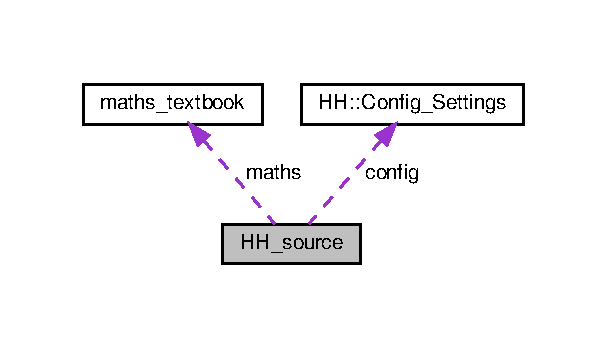
\includegraphics[width=292pt]{class_h_h__source__coll__graph}
\end{center}
\end{figure}
\subsection*{Public Member Functions}
\begin{DoxyCompactItemize}
\item 
\hyperlink{class_h_h__source_a0b3c052d274495b4f90fb09d15fff9fa}{H\+H\+\_\+source} ()
\item 
Array\+X\+Xcd \hyperlink{class_h_h__source_a059c934be1aaa0ed411fea5374bb2428}{Get\+Source} (int \hyperlink{class_h_h__source_a6631481cc1bea05ab564cb1841644a12}{file\+Number}, \hyperlink{class_h_h_1_1_config___settings}{H\+H\+::\+Config\+\_\+\+Settings} \hyperlink{class_h_h__source_adbab95c09c583e2aeebbb4679e6998e8}{config}, \hyperlink{classmaths__textbook}{maths\+\_\+textbook} \hyperlink{class_h_h__source_a93637ad30af846dd04eb741437114f8f}{maths})
\end{DoxyCompactItemize}
\subsection*{Private Attributes}
\begin{DoxyCompactItemize}
\item 
int \hyperlink{class_h_h__source_a6631481cc1bea05ab564cb1841644a12}{file\+Number}
\item 
\hyperlink{class_h_h_1_1_config___settings}{H\+H\+::\+Config\+\_\+\+Settings} \hyperlink{class_h_h__source_adbab95c09c583e2aeebbb4679e6998e8}{config}
\item 
\hyperlink{classmaths__textbook}{maths\+\_\+textbook} \hyperlink{class_h_h__source_a93637ad30af846dd04eb741437114f8f}{maths}
\end{DoxyCompactItemize}


\subsection{Constructor \& Destructor Documentation}
\mbox{\Hypertarget{class_h_h__source_a0b3c052d274495b4f90fb09d15fff9fa}\label{class_h_h__source_a0b3c052d274495b4f90fb09d15fff9fa}} 
\index{H\+H\+\_\+source@{H\+H\+\_\+source}!H\+H\+\_\+source@{H\+H\+\_\+source}}
\index{H\+H\+\_\+source@{H\+H\+\_\+source}!H\+H\+\_\+source@{H\+H\+\_\+source}}
\subsubsection{\texorpdfstring{H\+H\+\_\+source()}{HH\_source()}}
{\footnotesize\ttfamily H\+H\+\_\+source\+::\+H\+H\+\_\+source (\begin{DoxyParamCaption}{ }\end{DoxyParamCaption})}



\subsection{Member Function Documentation}
\mbox{\Hypertarget{class_h_h__source_a059c934be1aaa0ed411fea5374bb2428}\label{class_h_h__source_a059c934be1aaa0ed411fea5374bb2428}} 
\index{H\+H\+\_\+source@{H\+H\+\_\+source}!Get\+Source@{Get\+Source}}
\index{Get\+Source@{Get\+Source}!H\+H\+\_\+source@{H\+H\+\_\+source}}
\subsubsection{\texorpdfstring{Get\+Source()}{GetSource()}}
{\footnotesize\ttfamily Array\+X\+Xcd H\+H\+\_\+source\+::\+Get\+Source (\begin{DoxyParamCaption}\item[{int}]{file\+Number,  }\item[{\hyperlink{class_h_h_1_1_config___settings}{H\+H\+::\+Config\+\_\+\+Settings}}]{config,  }\item[{\hyperlink{classmaths__textbook}{maths\+\_\+textbook}}]{maths }\end{DoxyParamCaption})}



\subsection{Member Data Documentation}
\mbox{\Hypertarget{class_h_h__source_adbab95c09c583e2aeebbb4679e6998e8}\label{class_h_h__source_adbab95c09c583e2aeebbb4679e6998e8}} 
\index{H\+H\+\_\+source@{H\+H\+\_\+source}!config@{config}}
\index{config@{config}!H\+H\+\_\+source@{H\+H\+\_\+source}}
\subsubsection{\texorpdfstring{config}{config}}
{\footnotesize\ttfamily \hyperlink{class_h_h_1_1_config___settings}{H\+H\+::\+Config\+\_\+\+Settings} H\+H\+\_\+source\+::config\hspace{0.3cm}{\ttfamily [private]}}

\mbox{\Hypertarget{class_h_h__source_a6631481cc1bea05ab564cb1841644a12}\label{class_h_h__source_a6631481cc1bea05ab564cb1841644a12}} 
\index{H\+H\+\_\+source@{H\+H\+\_\+source}!file\+Number@{file\+Number}}
\index{file\+Number@{file\+Number}!H\+H\+\_\+source@{H\+H\+\_\+source}}
\subsubsection{\texorpdfstring{file\+Number}{fileNumber}}
{\footnotesize\ttfamily int H\+H\+\_\+source\+::file\+Number\hspace{0.3cm}{\ttfamily [private]}}

\mbox{\Hypertarget{class_h_h__source_a93637ad30af846dd04eb741437114f8f}\label{class_h_h__source_a93637ad30af846dd04eb741437114f8f}} 
\index{H\+H\+\_\+source@{H\+H\+\_\+source}!maths@{maths}}
\index{maths@{maths}!H\+H\+\_\+source@{H\+H\+\_\+source}}
\subsubsection{\texorpdfstring{maths}{maths}}
{\footnotesize\ttfamily \hyperlink{classmaths__textbook}{maths\+\_\+textbook} H\+H\+\_\+source\+::maths\hspace{0.3cm}{\ttfamily [private]}}



The documentation for this class was generated from the following files\+:\begin{DoxyCompactItemize}
\item 
/\+Users/sms1n16/\+Project/\+X\+N\+L\+O/src/\+H\+H\+G\+P/\hyperlink{_h_h__source_8hpp}{H\+H\+\_\+source.\+hpp}\item 
/\+Users/sms1n16/\+Project/\+X\+N\+L\+O/src/\+H\+H\+G\+P/\hyperlink{_h_h__source_8cpp}{H\+H\+\_\+source.\+cpp}\end{DoxyCompactItemize}

\input{class_h_h_g_p}
\hypertarget{class_i_o}{}\section{IO Class Reference}
\label{class_i_o}\index{IO@{IO}}


{\ttfamily \#include $<$I\+O.\+hpp$>$}

\subsection*{Public Member Functions}
\begin{DoxyCompactItemize}
\item 
\hyperlink{class_i_o_a49b27a2ee79bce0de4e3ef163cbebd30}{IO} ()
\item 
void \hyperlink{class_i_o_aed76c50d1122060292bfb10181edc990}{read\+\_\+header} (const std\+::string path, bool print=true)
\item 
Array$<$ unsigned short, Dynamic, Dynamic $>$ \hyperlink{class_i_o_a0ba1550dc3c2b6fd4675bc03408b8d95}{read\+\_\+uint16} (const char $\ast$path\+\_\+, int \hyperlink{class_i_o_ab8aa1490df2e2e758766030afdae3a40}{N\+\_\+row\+\_\+}, int \hyperlink{class_i_o_a64aae2d2be35348233f8ddac4d6791f2}{N\+\_\+col\+\_\+})
\item 
Array\+X\+Xi \hyperlink{class_i_o_a7b78b5f726c5299423e72b2b44bce0c9}{read\+\_\+int} (const char $\ast$path\+\_\+, int \hyperlink{class_i_o_ab8aa1490df2e2e758766030afdae3a40}{N\+\_\+row\+\_\+}, int \hyperlink{class_i_o_a64aae2d2be35348233f8ddac4d6791f2}{N\+\_\+col\+\_\+})
\item 
Array\+X\+Xd \hyperlink{class_i_o_aa2d53b758b98c564688d00ca5236744e}{read\+\_\+double} (const std\+::string path, int \hyperlink{class_i_o_ab8aa1490df2e2e758766030afdae3a40}{N\+\_\+row\+\_\+}, int \hyperlink{class_i_o_a64aae2d2be35348233f8ddac4d6791f2}{N\+\_\+col\+\_\+}, bool print=true)
\item 
Array\+X\+Xd \hyperlink{class_i_o_a34ed8843269915cb0b4eb8719da3535d}{read\+\_\+double} (const std\+::string path, bool skip\+\_\+header=true, bool print=true)
\item 
Array\+X\+Xd \hyperlink{class_i_o_a3ddd4b5d95a8a5cfffb56cfcf7c186e1}{read\+\_\+ascii\+\_\+double} (const std\+::string path, int \hyperlink{class_i_o_ab8aa1490df2e2e758766030afdae3a40}{N\+\_\+row\+\_\+}, int \hyperlink{class_i_o_a64aae2d2be35348233f8ddac4d6791f2}{N\+\_\+col\+\_\+}, bool header=true)
\item 
void \hyperlink{class_i_o_a9a648215dc5e33abe2c5a8916fff06d4}{write\+\_\+double} (const std\+::string path\+\_\+, Array\+X\+Xd input\+\_\+, int \hyperlink{class_i_o_ab8aa1490df2e2e758766030afdae3a40}{N\+\_\+row\+\_\+}, int \hyperlink{class_i_o_a64aae2d2be35348233f8ddac4d6791f2}{N\+\_\+col\+\_\+}, bool print=true)
\item 
void \hyperlink{class_i_o_a0db950886bb1e6d5571330f771974c4e}{write\+\_\+header} (const std\+::string path\+\_\+, int \hyperlink{class_i_o_ab8aa1490df2e2e758766030afdae3a40}{N\+\_\+row\+\_\+}, int \hyperlink{class_i_o_a64aae2d2be35348233f8ddac4d6791f2}{N\+\_\+col\+\_\+}, bool print=true)
\item 
void \hyperlink{class_i_o_a0fd7211866348cd3acc26d1ed17c100c}{overwrite} (const std\+::string path, bool print=true)
\item 
void \hyperlink{class_i_o_a20602422f0a6615b265c96fc02523e6f}{write\+\_\+ascii\+\_\+double} (Array\+Xd data, std\+::string path, bool print=true)
\item 
{\footnotesize template$<$typename T $>$ }\\void \hyperlink{class_i_o_ac84ca0cd185f0df4ea871710120577d6}{write} (T output, std\+::string path, bool print=true)
\end{DoxyCompactItemize}
\subsection*{Public Attributes}
\begin{DoxyCompactItemize}
\item 
std\+::string \hyperlink{class_i_o_a254c13a437051a09be72f77173017576}{binary\+\_\+format}
\item 
int \hyperlink{class_i_o_aaf91ba1d8be1503b44b2b1b1b666303b}{binary\+\_\+format\+\_\+version}
\item 
int \hyperlink{class_i_o_ad5c0c344b35565bb355c5d714121787b}{binary\+\_\+format\+\_\+subversion}
\item 
int \hyperlink{class_i_o_a2a1699a4cde1ce8631ae0309bc75d336}{binary\+\_\+format\+\_\+len}
\item 
int \hyperlink{class_i_o_a39a8a0474a288522d847f6be0fb2403f}{data\+\_\+size}
\item 
int \hyperlink{class_i_o_a3af3bf77eacd18c1c50cbf78b46c4228}{double\+\_\+size}
\item 
int \hyperlink{class_i_o_ab8aa1490df2e2e758766030afdae3a40}{N\+\_\+row\+\_\+}
\item 
int \hyperlink{class_i_o_a64aae2d2be35348233f8ddac4d6791f2}{N\+\_\+col\+\_\+}
\item 
int \hyperlink{class_i_o_aee540c40b18d5f9990bf8d7e12cb0827}{header\+\_\+size}
\end{DoxyCompactItemize}


\subsection{Detailed Description}
Originally created by Patrick Anderson. Modified by Samuel Senior on 10/03/2017. \char`\"{}\+I\+O\char`\"{} objects enable reading/writing of binary files to/from Eigen arrays. 

\subsection{Constructor \& Destructor Documentation}
\mbox{\Hypertarget{class_i_o_a49b27a2ee79bce0de4e3ef163cbebd30}\label{class_i_o_a49b27a2ee79bce0de4e3ef163cbebd30}} 
\index{IO@{IO}!IO@{IO}}
\index{IO@{IO}!IO@{IO}}
\subsubsection{\texorpdfstring{I\+O()}{IO()}}
{\footnotesize\ttfamily I\+O\+::\+IO (\begin{DoxyParamCaption}{ }\end{DoxyParamCaption})}

Constructor 

\subsection{Member Function Documentation}
\mbox{\Hypertarget{class_i_o_a0fd7211866348cd3acc26d1ed17c100c}\label{class_i_o_a0fd7211866348cd3acc26d1ed17c100c}} 
\index{IO@{IO}!overwrite@{overwrite}}
\index{overwrite@{overwrite}!IO@{IO}}
\subsubsection{\texorpdfstring{overwrite()}{overwrite()}}
{\footnotesize\ttfamily void I\+O\+::overwrite (\begin{DoxyParamCaption}\item[{const std\+::string}]{path,  }\item[{bool}]{print = {\ttfamily true} }\end{DoxyParamCaption})}

Overwrites given binary file.\mbox{\Hypertarget{class_i_o_a3ddd4b5d95a8a5cfffb56cfcf7c186e1}\label{class_i_o_a3ddd4b5d95a8a5cfffb56cfcf7c186e1}} 
\index{IO@{IO}!read\+\_\+ascii\+\_\+double@{read\+\_\+ascii\+\_\+double}}
\index{read\+\_\+ascii\+\_\+double@{read\+\_\+ascii\+\_\+double}!IO@{IO}}
\subsubsection{\texorpdfstring{read\+\_\+ascii\+\_\+double()}{read\_ascii\_double()}}
{\footnotesize\ttfamily Array\+X\+Xd I\+O\+::read\+\_\+ascii\+\_\+double (\begin{DoxyParamCaption}\item[{const std\+::string}]{path,  }\item[{int}]{N\+\_\+row\+\_\+,  }\item[{int}]{N\+\_\+col\+\_\+,  }\item[{bool}]{header = {\ttfamily true} }\end{DoxyParamCaption})}

Read double to Eigen array from ascii file\mbox{\Hypertarget{class_i_o_aa2d53b758b98c564688d00ca5236744e}\label{class_i_o_aa2d53b758b98c564688d00ca5236744e}} 
\index{IO@{IO}!read\+\_\+double@{read\+\_\+double}}
\index{read\+\_\+double@{read\+\_\+double}!IO@{IO}}
\subsubsection{\texorpdfstring{read\+\_\+double()}{read\_double()}\hspace{0.1cm}{\footnotesize\ttfamily [1/2]}}
{\footnotesize\ttfamily Array\+X\+Xd I\+O\+::read\+\_\+double (\begin{DoxyParamCaption}\item[{const std\+::string}]{path,  }\item[{int}]{N\+\_\+row\+\_\+,  }\item[{int}]{N\+\_\+col\+\_\+,  }\item[{bool}]{print = {\ttfamily true} }\end{DoxyParamCaption})}

Read a two-\/dimensional array of doubles into an to Eigen array from a binary file. The number of rows and columns of the array are given by N\+\_\+row\+\_\+ and N\+\_\+col\+\_\+, as passed in from the function arguments.\mbox{\Hypertarget{class_i_o_a34ed8843269915cb0b4eb8719da3535d}\label{class_i_o_a34ed8843269915cb0b4eb8719da3535d}} 
\index{IO@{IO}!read\+\_\+double@{read\+\_\+double}}
\index{read\+\_\+double@{read\+\_\+double}!IO@{IO}}
\subsubsection{\texorpdfstring{read\+\_\+double()}{read\_double()}\hspace{0.1cm}{\footnotesize\ttfamily [2/2]}}
{\footnotesize\ttfamily Array\+X\+Xd I\+O\+::read\+\_\+double (\begin{DoxyParamCaption}\item[{const std\+::string}]{path,  }\item[{bool}]{skip\+\_\+header = {\ttfamily true},  }\item[{bool}]{print = {\ttfamily true} }\end{DoxyParamCaption})}

Read a two-\/dimensional array of doubles into an to Eigen array from a binary file. The number of rows and columns of the array are taken as the class variables N\+\_\+row\+\_\+ and N\+\_\+col\+\_\+.\mbox{\Hypertarget{class_i_o_aed76c50d1122060292bfb10181edc990}\label{class_i_o_aed76c50d1122060292bfb10181edc990}} 
\index{IO@{IO}!read\+\_\+header@{read\+\_\+header}}
\index{read\+\_\+header@{read\+\_\+header}!IO@{IO}}
\subsubsection{\texorpdfstring{read\+\_\+header()}{read\_header()}}
{\footnotesize\ttfamily void I\+O\+::read\+\_\+header (\begin{DoxyParamCaption}\item[{const std\+::string}]{path,  }\item[{bool}]{print = {\ttfamily true} }\end{DoxyParamCaption})}

Read the X\+N\+LO/\+U\+P\+PE binary header of a given binary file.

The header takes the form\+: \tabulinesep=1mm
\begin{longtabu} spread 0pt [c]{*{4}{|X[-1]}|}
\hline
\rowcolor{\tableheadbgcolor}\PBS\centering \textbf{ Offset }&\PBS\centering \textbf{ Size (Bytes) }&\PBS\centering \textbf{ Type/\+Contents }&\textbf{ Description  }\\\cline{1-4}
\endfirsthead
\hline
\endfoot
\hline
\rowcolor{\tableheadbgcolor}\PBS\centering \textbf{ Offset }&\PBS\centering \textbf{ Size (Bytes) }&\PBS\centering \textbf{ Type/\+Contents }&\textbf{ Description  }\\\cline{1-4}
\endhead
\PBS\centering 0 &\PBS\centering 4 &\PBS\centering \textquotesingle{}X\+N\+LO\textquotesingle{}/\textquotesingle{}U\+P\+PE\textquotesingle{} &Binary format name \\\cline{1-4}
\PBS\centering 4 &\PBS\centering 4 &\PBS\centering int &Version number \\\cline{1-4}
\PBS\centering 8 &\PBS\centering 4 &\PBS\centering int &Subversion number \\\cline{1-4}
\PBS\centering 12 &\PBS\centering 4 &\PBS\centering int &Size of header \\\cline{1-4}
\PBS\centering 16 &\PBS\centering 4 &\PBS\centering int &N\+\_\+row \\\cline{1-4}
\PBS\centering 20 &\PBS\centering 4 &\PBS\centering int &N\+\_\+col \\\cline{1-4}
\PBS\centering 24 &\PBS\centering 4 &\PBS\centering int &Total size of data \\\cline{1-4}
\PBS\centering 28 &\PBS\centering 4 &\PBS\centering int &Size of each double in the data \\\cline{1-4}
\end{longtabu}
That is to say, the first four bytes of an X\+N\+LO or U\+P\+PE binary header are the either the four characters \textquotesingle{}X\+N\+LO\textquotesingle{} or \textquotesingle{}U\+P\+PE\textquotesingle{}, used to specify which file type it is. The next four bytes give an integer, which is the version number. The next four give the subversion number as integer, and so on.\mbox{\Hypertarget{class_i_o_a7b78b5f726c5299423e72b2b44bce0c9}\label{class_i_o_a7b78b5f726c5299423e72b2b44bce0c9}} 
\index{IO@{IO}!read\+\_\+int@{read\+\_\+int}}
\index{read\+\_\+int@{read\+\_\+int}!IO@{IO}}
\subsubsection{\texorpdfstring{read\+\_\+int()}{read\_int()}}
{\footnotesize\ttfamily Array\+X\+Xi I\+O\+::read\+\_\+int (\begin{DoxyParamCaption}\item[{const char $\ast$}]{path\+\_\+,  }\item[{int}]{N\+\_\+row\+\_\+,  }\item[{int}]{N\+\_\+col\+\_\+ }\end{DoxyParamCaption})}

int\mbox{\Hypertarget{class_i_o_a0ba1550dc3c2b6fd4675bc03408b8d95}\label{class_i_o_a0ba1550dc3c2b6fd4675bc03408b8d95}} 
\index{IO@{IO}!read\+\_\+uint16@{read\+\_\+uint16}}
\index{read\+\_\+uint16@{read\+\_\+uint16}!IO@{IO}}
\subsubsection{\texorpdfstring{read\+\_\+uint16()}{read\_uint16()}}
{\footnotesize\ttfamily Array$<$ unsigned short, Dynamic, Dynamic $>$ I\+O\+::read\+\_\+uint16 (\begin{DoxyParamCaption}\item[{const char $\ast$}]{path\+\_\+,  }\item[{int}]{N\+\_\+row\+\_\+,  }\item[{int}]{N\+\_\+col\+\_\+ }\end{DoxyParamCaption})}

Read from binary file to N\+\_\+col\+\_\+ by N\+\_\+row\+\_\+ Eigen array uint16\mbox{\Hypertarget{class_i_o_ac84ca0cd185f0df4ea871710120577d6}\label{class_i_o_ac84ca0cd185f0df4ea871710120577d6}} 
\index{IO@{IO}!write@{write}}
\index{write@{write}!IO@{IO}}
\subsubsection{\texorpdfstring{write()}{write()}}
{\footnotesize\ttfamily template$<$typename T $>$ \\
void I\+O\+::write (\begin{DoxyParamCaption}\item[{T}]{output,  }\item[{std\+::string}]{path,  }\item[{bool}]{print = {\ttfamily true} }\end{DoxyParamCaption})}

\mbox{\Hypertarget{class_i_o_a20602422f0a6615b265c96fc02523e6f}\label{class_i_o_a20602422f0a6615b265c96fc02523e6f}} 
\index{IO@{IO}!write\+\_\+ascii\+\_\+double@{write\+\_\+ascii\+\_\+double}}
\index{write\+\_\+ascii\+\_\+double@{write\+\_\+ascii\+\_\+double}!IO@{IO}}
\subsubsection{\texorpdfstring{write\+\_\+ascii\+\_\+double()}{write\_ascii\_double()}}
{\footnotesize\ttfamily void I\+O\+::write\+\_\+ascii\+\_\+double (\begin{DoxyParamCaption}\item[{Array\+Xd}]{data,  }\item[{std\+::string}]{path,  }\item[{bool}]{print = {\ttfamily true} }\end{DoxyParamCaption})}

\mbox{\Hypertarget{class_i_o_a9a648215dc5e33abe2c5a8916fff06d4}\label{class_i_o_a9a648215dc5e33abe2c5a8916fff06d4}} 
\index{IO@{IO}!write\+\_\+double@{write\+\_\+double}}
\index{write\+\_\+double@{write\+\_\+double}!IO@{IO}}
\subsubsection{\texorpdfstring{write\+\_\+double()}{write\_double()}}
{\footnotesize\ttfamily void I\+O\+::write\+\_\+double (\begin{DoxyParamCaption}\item[{const std\+::string}]{path\+\_\+,  }\item[{Array\+X\+Xd}]{input\+\_\+,  }\item[{int}]{N\+\_\+row\+\_\+,  }\item[{int}]{N\+\_\+col\+\_\+,  }\item[{bool}]{print = {\ttfamily true} }\end{DoxyParamCaption})}

Write to binary file from N\+\_\+col\+\_\+ by N\+\_\+row\+\_\+ Eigen array double\mbox{\Hypertarget{class_i_o_a0db950886bb1e6d5571330f771974c4e}\label{class_i_o_a0db950886bb1e6d5571330f771974c4e}} 
\index{IO@{IO}!write\+\_\+header@{write\+\_\+header}}
\index{write\+\_\+header@{write\+\_\+header}!IO@{IO}}
\subsubsection{\texorpdfstring{write\+\_\+header()}{write\_header()}}
{\footnotesize\ttfamily void I\+O\+::write\+\_\+header (\begin{DoxyParamCaption}\item[{const std\+::string}]{path\+\_\+,  }\item[{int}]{N\+\_\+row\+\_\+,  }\item[{int}]{N\+\_\+col\+\_\+,  }\item[{bool}]{print = {\ttfamily true} }\end{DoxyParamCaption})}

Write \hyperlink{class_h_h_g_p}{H\+H\+GP} binary header to given binary file. Header takes the form\+: Offset Size (Bytes) Type/\+Contents Description 0 4 \textquotesingle{}\hyperlink{class_h_h_g_p}{H\+H\+GP}\textquotesingle{} Binary format name 4 4 int Version Number 8 4 int Subversion number 12 4 int Size of header 16 4 int N\+\_\+row 20 4 int N\+\_\+col 24 4 int Total size of data 28 4 int Size of each double in the data

\subsection{Member Data Documentation}
\mbox{\Hypertarget{class_i_o_a254c13a437051a09be72f77173017576}\label{class_i_o_a254c13a437051a09be72f77173017576}} 
\index{IO@{IO}!binary\+\_\+format@{binary\+\_\+format}}
\index{binary\+\_\+format@{binary\+\_\+format}!IO@{IO}}
\subsubsection{\texorpdfstring{binary\+\_\+format}{binary\_format}}
{\footnotesize\ttfamily std\+::string I\+O\+::binary\+\_\+format}

The binary format name. \mbox{\Hypertarget{class_i_o_a2a1699a4cde1ce8631ae0309bc75d336}\label{class_i_o_a2a1699a4cde1ce8631ae0309bc75d336}} 
\index{IO@{IO}!binary\+\_\+format\+\_\+len@{binary\+\_\+format\+\_\+len}}
\index{binary\+\_\+format\+\_\+len@{binary\+\_\+format\+\_\+len}!IO@{IO}}
\subsubsection{\texorpdfstring{binary\+\_\+format\+\_\+len}{binary\_format\_len}}
{\footnotesize\ttfamily int I\+O\+::binary\+\_\+format\+\_\+len}

The length of the binary format name. \mbox{\Hypertarget{class_i_o_ad5c0c344b35565bb355c5d714121787b}\label{class_i_o_ad5c0c344b35565bb355c5d714121787b}} 
\index{IO@{IO}!binary\+\_\+format\+\_\+subversion@{binary\+\_\+format\+\_\+subversion}}
\index{binary\+\_\+format\+\_\+subversion@{binary\+\_\+format\+\_\+subversion}!IO@{IO}}
\subsubsection{\texorpdfstring{binary\+\_\+format\+\_\+subversion}{binary\_format\_subversion}}
{\footnotesize\ttfamily int I\+O\+::binary\+\_\+format\+\_\+subversion}

The binary format subversion number. \mbox{\Hypertarget{class_i_o_aaf91ba1d8be1503b44b2b1b1b666303b}\label{class_i_o_aaf91ba1d8be1503b44b2b1b1b666303b}} 
\index{IO@{IO}!binary\+\_\+format\+\_\+version@{binary\+\_\+format\+\_\+version}}
\index{binary\+\_\+format\+\_\+version@{binary\+\_\+format\+\_\+version}!IO@{IO}}
\subsubsection{\texorpdfstring{binary\+\_\+format\+\_\+version}{binary\_format\_version}}
{\footnotesize\ttfamily int I\+O\+::binary\+\_\+format\+\_\+version}

The binary format version number. \mbox{\Hypertarget{class_i_o_a39a8a0474a288522d847f6be0fb2403f}\label{class_i_o_a39a8a0474a288522d847f6be0fb2403f}} 
\index{IO@{IO}!data\+\_\+size@{data\+\_\+size}}
\index{data\+\_\+size@{data\+\_\+size}!IO@{IO}}
\subsubsection{\texorpdfstring{data\+\_\+size}{data\_size}}
{\footnotesize\ttfamily int I\+O\+::data\+\_\+size}

The total number of elements of the data in the two dimensional array. \mbox{\Hypertarget{class_i_o_a3af3bf77eacd18c1c50cbf78b46c4228}\label{class_i_o_a3af3bf77eacd18c1c50cbf78b46c4228}} 
\index{IO@{IO}!double\+\_\+size@{double\+\_\+size}}
\index{double\+\_\+size@{double\+\_\+size}!IO@{IO}}
\subsubsection{\texorpdfstring{double\+\_\+size}{double\_size}}
{\footnotesize\ttfamily int I\+O\+::double\+\_\+size}

The size of a double in bytes. \mbox{\Hypertarget{class_i_o_aee540c40b18d5f9990bf8d7e12cb0827}\label{class_i_o_aee540c40b18d5f9990bf8d7e12cb0827}} 
\index{IO@{IO}!header\+\_\+size@{header\+\_\+size}}
\index{header\+\_\+size@{header\+\_\+size}!IO@{IO}}
\subsubsection{\texorpdfstring{header\+\_\+size}{header\_size}}
{\footnotesize\ttfamily int I\+O\+::header\+\_\+size}

The size of the header in bytes. \mbox{\Hypertarget{class_i_o_a64aae2d2be35348233f8ddac4d6791f2}\label{class_i_o_a64aae2d2be35348233f8ddac4d6791f2}} 
\index{IO@{IO}!N\+\_\+col\+\_\+@{N\+\_\+col\+\_\+}}
\index{N\+\_\+col\+\_\+@{N\+\_\+col\+\_\+}!IO@{IO}}
\subsubsection{\texorpdfstring{N\+\_\+col\+\_\+}{N\_col\_}}
{\footnotesize\ttfamily int I\+O\+::\+N\+\_\+col\+\_\+}

The number of columns to the two dimensional Eigen array. \mbox{\Hypertarget{class_i_o_ab8aa1490df2e2e758766030afdae3a40}\label{class_i_o_ab8aa1490df2e2e758766030afdae3a40}} 
\index{IO@{IO}!N\+\_\+row\+\_\+@{N\+\_\+row\+\_\+}}
\index{N\+\_\+row\+\_\+@{N\+\_\+row\+\_\+}!IO@{IO}}
\subsubsection{\texorpdfstring{N\+\_\+row\+\_\+}{N\_row\_}}
{\footnotesize\ttfamily int I\+O\+::\+N\+\_\+row\+\_\+}

The number of rows to the two dimensional Eigen array. 

The documentation for this class was generated from the following files\+:\begin{DoxyCompactItemize}
\item 
/home/sam/\+Project/\+X\+N\+L\+O/src/\+I\+O/\hyperlink{_i_o_8hpp}{I\+O.\+hpp}\item 
/home/sam/\+Project/\+X\+N\+L\+O/src/\+I\+O/\hyperlink{_i_o_8cpp}{I\+O.\+cpp}\end{DoxyCompactItemize}

\hypertarget{classkeldysh__gas}{}\section{keldysh\+\_\+gas Class Reference}
\label{classkeldysh__gas}\index{keldysh\+\_\+gas@{keldysh\+\_\+gas}}


{\ttfamily \#include $<$keldysh\+\_\+gas.\+hpp$>$}



Collaboration diagram for keldysh\+\_\+gas\+:\nopagebreak
\begin{figure}[H]
\begin{center}
\leavevmode
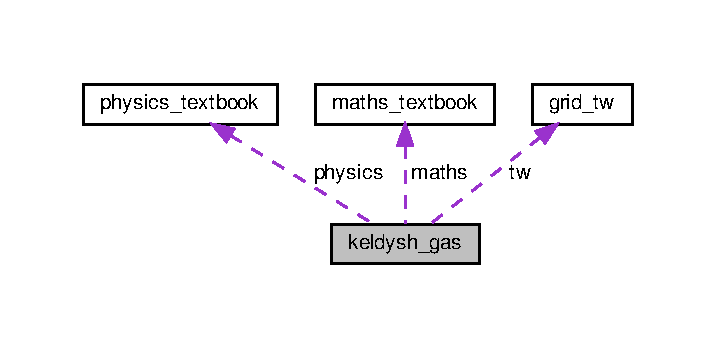
\includegraphics[width=344pt]{classkeldysh__gas__coll__graph}
\end{center}
\end{figure}
\subsection*{Public Member Functions}
\begin{DoxyCompactItemize}
\item 
\hyperlink{classkeldysh__gas_a25e559700c04e93efb560db511adbe72}{keldysh\+\_\+gas} ()
\item 
\hyperlink{classkeldysh__gas_a7889120c043b13492fa58878c5459099}{keldysh\+\_\+gas} (double press\+\_\+, std\+::string gas\+\_\+pressure\+\_\+profile\+\_\+)
\item 
\hyperlink{classkeldysh__gas_ae5510e8e448e96280f71b410907debf6}{keldysh\+\_\+gas} (double press\+\_\+, \hyperlink{classgrid__tw}{grid\+\_\+tw} \&tw\+\_\+, D\+F\+T\+I\+\_\+\+D\+E\+S\+C\+R\+I\+P\+T\+O\+R\+\_\+\+H\+A\+N\+D\+LE \&ft\+\_\+, \hyperlink{classmaths__textbook}{maths\+\_\+textbook} \&maths\+\_\+, std\+::string gas\+\_\+pressure\+\_\+profile\+\_\+)
\item 
double \hyperlink{classkeldysh__gas_acfa0604a6f00bce28b72b9a07fb79314}{atom\+\_\+density} (double z)
\item 
Array\+Xcd \hyperlink{classkeldysh__gas_a1cd65d1983cb6c5ff9d04eeb29e94dd5}{nl\+\_\+polarization} (Array\+Xd E\+\_\+t\+\_\+)
\item 
Array\+Xd \hyperlink{classkeldysh__gas_a42dc79816adcae9c25499baa7256ec10}{ionization\+\_\+rate} (Array\+Xd E\+\_\+t\+\_\+)
\item 
Array\+Xd \hyperlink{classkeldysh__gas_a8dddacdfabea4d6c3049088cc868715a}{electron\+\_\+density} (Array\+Xd W\+\_\+t\+\_\+, double z)
\item 
Array\+Xcd \hyperlink{classkeldysh__gas_a7d5f16951d622544d814518a37768411}{current\+\_\+density} (Array\+Xd E\+\_\+t\+\_\+, double z)
\end{DoxyCompactItemize}
\subsection*{Public Attributes}
\begin{DoxyCompactItemize}
\item 
double \hyperlink{classkeldysh__gas_a287e2c7a3081d8b65ba126288a3174bd}{atom\+\_\+density\+\_\+max}
\item 
double \hyperlink{classkeldysh__gas_a117691dd8b6fd06b34a73392c0e73e32}{z\+\_\+max}
\item 
double \hyperlink{classkeldysh__gas_ab0dee35b9ad45af3fca4a2079389e632}{inlet\+\_\+1}
\item 
double \hyperlink{classkeldysh__gas_a685d93a796afba55c6fcd6d61c7e2bf8}{inlet\+\_\+2}
\item 
double \hyperlink{classkeldysh__gas_a88f63ff18217c60729a67b10ee838ee4}{transition\+Length}
\item 
double \hyperlink{classkeldysh__gas_a752b70afe289a798cc0ab7b688b9ed3d}{U}
\item 
double \hyperlink{classkeldysh__gas_a7a66e438ff78b240fe419c0a426b1648}{C\+\_\+kl}
\item 
double \hyperlink{classkeldysh__gas_a22ba35c494b37c8a8e78db09d6d8748c}{n\+\_\+star}
\item 
double \hyperlink{classkeldysh__gas_a836c6a6c2f1bec80ea15344822a07ea5}{kappa}
\end{DoxyCompactItemize}
\subsection*{Private Types}
\begin{DoxyCompactItemize}
\item 
typedef double(keldysh\+\_\+gas\+::$\ast$ \hyperlink{classkeldysh__gas_ab47ad59b466eee349a7500555869b988}{atom\+\_\+density\+\_\+func\+\_\+ptr}) (double)
\end{DoxyCompactItemize}
\subsection*{Private Member Functions}
\begin{DoxyCompactItemize}
\item 
void \hyperlink{classkeldysh__gas_a051c59204ad55298d5632ac2eb4dd626}{set\+\_\+atom\+\_\+density\+\_\+ptr} (\hyperlink{classkeldysh__gas_ab47ad59b466eee349a7500555869b988}{atom\+\_\+density\+\_\+func\+\_\+ptr} ptr)
\item 
double \hyperlink{classkeldysh__gas_a9eac2e3d9a39a2358e9b6eb7f4a868c6}{capillary\+\_\+pressure\+\_\+profile} (double)
\item 
double \hyperlink{classkeldysh__gas_ad70cb5ac156d96492a164774b80e7cdc}{constant\+\_\+pressure\+\_\+profile} (double)
\end{DoxyCompactItemize}
\subsection*{Private Attributes}
\begin{DoxyCompactItemize}
\item 
\hyperlink{classphysics__textbook}{physics\+\_\+textbook} \hyperlink{classkeldysh__gas_a3b26e27ccf042ae2f89aa23e4252acf4}{physics}
\item 
\hyperlink{classmaths__textbook}{maths\+\_\+textbook} \hyperlink{classkeldysh__gas_a501614b541b9056bb05b378a39962524}{maths}
\item 
\hyperlink{classgrid__tw}{grid\+\_\+tw} \hyperlink{classkeldysh__gas_a1cd7129f9ba9d62f4084049e529cab49}{tw}
\item 
D\+F\+T\+I\+\_\+\+D\+E\+S\+C\+R\+I\+P\+T\+O\+R\+\_\+\+H\+A\+N\+D\+LE \hyperlink{classkeldysh__gas_ac635d55dcbdfcde7c34d77de5cd75af6}{ft}
\item 
std\+::string \hyperlink{classkeldysh__gas_a8e25aa7daf8df877e12db565294c3c72}{gas\+\_\+pressure\+\_\+profile}
\item 
\hyperlink{classkeldysh__gas_ab47ad59b466eee349a7500555869b988}{atom\+\_\+density\+\_\+func\+\_\+ptr} \hyperlink{classkeldysh__gas_aeb540c2cc32a862ab074638d53f172f7}{atom\+\_\+density\+\_\+func}
\end{DoxyCompactItemize}


\subsection{Detailed Description}
Originally created by Patrick Anderson. Modified by Samuel Senior on 10/03/2017. \char`\"{}keldysh\+\_\+gas\char`\"{} contains the medium response model. 

\subsection{Member Typedef Documentation}
\mbox{\Hypertarget{classkeldysh__gas_ab47ad59b466eee349a7500555869b988}\label{classkeldysh__gas_ab47ad59b466eee349a7500555869b988}} 
\index{keldysh\+\_\+gas@{keldysh\+\_\+gas}!atom\+\_\+density\+\_\+func\+\_\+ptr@{atom\+\_\+density\+\_\+func\+\_\+ptr}}
\index{atom\+\_\+density\+\_\+func\+\_\+ptr@{atom\+\_\+density\+\_\+func\+\_\+ptr}!keldysh\+\_\+gas@{keldysh\+\_\+gas}}
\subsubsection{\texorpdfstring{atom\+\_\+density\+\_\+func\+\_\+ptr}{atom\_density\_func\_ptr}}
{\footnotesize\ttfamily typedef double(keldysh\+\_\+gas\+::$\ast$ keldysh\+\_\+gas\+::atom\+\_\+density\+\_\+func\+\_\+ptr) (double)\hspace{0.3cm}{\ttfamily [private]}}



\subsection{Constructor \& Destructor Documentation}
\mbox{\Hypertarget{classkeldysh__gas_a25e559700c04e93efb560db511adbe72}\label{classkeldysh__gas_a25e559700c04e93efb560db511adbe72}} 
\index{keldysh\+\_\+gas@{keldysh\+\_\+gas}!keldysh\+\_\+gas@{keldysh\+\_\+gas}}
\index{keldysh\+\_\+gas@{keldysh\+\_\+gas}!keldysh\+\_\+gas@{keldysh\+\_\+gas}}
\subsubsection{\texorpdfstring{keldysh\+\_\+gas()}{keldysh\_gas()}\hspace{0.1cm}{\footnotesize\ttfamily [1/3]}}
{\footnotesize\ttfamily keldysh\+\_\+gas\+::keldysh\+\_\+gas (\begin{DoxyParamCaption}{ }\end{DoxyParamCaption})}

Constructor \mbox{\Hypertarget{classkeldysh__gas_a7889120c043b13492fa58878c5459099}\label{classkeldysh__gas_a7889120c043b13492fa58878c5459099}} 
\index{keldysh\+\_\+gas@{keldysh\+\_\+gas}!keldysh\+\_\+gas@{keldysh\+\_\+gas}}
\index{keldysh\+\_\+gas@{keldysh\+\_\+gas}!keldysh\+\_\+gas@{keldysh\+\_\+gas}}
\subsubsection{\texorpdfstring{keldysh\+\_\+gas()}{keldysh\_gas()}\hspace{0.1cm}{\footnotesize\ttfamily [2/3]}}
{\footnotesize\ttfamily keldysh\+\_\+gas\+::keldysh\+\_\+gas (\begin{DoxyParamCaption}\item[{double}]{press\+\_\+,  }\item[{std\+::string}]{gas\+\_\+pressure\+\_\+profile\+\_\+ }\end{DoxyParamCaption})}

\mbox{\Hypertarget{classkeldysh__gas_ae5510e8e448e96280f71b410907debf6}\label{classkeldysh__gas_ae5510e8e448e96280f71b410907debf6}} 
\index{keldysh\+\_\+gas@{keldysh\+\_\+gas}!keldysh\+\_\+gas@{keldysh\+\_\+gas}}
\index{keldysh\+\_\+gas@{keldysh\+\_\+gas}!keldysh\+\_\+gas@{keldysh\+\_\+gas}}
\subsubsection{\texorpdfstring{keldysh\+\_\+gas()}{keldysh\_gas()}\hspace{0.1cm}{\footnotesize\ttfamily [3/3]}}
{\footnotesize\ttfamily keldysh\+\_\+gas\+::keldysh\+\_\+gas (\begin{DoxyParamCaption}\item[{double}]{press\+\_\+,  }\item[{\hyperlink{classgrid__tw}{grid\+\_\+tw} \&}]{tw\+\_\+,  }\item[{D\+F\+T\+I\+\_\+\+D\+E\+S\+C\+R\+I\+P\+T\+O\+R\+\_\+\+H\+A\+N\+D\+LE \&}]{ft\+\_\+,  }\item[{\hyperlink{classmaths__textbook}{maths\+\_\+textbook} \&}]{maths\+\_\+,  }\item[{std\+::string}]{gas\+\_\+pressure\+\_\+profile\+\_\+ }\end{DoxyParamCaption})}



\subsection{Member Function Documentation}
\mbox{\Hypertarget{classkeldysh__gas_acfa0604a6f00bce28b72b9a07fb79314}\label{classkeldysh__gas_acfa0604a6f00bce28b72b9a07fb79314}} 
\index{keldysh\+\_\+gas@{keldysh\+\_\+gas}!atom\+\_\+density@{atom\+\_\+density}}
\index{atom\+\_\+density@{atom\+\_\+density}!keldysh\+\_\+gas@{keldysh\+\_\+gas}}
\subsubsection{\texorpdfstring{atom\+\_\+density()}{atom\_density()}}
{\footnotesize\ttfamily double keldysh\+\_\+gas\+::atom\+\_\+density (\begin{DoxyParamCaption}\item[{double}]{z }\end{DoxyParamCaption})}

\mbox{\Hypertarget{classkeldysh__gas_a9eac2e3d9a39a2358e9b6eb7f4a868c6}\label{classkeldysh__gas_a9eac2e3d9a39a2358e9b6eb7f4a868c6}} 
\index{keldysh\+\_\+gas@{keldysh\+\_\+gas}!capillary\+\_\+pressure\+\_\+profile@{capillary\+\_\+pressure\+\_\+profile}}
\index{capillary\+\_\+pressure\+\_\+profile@{capillary\+\_\+pressure\+\_\+profile}!keldysh\+\_\+gas@{keldysh\+\_\+gas}}
\subsubsection{\texorpdfstring{capillary\+\_\+pressure\+\_\+profile()}{capillary\_pressure\_profile()}}
{\footnotesize\ttfamily double keldysh\+\_\+gas\+::capillary\+\_\+pressure\+\_\+profile (\begin{DoxyParamCaption}\item[{double}]{z }\end{DoxyParamCaption})\hspace{0.3cm}{\ttfamily [private]}}

\mbox{\Hypertarget{classkeldysh__gas_ad70cb5ac156d96492a164774b80e7cdc}\label{classkeldysh__gas_ad70cb5ac156d96492a164774b80e7cdc}} 
\index{keldysh\+\_\+gas@{keldysh\+\_\+gas}!constant\+\_\+pressure\+\_\+profile@{constant\+\_\+pressure\+\_\+profile}}
\index{constant\+\_\+pressure\+\_\+profile@{constant\+\_\+pressure\+\_\+profile}!keldysh\+\_\+gas@{keldysh\+\_\+gas}}
\subsubsection{\texorpdfstring{constant\+\_\+pressure\+\_\+profile()}{constant\_pressure\_profile()}}
{\footnotesize\ttfamily double keldysh\+\_\+gas\+::constant\+\_\+pressure\+\_\+profile (\begin{DoxyParamCaption}\item[{double}]{z }\end{DoxyParamCaption})\hspace{0.3cm}{\ttfamily [private]}}

\mbox{\Hypertarget{classkeldysh__gas_a7d5f16951d622544d814518a37768411}\label{classkeldysh__gas_a7d5f16951d622544d814518a37768411}} 
\index{keldysh\+\_\+gas@{keldysh\+\_\+gas}!current\+\_\+density@{current\+\_\+density}}
\index{current\+\_\+density@{current\+\_\+density}!keldysh\+\_\+gas@{keldysh\+\_\+gas}}
\subsubsection{\texorpdfstring{current\+\_\+density()}{current\_density()}}
{\footnotesize\ttfamily Array\+Xcd keldysh\+\_\+gas\+::current\+\_\+density (\begin{DoxyParamCaption}\item[{Array\+Xd}]{E\+\_\+t\+\_\+,  }\item[{double}]{z }\end{DoxyParamCaption})}

Evaluate Current density for active frequencies \mbox{\Hypertarget{classkeldysh__gas_a8dddacdfabea4d6c3049088cc868715a}\label{classkeldysh__gas_a8dddacdfabea4d6c3049088cc868715a}} 
\index{keldysh\+\_\+gas@{keldysh\+\_\+gas}!electron\+\_\+density@{electron\+\_\+density}}
\index{electron\+\_\+density@{electron\+\_\+density}!keldysh\+\_\+gas@{keldysh\+\_\+gas}}
\subsubsection{\texorpdfstring{electron\+\_\+density()}{electron\_density()}}
{\footnotesize\ttfamily Array\+Xd keldysh\+\_\+gas\+::electron\+\_\+density (\begin{DoxyParamCaption}\item[{Array\+Xd}]{W\+\_\+t\+\_\+,  }\item[{double}]{z }\end{DoxyParamCaption})}

Calculate free electron density (solve rate equations) \mbox{\Hypertarget{classkeldysh__gas_a42dc79816adcae9c25499baa7256ec10}\label{classkeldysh__gas_a42dc79816adcae9c25499baa7256ec10}} 
\index{keldysh\+\_\+gas@{keldysh\+\_\+gas}!ionization\+\_\+rate@{ionization\+\_\+rate}}
\index{ionization\+\_\+rate@{ionization\+\_\+rate}!keldysh\+\_\+gas@{keldysh\+\_\+gas}}
\subsubsection{\texorpdfstring{ionization\+\_\+rate()}{ionization\_rate()}}
{\footnotesize\ttfamily Array\+Xd keldysh\+\_\+gas\+::ionization\+\_\+rate (\begin{DoxyParamCaption}\item[{Array\+Xd}]{E\+\_\+t\+\_\+ }\end{DoxyParamCaption})}

Calulate ionization rate (Popov, 2004) \mbox{\Hypertarget{classkeldysh__gas_a1cd65d1983cb6c5ff9d04eeb29e94dd5}\label{classkeldysh__gas_a1cd65d1983cb6c5ff9d04eeb29e94dd5}} 
\index{keldysh\+\_\+gas@{keldysh\+\_\+gas}!nl\+\_\+polarization@{nl\+\_\+polarization}}
\index{nl\+\_\+polarization@{nl\+\_\+polarization}!keldysh\+\_\+gas@{keldysh\+\_\+gas}}
\subsubsection{\texorpdfstring{nl\+\_\+polarization()}{nl\_polarization()}}
{\footnotesize\ttfamily Array\+Xcd keldysh\+\_\+gas\+::nl\+\_\+polarization (\begin{DoxyParamCaption}\item[{Array\+Xd}]{E\+\_\+t\+\_\+ }\end{DoxyParamCaption})}

Evaluate nonlinear polarization for active frequencies \mbox{\Hypertarget{classkeldysh__gas_a051c59204ad55298d5632ac2eb4dd626}\label{classkeldysh__gas_a051c59204ad55298d5632ac2eb4dd626}} 
\index{keldysh\+\_\+gas@{keldysh\+\_\+gas}!set\+\_\+atom\+\_\+density\+\_\+ptr@{set\+\_\+atom\+\_\+density\+\_\+ptr}}
\index{set\+\_\+atom\+\_\+density\+\_\+ptr@{set\+\_\+atom\+\_\+density\+\_\+ptr}!keldysh\+\_\+gas@{keldysh\+\_\+gas}}
\subsubsection{\texorpdfstring{set\+\_\+atom\+\_\+density\+\_\+ptr()}{set\_atom\_density\_ptr()}}
{\footnotesize\ttfamily void keldysh\+\_\+gas\+::set\+\_\+atom\+\_\+density\+\_\+ptr (\begin{DoxyParamCaption}\item[{\hyperlink{classkeldysh__gas_ab47ad59b466eee349a7500555869b988}{atom\+\_\+density\+\_\+func\+\_\+ptr}}]{ptr }\end{DoxyParamCaption})\hspace{0.3cm}{\ttfamily [private]}}



\subsection{Member Data Documentation}
\mbox{\Hypertarget{classkeldysh__gas_aeb540c2cc32a862ab074638d53f172f7}\label{classkeldysh__gas_aeb540c2cc32a862ab074638d53f172f7}} 
\index{keldysh\+\_\+gas@{keldysh\+\_\+gas}!atom\+\_\+density\+\_\+func@{atom\+\_\+density\+\_\+func}}
\index{atom\+\_\+density\+\_\+func@{atom\+\_\+density\+\_\+func}!keldysh\+\_\+gas@{keldysh\+\_\+gas}}
\subsubsection{\texorpdfstring{atom\+\_\+density\+\_\+func}{atom\_density\_func}}
{\footnotesize\ttfamily \hyperlink{classkeldysh__gas_ab47ad59b466eee349a7500555869b988}{atom\+\_\+density\+\_\+func\+\_\+ptr} keldysh\+\_\+gas\+::atom\+\_\+density\+\_\+func\hspace{0.3cm}{\ttfamily [private]}}

\mbox{\Hypertarget{classkeldysh__gas_a287e2c7a3081d8b65ba126288a3174bd}\label{classkeldysh__gas_a287e2c7a3081d8b65ba126288a3174bd}} 
\index{keldysh\+\_\+gas@{keldysh\+\_\+gas}!atom\+\_\+density\+\_\+max@{atom\+\_\+density\+\_\+max}}
\index{atom\+\_\+density\+\_\+max@{atom\+\_\+density\+\_\+max}!keldysh\+\_\+gas@{keldysh\+\_\+gas}}
\subsubsection{\texorpdfstring{atom\+\_\+density\+\_\+max}{atom\_density\_max}}
{\footnotesize\ttfamily double keldysh\+\_\+gas\+::atom\+\_\+density\+\_\+max}

\mbox{\Hypertarget{classkeldysh__gas_a7a66e438ff78b240fe419c0a426b1648}\label{classkeldysh__gas_a7a66e438ff78b240fe419c0a426b1648}} 
\index{keldysh\+\_\+gas@{keldysh\+\_\+gas}!C\+\_\+kl@{C\+\_\+kl}}
\index{C\+\_\+kl@{C\+\_\+kl}!keldysh\+\_\+gas@{keldysh\+\_\+gas}}
\subsubsection{\texorpdfstring{C\+\_\+kl}{C\_kl}}
{\footnotesize\ttfamily double keldysh\+\_\+gas\+::\+C\+\_\+kl}

\mbox{\Hypertarget{classkeldysh__gas_ac635d55dcbdfcde7c34d77de5cd75af6}\label{classkeldysh__gas_ac635d55dcbdfcde7c34d77de5cd75af6}} 
\index{keldysh\+\_\+gas@{keldysh\+\_\+gas}!ft@{ft}}
\index{ft@{ft}!keldysh\+\_\+gas@{keldysh\+\_\+gas}}
\subsubsection{\texorpdfstring{ft}{ft}}
{\footnotesize\ttfamily D\+F\+T\+I\+\_\+\+D\+E\+S\+C\+R\+I\+P\+T\+O\+R\+\_\+\+H\+A\+N\+D\+LE keldysh\+\_\+gas\+::ft\hspace{0.3cm}{\ttfamily [private]}}

\mbox{\Hypertarget{classkeldysh__gas_a8e25aa7daf8df877e12db565294c3c72}\label{classkeldysh__gas_a8e25aa7daf8df877e12db565294c3c72}} 
\index{keldysh\+\_\+gas@{keldysh\+\_\+gas}!gas\+\_\+pressure\+\_\+profile@{gas\+\_\+pressure\+\_\+profile}}
\index{gas\+\_\+pressure\+\_\+profile@{gas\+\_\+pressure\+\_\+profile}!keldysh\+\_\+gas@{keldysh\+\_\+gas}}
\subsubsection{\texorpdfstring{gas\+\_\+pressure\+\_\+profile}{gas\_pressure\_profile}}
{\footnotesize\ttfamily std\+::string keldysh\+\_\+gas\+::gas\+\_\+pressure\+\_\+profile\hspace{0.3cm}{\ttfamily [private]}}

\mbox{\Hypertarget{classkeldysh__gas_ab0dee35b9ad45af3fca4a2079389e632}\label{classkeldysh__gas_ab0dee35b9ad45af3fca4a2079389e632}} 
\index{keldysh\+\_\+gas@{keldysh\+\_\+gas}!inlet\+\_\+1@{inlet\+\_\+1}}
\index{inlet\+\_\+1@{inlet\+\_\+1}!keldysh\+\_\+gas@{keldysh\+\_\+gas}}
\subsubsection{\texorpdfstring{inlet\+\_\+1}{inlet\_1}}
{\footnotesize\ttfamily double keldysh\+\_\+gas\+::inlet\+\_\+1}

\mbox{\Hypertarget{classkeldysh__gas_a685d93a796afba55c6fcd6d61c7e2bf8}\label{classkeldysh__gas_a685d93a796afba55c6fcd6d61c7e2bf8}} 
\index{keldysh\+\_\+gas@{keldysh\+\_\+gas}!inlet\+\_\+2@{inlet\+\_\+2}}
\index{inlet\+\_\+2@{inlet\+\_\+2}!keldysh\+\_\+gas@{keldysh\+\_\+gas}}
\subsubsection{\texorpdfstring{inlet\+\_\+2}{inlet\_2}}
{\footnotesize\ttfamily double keldysh\+\_\+gas\+::inlet\+\_\+2}

\mbox{\Hypertarget{classkeldysh__gas_a836c6a6c2f1bec80ea15344822a07ea5}\label{classkeldysh__gas_a836c6a6c2f1bec80ea15344822a07ea5}} 
\index{keldysh\+\_\+gas@{keldysh\+\_\+gas}!kappa@{kappa}}
\index{kappa@{kappa}!keldysh\+\_\+gas@{keldysh\+\_\+gas}}
\subsubsection{\texorpdfstring{kappa}{kappa}}
{\footnotesize\ttfamily double keldysh\+\_\+gas\+::kappa}

\mbox{\Hypertarget{classkeldysh__gas_a501614b541b9056bb05b378a39962524}\label{classkeldysh__gas_a501614b541b9056bb05b378a39962524}} 
\index{keldysh\+\_\+gas@{keldysh\+\_\+gas}!maths@{maths}}
\index{maths@{maths}!keldysh\+\_\+gas@{keldysh\+\_\+gas}}
\subsubsection{\texorpdfstring{maths}{maths}}
{\footnotesize\ttfamily \hyperlink{classmaths__textbook}{maths\+\_\+textbook} keldysh\+\_\+gas\+::maths\hspace{0.3cm}{\ttfamily [private]}}

\mbox{\Hypertarget{classkeldysh__gas_a22ba35c494b37c8a8e78db09d6d8748c}\label{classkeldysh__gas_a22ba35c494b37c8a8e78db09d6d8748c}} 
\index{keldysh\+\_\+gas@{keldysh\+\_\+gas}!n\+\_\+star@{n\+\_\+star}}
\index{n\+\_\+star@{n\+\_\+star}!keldysh\+\_\+gas@{keldysh\+\_\+gas}}
\subsubsection{\texorpdfstring{n\+\_\+star}{n\_star}}
{\footnotesize\ttfamily double keldysh\+\_\+gas\+::n\+\_\+star}

\mbox{\Hypertarget{classkeldysh__gas_a3b26e27ccf042ae2f89aa23e4252acf4}\label{classkeldysh__gas_a3b26e27ccf042ae2f89aa23e4252acf4}} 
\index{keldysh\+\_\+gas@{keldysh\+\_\+gas}!physics@{physics}}
\index{physics@{physics}!keldysh\+\_\+gas@{keldysh\+\_\+gas}}
\subsubsection{\texorpdfstring{physics}{physics}}
{\footnotesize\ttfamily \hyperlink{classphysics__textbook}{physics\+\_\+textbook} keldysh\+\_\+gas\+::physics\hspace{0.3cm}{\ttfamily [private]}}

\mbox{\Hypertarget{classkeldysh__gas_a88f63ff18217c60729a67b10ee838ee4}\label{classkeldysh__gas_a88f63ff18217c60729a67b10ee838ee4}} 
\index{keldysh\+\_\+gas@{keldysh\+\_\+gas}!transition\+Length@{transition\+Length}}
\index{transition\+Length@{transition\+Length}!keldysh\+\_\+gas@{keldysh\+\_\+gas}}
\subsubsection{\texorpdfstring{transition\+Length}{transitionLength}}
{\footnotesize\ttfamily double keldysh\+\_\+gas\+::transition\+Length}

\mbox{\Hypertarget{classkeldysh__gas_a1cd7129f9ba9d62f4084049e529cab49}\label{classkeldysh__gas_a1cd7129f9ba9d62f4084049e529cab49}} 
\index{keldysh\+\_\+gas@{keldysh\+\_\+gas}!tw@{tw}}
\index{tw@{tw}!keldysh\+\_\+gas@{keldysh\+\_\+gas}}
\subsubsection{\texorpdfstring{tw}{tw}}
{\footnotesize\ttfamily \hyperlink{classgrid__tw}{grid\+\_\+tw} keldysh\+\_\+gas\+::tw\hspace{0.3cm}{\ttfamily [private]}}

\mbox{\Hypertarget{classkeldysh__gas_a752b70afe289a798cc0ab7b688b9ed3d}\label{classkeldysh__gas_a752b70afe289a798cc0ab7b688b9ed3d}} 
\index{keldysh\+\_\+gas@{keldysh\+\_\+gas}!U@{U}}
\index{U@{U}!keldysh\+\_\+gas@{keldysh\+\_\+gas}}
\subsubsection{\texorpdfstring{U}{U}}
{\footnotesize\ttfamily double keldysh\+\_\+gas\+::U}

\mbox{\Hypertarget{classkeldysh__gas_a117691dd8b6fd06b34a73392c0e73e32}\label{classkeldysh__gas_a117691dd8b6fd06b34a73392c0e73e32}} 
\index{keldysh\+\_\+gas@{keldysh\+\_\+gas}!z\+\_\+max@{z\+\_\+max}}
\index{z\+\_\+max@{z\+\_\+max}!keldysh\+\_\+gas@{keldysh\+\_\+gas}}
\subsubsection{\texorpdfstring{z\+\_\+max}{z\_max}}
{\footnotesize\ttfamily double keldysh\+\_\+gas\+::z\+\_\+max}



The documentation for this class was generated from the following files\+:\begin{DoxyCompactItemize}
\item 
/home/sam/\+Project/\+X\+N\+L\+O/src/gas/\hyperlink{keldysh__gas_8hpp}{keldysh\+\_\+gas.\+hpp}\item 
/home/sam/\+Project/\+X\+N\+L\+O/src/gas/\hyperlink{keldysh__gas_8cpp}{keldysh\+\_\+gas.\+cpp}\end{DoxyCompactItemize}

\hypertarget{classmaths__textbook}{}\section{maths\+\_\+textbook Class Reference}
\label{classmaths__textbook}\index{maths\+\_\+textbook@{maths\+\_\+textbook}}


{\ttfamily \#include $<$\+\_\+maths\+\_\+textbook.\+hpp$>$}

\subsection*{Public Member Functions}
\begin{DoxyCompactItemize}
\item 
\hyperlink{classmaths__textbook_a7be915ec6de7f305b96325ff5d821607}{maths\+\_\+textbook} ()
\item 
\hyperlink{classmaths__textbook_acca32bf0f3860cbb8e76687435f0fa24}{maths\+\_\+textbook} (std\+::string path\+\_\+input\+\_\+j0\+\_\+)
\item 
double \hyperlink{classmaths__textbook_a158ce9c89ee1db5495810c25ee2aed57}{trapz} (Array\+Xd x\+\_\+, Array\+Xd y\+\_\+)
\item 
Array\+Xd \hyperlink{classmaths__textbook_ae893700d202ab9a84e33974f9ca42da3}{cumtrapz} (Array\+Xd x\+\_\+, Array\+Xd y\+\_\+)
\item 
Array\+Xd \hyperlink{classmaths__textbook_a803caea252953788b96a898a3bab9bd0}{interp1D} (Array\+Xd input\+\_\+array, int input\+\_\+length, int output\+\_\+length, int spline\+\_\+order)
\item 
Array\+Xd \hyperlink{classmaths__textbook_ac4789e1e67a597303faab6cc5fa889ec}{interp1D} (Array\+Xd x, int nx, Array\+Xd y, Array\+Xd site, int output\+\_\+length, int spline\+\_\+order)
\end{DoxyCompactItemize}
\subsection*{Public Attributes}
\begin{DoxyCompactItemize}
\item 
double \hyperlink{classmaths__textbook_a96b811ef2a81ca51b98cf2a10c8ac5bc}{pi}
\item 
Array\+Xd \hyperlink{classmaths__textbook_a41398eada5e3eb88fb64d044c14aed26}{J0\+\_\+zeros}
\end{DoxyCompactItemize}
\subsection*{Private Attributes}
\begin{DoxyCompactItemize}
\item 
std\+::string \hyperlink{classmaths__textbook_a5c8a254bd117beaba43916c38f8f6a66}{path\+\_\+input\+\_\+j0}
\end{DoxyCompactItemize}


\subsection{Detailed Description}
Modified by Patrick Anderson on 07/05/2015. \char`\"{}maths\+\_\+textbook\char`\"{} is a container for mathematical constants and common functions. 

\subsection{Constructor \& Destructor Documentation}
\mbox{\Hypertarget{classmaths__textbook_a7be915ec6de7f305b96325ff5d821607}\label{classmaths__textbook_a7be915ec6de7f305b96325ff5d821607}} 
\index{maths\+\_\+textbook@{maths\+\_\+textbook}!maths\+\_\+textbook@{maths\+\_\+textbook}}
\index{maths\+\_\+textbook@{maths\+\_\+textbook}!maths\+\_\+textbook@{maths\+\_\+textbook}}
\subsubsection{\texorpdfstring{maths\+\_\+textbook()}{maths\_textbook()}\hspace{0.1cm}{\footnotesize\ttfamily [1/2]}}
{\footnotesize\ttfamily maths\+\_\+textbook\+::maths\+\_\+textbook (\begin{DoxyParamCaption}{ }\end{DoxyParamCaption})}

Constructor \mbox{\Hypertarget{classmaths__textbook_acca32bf0f3860cbb8e76687435f0fa24}\label{classmaths__textbook_acca32bf0f3860cbb8e76687435f0fa24}} 
\index{maths\+\_\+textbook@{maths\+\_\+textbook}!maths\+\_\+textbook@{maths\+\_\+textbook}}
\index{maths\+\_\+textbook@{maths\+\_\+textbook}!maths\+\_\+textbook@{maths\+\_\+textbook}}
\subsubsection{\texorpdfstring{maths\+\_\+textbook()}{maths\_textbook()}\hspace{0.1cm}{\footnotesize\ttfamily [2/2]}}
{\footnotesize\ttfamily maths\+\_\+textbook\+::maths\+\_\+textbook (\begin{DoxyParamCaption}\item[{std\+::string}]{path\+\_\+input\+\_\+j0\+\_\+ }\end{DoxyParamCaption})}

Constructor 

\subsection{Member Function Documentation}
\mbox{\Hypertarget{classmaths__textbook_ae893700d202ab9a84e33974f9ca42da3}\label{classmaths__textbook_ae893700d202ab9a84e33974f9ca42da3}} 
\index{maths\+\_\+textbook@{maths\+\_\+textbook}!cumtrapz@{cumtrapz}}
\index{cumtrapz@{cumtrapz}!maths\+\_\+textbook@{maths\+\_\+textbook}}
\subsubsection{\texorpdfstring{cumtrapz()}{cumtrapz()}}
{\footnotesize\ttfamily Array\+Xd maths\+\_\+textbook\+::cumtrapz (\begin{DoxyParamCaption}\item[{Array\+Xd}]{x\+\_\+,  }\item[{Array\+Xd}]{y\+\_\+ }\end{DoxyParamCaption})}

Cumulative trapezoidal integration \mbox{\Hypertarget{classmaths__textbook_a803caea252953788b96a898a3bab9bd0}\label{classmaths__textbook_a803caea252953788b96a898a3bab9bd0}} 
\index{maths\+\_\+textbook@{maths\+\_\+textbook}!interp1D@{interp1D}}
\index{interp1D@{interp1D}!maths\+\_\+textbook@{maths\+\_\+textbook}}
\subsubsection{\texorpdfstring{interp1\+D()}{interp1D()}\hspace{0.1cm}{\footnotesize\ttfamily [1/2]}}
{\footnotesize\ttfamily Array\+Xd maths\+\_\+textbook\+::interp1D (\begin{DoxyParamCaption}\item[{Array\+Xd}]{input\+\_\+array,  }\item[{int}]{input\+\_\+length,  }\item[{int}]{output\+\_\+length,  }\item[{int}]{spline\+\_\+order }\end{DoxyParamCaption})}

\mbox{\Hypertarget{classmaths__textbook_ac4789e1e67a597303faab6cc5fa889ec}\label{classmaths__textbook_ac4789e1e67a597303faab6cc5fa889ec}} 
\index{maths\+\_\+textbook@{maths\+\_\+textbook}!interp1D@{interp1D}}
\index{interp1D@{interp1D}!maths\+\_\+textbook@{maths\+\_\+textbook}}
\subsubsection{\texorpdfstring{interp1\+D()}{interp1D()}\hspace{0.1cm}{\footnotesize\ttfamily [2/2]}}
{\footnotesize\ttfamily Array\+Xd maths\+\_\+textbook\+::interp1D (\begin{DoxyParamCaption}\item[{Array\+Xd}]{x,  }\item[{int}]{nx,  }\item[{Array\+Xd}]{y,  }\item[{Array\+Xd}]{site,  }\item[{int}]{output\+\_\+length,  }\item[{int}]{spline\+\_\+order }\end{DoxyParamCaption})}

\mbox{\Hypertarget{classmaths__textbook_a158ce9c89ee1db5495810c25ee2aed57}\label{classmaths__textbook_a158ce9c89ee1db5495810c25ee2aed57}} 
\index{maths\+\_\+textbook@{maths\+\_\+textbook}!trapz@{trapz}}
\index{trapz@{trapz}!maths\+\_\+textbook@{maths\+\_\+textbook}}
\subsubsection{\texorpdfstring{trapz()}{trapz()}}
{\footnotesize\ttfamily double maths\+\_\+textbook\+::trapz (\begin{DoxyParamCaption}\item[{Array\+Xd}]{x\+\_\+,  }\item[{Array\+Xd}]{y\+\_\+ }\end{DoxyParamCaption})}

Trapezoidal integration, vectorized 

\subsection{Member Data Documentation}
\mbox{\Hypertarget{classmaths__textbook_a41398eada5e3eb88fb64d044c14aed26}\label{classmaths__textbook_a41398eada5e3eb88fb64d044c14aed26}} 
\index{maths\+\_\+textbook@{maths\+\_\+textbook}!J0\+\_\+zeros@{J0\+\_\+zeros}}
\index{J0\+\_\+zeros@{J0\+\_\+zeros}!maths\+\_\+textbook@{maths\+\_\+textbook}}
\subsubsection{\texorpdfstring{J0\+\_\+zeros}{J0\_zeros}}
{\footnotesize\ttfamily Array\+Xd maths\+\_\+textbook\+::\+J0\+\_\+zeros}

\mbox{\Hypertarget{classmaths__textbook_a5c8a254bd117beaba43916c38f8f6a66}\label{classmaths__textbook_a5c8a254bd117beaba43916c38f8f6a66}} 
\index{maths\+\_\+textbook@{maths\+\_\+textbook}!path\+\_\+input\+\_\+j0@{path\+\_\+input\+\_\+j0}}
\index{path\+\_\+input\+\_\+j0@{path\+\_\+input\+\_\+j0}!maths\+\_\+textbook@{maths\+\_\+textbook}}
\subsubsection{\texorpdfstring{path\+\_\+input\+\_\+j0}{path\_input\_j0}}
{\footnotesize\ttfamily std\+::string maths\+\_\+textbook\+::path\+\_\+input\+\_\+j0\hspace{0.3cm}{\ttfamily [private]}}

\mbox{\Hypertarget{classmaths__textbook_a96b811ef2a81ca51b98cf2a10c8ac5bc}\label{classmaths__textbook_a96b811ef2a81ca51b98cf2a10c8ac5bc}} 
\index{maths\+\_\+textbook@{maths\+\_\+textbook}!pi@{pi}}
\index{pi@{pi}!maths\+\_\+textbook@{maths\+\_\+textbook}}
\subsubsection{\texorpdfstring{pi}{pi}}
{\footnotesize\ttfamily double maths\+\_\+textbook\+::pi}



The documentation for this class was generated from the following files\+:\begin{DoxyCompactItemize}
\item 
/\+Users/sms1n16/\+Project/\+X\+N\+L\+O/\+H\+H\+G\+P/src/\hyperlink{__maths__textbook_8hpp}{\+\_\+maths\+\_\+textbook.\+hpp}\item 
/\+Users/sms1n16/\+Project/\+X\+N\+L\+O/\+H\+H\+G\+P/src/\hyperlink{__maths__textbook_8cpp}{\+\_\+maths\+\_\+textbook.\+cpp}\end{DoxyCompactItemize}

\hypertarget{classphysics__textbook}{}\section{physics\+\_\+textbook Class Reference}
\label{classphysics__textbook}\index{physics\+\_\+textbook@{physics\+\_\+textbook}}


{\ttfamily \#include $<$physics\+\_\+textbook.\+hpp$>$}

\subsection*{Public Member Functions}
\begin{DoxyCompactItemize}
\item 
\hyperlink{classphysics__textbook_a89b6993c2aecf444cd2fa540c73a110b}{physics\+\_\+textbook} ()
\end{DoxyCompactItemize}
\subsection*{Public Attributes}
\begin{DoxyCompactItemize}
\item 
double \hyperlink{classphysics__textbook_a73e078553f4f440e99aacad83f7df6d6}{E\+\_\+eV}
\item 
double \hyperlink{classphysics__textbook_ac429976f0dc885d846d8b31c24f45bd6}{r\+\_\+0}
\item 
double \hyperlink{classphysics__textbook_aed1451ff3400dce39969e5ac319f033a}{E\+\_\+at}
\item 
double \hyperlink{classphysics__textbook_a4479790cea56c47a7db44d2d331c4cef}{l\+\_\+at}
\item 
double \hyperlink{classphysics__textbook_a6bb18bb140fbce54e2c73a7f2a72509f}{m\+\_\+at}
\item 
double \hyperlink{classphysics__textbook_aba33444d21762e4cbcfec165e6fd3ece}{q\+\_\+at}
\item 
double \hyperlink{classphysics__textbook_acdcf772ff70c544f8394b3a9fc57674c}{t\+\_\+at}
\item 
double \hyperlink{classphysics__textbook_a63250c79f053fa4aa1c8f3505971b4f1}{w\+\_\+at}
\item 
double \hyperlink{classphysics__textbook_a3c6dd19f14166d6c90d6f53aa4e31885}{c}
\item 
double \hyperlink{classphysics__textbook_a8ea9a65f207ec6ad3388e605f385454c}{eps\+\_\+0}
\item 
double \hyperlink{classphysics__textbook_a300762c199172d9f76183b49db5f0f33}{mu\+\_\+0}
\item 
double \hyperlink{classphysics__textbook_a416573e2d9fa6793711a69cdb291d824}{h}
\item 
double \hyperlink{classphysics__textbook_a5ec9850f0fa1b25180d8f6d1ed734848}{h\+\_\+bar}
\item 
double \hyperlink{classphysics__textbook_a666f84f0f7f65910169ed6b82129e5c8}{k\+\_\+B}
\end{DoxyCompactItemize}


\subsection{Detailed Description}
Modified by Patrick Anderson on 03/09/2015. \char`\"{}physics\+\_\+textbook\char`\"{} is a container for physical constants. 

\subsection{Constructor \& Destructor Documentation}
\mbox{\Hypertarget{classphysics__textbook_a89b6993c2aecf444cd2fa540c73a110b}\label{classphysics__textbook_a89b6993c2aecf444cd2fa540c73a110b}} 
\index{physics\+\_\+textbook@{physics\+\_\+textbook}!physics\+\_\+textbook@{physics\+\_\+textbook}}
\index{physics\+\_\+textbook@{physics\+\_\+textbook}!physics\+\_\+textbook@{physics\+\_\+textbook}}
\subsubsection{\texorpdfstring{physics\+\_\+textbook()}{physics\_textbook()}}
{\footnotesize\ttfamily physics\+\_\+textbook\+::physics\+\_\+textbook (\begin{DoxyParamCaption}{ }\end{DoxyParamCaption})}

Constructor 

\subsection{Member Data Documentation}
\mbox{\Hypertarget{classphysics__textbook_a3c6dd19f14166d6c90d6f53aa4e31885}\label{classphysics__textbook_a3c6dd19f14166d6c90d6f53aa4e31885}} 
\index{physics\+\_\+textbook@{physics\+\_\+textbook}!c@{c}}
\index{c@{c}!physics\+\_\+textbook@{physics\+\_\+textbook}}
\subsubsection{\texorpdfstring{c}{c}}
{\footnotesize\ttfamily double physics\+\_\+textbook\+::c}

Speed of light in vacuum \mbox{\Hypertarget{classphysics__textbook_aed1451ff3400dce39969e5ac319f033a}\label{classphysics__textbook_aed1451ff3400dce39969e5ac319f033a}} 
\index{physics\+\_\+textbook@{physics\+\_\+textbook}!E\+\_\+at@{E\+\_\+at}}
\index{E\+\_\+at@{E\+\_\+at}!physics\+\_\+textbook@{physics\+\_\+textbook}}
\subsubsection{\texorpdfstring{E\+\_\+at}{E\_at}}
{\footnotesize\ttfamily double physics\+\_\+textbook\+::\+E\+\_\+at}

\mbox{\Hypertarget{classphysics__textbook_a73e078553f4f440e99aacad83f7df6d6}\label{classphysics__textbook_a73e078553f4f440e99aacad83f7df6d6}} 
\index{physics\+\_\+textbook@{physics\+\_\+textbook}!E\+\_\+eV@{E\+\_\+eV}}
\index{E\+\_\+eV@{E\+\_\+eV}!physics\+\_\+textbook@{physics\+\_\+textbook}}
\subsubsection{\texorpdfstring{E\+\_\+eV}{E\_eV}}
{\footnotesize\ttfamily double physics\+\_\+textbook\+::\+E\+\_\+eV}

Number of eV\textquotesingle{}s in one J \mbox{\Hypertarget{classphysics__textbook_a8ea9a65f207ec6ad3388e605f385454c}\label{classphysics__textbook_a8ea9a65f207ec6ad3388e605f385454c}} 
\index{physics\+\_\+textbook@{physics\+\_\+textbook}!eps\+\_\+0@{eps\+\_\+0}}
\index{eps\+\_\+0@{eps\+\_\+0}!physics\+\_\+textbook@{physics\+\_\+textbook}}
\subsubsection{\texorpdfstring{eps\+\_\+0}{eps\_0}}
{\footnotesize\ttfamily double physics\+\_\+textbook\+::eps\+\_\+0}

Permitivity of free space \mbox{\Hypertarget{classphysics__textbook_a416573e2d9fa6793711a69cdb291d824}\label{classphysics__textbook_a416573e2d9fa6793711a69cdb291d824}} 
\index{physics\+\_\+textbook@{physics\+\_\+textbook}!h@{h}}
\index{h@{h}!physics\+\_\+textbook@{physics\+\_\+textbook}}
\subsubsection{\texorpdfstring{h}{h}}
{\footnotesize\ttfamily double physics\+\_\+textbook\+::h}

Planck constant \mbox{\Hypertarget{classphysics__textbook_a5ec9850f0fa1b25180d8f6d1ed734848}\label{classphysics__textbook_a5ec9850f0fa1b25180d8f6d1ed734848}} 
\index{physics\+\_\+textbook@{physics\+\_\+textbook}!h\+\_\+bar@{h\+\_\+bar}}
\index{h\+\_\+bar@{h\+\_\+bar}!physics\+\_\+textbook@{physics\+\_\+textbook}}
\subsubsection{\texorpdfstring{h\+\_\+bar}{h\_bar}}
{\footnotesize\ttfamily double physics\+\_\+textbook\+::h\+\_\+bar}

Reduced Planck constant \mbox{\Hypertarget{classphysics__textbook_a666f84f0f7f65910169ed6b82129e5c8}\label{classphysics__textbook_a666f84f0f7f65910169ed6b82129e5c8}} 
\index{physics\+\_\+textbook@{physics\+\_\+textbook}!k\+\_\+B@{k\+\_\+B}}
\index{k\+\_\+B@{k\+\_\+B}!physics\+\_\+textbook@{physics\+\_\+textbook}}
\subsubsection{\texorpdfstring{k\+\_\+B}{k\_B}}
{\footnotesize\ttfamily double physics\+\_\+textbook\+::k\+\_\+B}

Boltzmann Constant \mbox{\Hypertarget{classphysics__textbook_a4479790cea56c47a7db44d2d331c4cef}\label{classphysics__textbook_a4479790cea56c47a7db44d2d331c4cef}} 
\index{physics\+\_\+textbook@{physics\+\_\+textbook}!l\+\_\+at@{l\+\_\+at}}
\index{l\+\_\+at@{l\+\_\+at}!physics\+\_\+textbook@{physics\+\_\+textbook}}
\subsubsection{\texorpdfstring{l\+\_\+at}{l\_at}}
{\footnotesize\ttfamily double physics\+\_\+textbook\+::l\+\_\+at}

Bohr radius \mbox{\Hypertarget{classphysics__textbook_a6bb18bb140fbce54e2c73a7f2a72509f}\label{classphysics__textbook_a6bb18bb140fbce54e2c73a7f2a72509f}} 
\index{physics\+\_\+textbook@{physics\+\_\+textbook}!m\+\_\+at@{m\+\_\+at}}
\index{m\+\_\+at@{m\+\_\+at}!physics\+\_\+textbook@{physics\+\_\+textbook}}
\subsubsection{\texorpdfstring{m\+\_\+at}{m\_at}}
{\footnotesize\ttfamily double physics\+\_\+textbook\+::m\+\_\+at}

\mbox{\Hypertarget{classphysics__textbook_a300762c199172d9f76183b49db5f0f33}\label{classphysics__textbook_a300762c199172d9f76183b49db5f0f33}} 
\index{physics\+\_\+textbook@{physics\+\_\+textbook}!mu\+\_\+0@{mu\+\_\+0}}
\index{mu\+\_\+0@{mu\+\_\+0}!physics\+\_\+textbook@{physics\+\_\+textbook}}
\subsubsection{\texorpdfstring{mu\+\_\+0}{mu\_0}}
{\footnotesize\ttfamily double physics\+\_\+textbook\+::mu\+\_\+0}

Permeability of free space \mbox{\Hypertarget{classphysics__textbook_aba33444d21762e4cbcfec165e6fd3ece}\label{classphysics__textbook_aba33444d21762e4cbcfec165e6fd3ece}} 
\index{physics\+\_\+textbook@{physics\+\_\+textbook}!q\+\_\+at@{q\+\_\+at}}
\index{q\+\_\+at@{q\+\_\+at}!physics\+\_\+textbook@{physics\+\_\+textbook}}
\subsubsection{\texorpdfstring{q\+\_\+at}{q\_at}}
{\footnotesize\ttfamily double physics\+\_\+textbook\+::q\+\_\+at}

Electron charge \mbox{\Hypertarget{classphysics__textbook_ac429976f0dc885d846d8b31c24f45bd6}\label{classphysics__textbook_ac429976f0dc885d846d8b31c24f45bd6}} 
\index{physics\+\_\+textbook@{physics\+\_\+textbook}!r\+\_\+0@{r\+\_\+0}}
\index{r\+\_\+0@{r\+\_\+0}!physics\+\_\+textbook@{physics\+\_\+textbook}}
\subsubsection{\texorpdfstring{r\+\_\+0}{r\_0}}
{\footnotesize\ttfamily double physics\+\_\+textbook\+::r\+\_\+0}

\mbox{\Hypertarget{classphysics__textbook_acdcf772ff70c544f8394b3a9fc57674c}\label{classphysics__textbook_acdcf772ff70c544f8394b3a9fc57674c}} 
\index{physics\+\_\+textbook@{physics\+\_\+textbook}!t\+\_\+at@{t\+\_\+at}}
\index{t\+\_\+at@{t\+\_\+at}!physics\+\_\+textbook@{physics\+\_\+textbook}}
\subsubsection{\texorpdfstring{t\+\_\+at}{t\_at}}
{\footnotesize\ttfamily double physics\+\_\+textbook\+::t\+\_\+at}

\mbox{\Hypertarget{classphysics__textbook_a63250c79f053fa4aa1c8f3505971b4f1}\label{classphysics__textbook_a63250c79f053fa4aa1c8f3505971b4f1}} 
\index{physics\+\_\+textbook@{physics\+\_\+textbook}!w\+\_\+at@{w\+\_\+at}}
\index{w\+\_\+at@{w\+\_\+at}!physics\+\_\+textbook@{physics\+\_\+textbook}}
\subsubsection{\texorpdfstring{w\+\_\+at}{w\_at}}
{\footnotesize\ttfamily double physics\+\_\+textbook\+::w\+\_\+at}



The documentation for this class was generated from the following files\+:\begin{DoxyCompactItemize}
\item 
/home/sam/\+Project/\+X\+N\+L\+O/src/physics/\hyperlink{physics__textbook_8hpp}{physics\+\_\+textbook.\+hpp}\item 
/home/sam/\+Project/\+X\+N\+L\+O/src/physics/\hyperlink{physics__textbook_8cpp}{physics\+\_\+textbook.\+cpp}\end{DoxyCompactItemize}

\hypertarget{classpropagation}{}\section{propagation Class Reference}
\label{classpropagation}\index{propagation@{propagation}}


{\ttfamily \#include $<$propagation.\+hpp$>$}



Collaboration diagram for propagation\+:\nopagebreak
\begin{figure}[H]
\begin{center}
\leavevmode
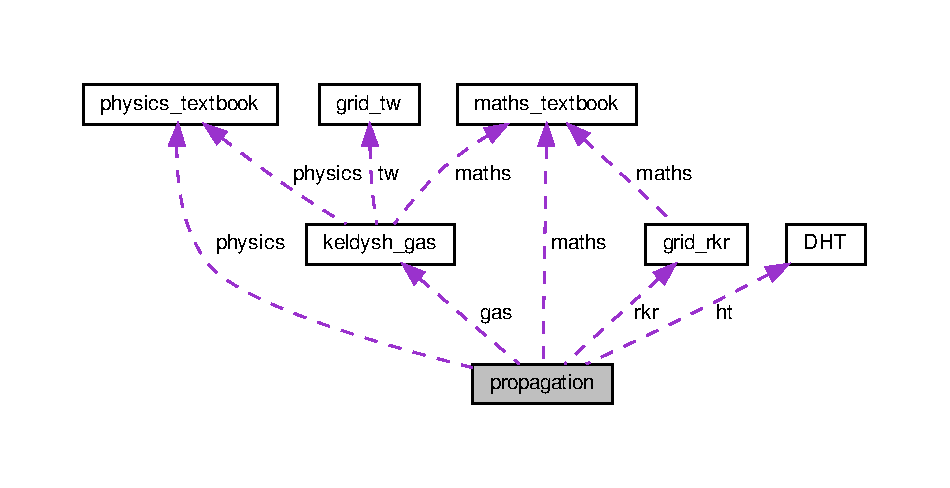
\includegraphics[width=345pt]{classpropagation__coll__graph}
\end{center}
\end{figure}
\subsection*{Public Member Functions}
\begin{DoxyCompactItemize}
\item 
\hyperlink{classpropagation_a9d7b9f42ce1c0bc741d3016a07ba13f7}{propagation} ()
\item 
\hyperlink{classpropagation_ab815c7ad4d93eaa7b7b821908fdc3203}{propagation} (double E\+\_\+min\+\_\+, Eigen\+::\+Array\+Xd w\+\_\+active\+\_\+, \hyperlink{classkeldysh__gas}{keldysh\+\_\+gas} \&gas\+\_\+, grid\+\_\+rkr \&rkr\+\_\+, \hyperlink{classphysics__textbook}{physics\+\_\+textbook} \&physics\+\_\+, \hyperlink{classmaths__textbook}{maths\+\_\+textbook} \&maths\+\_\+, D\+HT \&ht\+\_\+)
\item 
Eigen\+::\+Array\+Xd \hyperlink{classpropagation_a39126bbbd4977c140c0077b849e78bc1}{segment} (Eigen\+::\+Array\+Xd \hyperlink{classpropagation_a49a30e941421cd5e3f0b62bd1335a767}{k})
\item 
Eigen\+::\+Array\+X\+Xcd \hyperlink{classpropagation_af12b15d9b91f98516c0ff25efc1233d1}{block} (Eigen\+::\+Array\+X\+Xcd A\+\_\+w\+\_\+e\+\_\+)
\item 
std\+::complex$<$ double $>$ \hyperlink{classpropagation_a7c696d9e54e5f0a7735047e28aee4866}{n} (int i)
\item 
void \hyperlink{classpropagation_a65e272beb6b5b73f433456361bcde914}{near\+Field\+Propagation\+Step} (double dz, Eigen\+::\+Array\+X\+Xcd A\+\_\+w\+\_\+r\+\_\+)
\item 
void \hyperlink{classpropagation_a9c2e1cb4e314c173b26de08ffcfe071d}{far\+Field\+Propagation} ()
\end{DoxyCompactItemize}
\subsection*{Public Attributes}
\begin{DoxyCompactItemize}
\item 
double \hyperlink{classpropagation_aeacfc091fafd1fdb1af4536f6f587e55}{z}
\item 
int \hyperlink{classpropagation_a93033ee98c04a6fe007eae5c856e76b3}{n\+\_\+k}
\item 
Eigen\+::\+Array\+Xd \hyperlink{classpropagation_a4c24f42d4148eded469c6479d6bf1661}{w\+\_\+active}
\item 
Eigen\+::\+Array\+Xcd \hyperlink{classpropagation_a9e437271e452fa1732f50e006347b501}{k\+\_\+r}
\item 
Eigen\+::\+Array\+X\+Xcd \hyperlink{classpropagation_ad3a84addde67e43bbb606408193f78ee}{A\+\_\+w\+\_\+r}
\end{DoxyCompactItemize}
\subsection*{Private Attributes}
\begin{DoxyCompactItemize}
\item 
double \hyperlink{classpropagation_ab5a753d760a135806a93b9082e8019fb}{E\+\_\+min}
\item 
\hyperlink{classphysics__textbook}{physics\+\_\+textbook} \hyperlink{classpropagation_a42a6e725e3dd53cf94192bf93c31c8de}{physics}
\item 
\hyperlink{classmaths__textbook}{maths\+\_\+textbook} \hyperlink{classpropagation_ab5a5024c2d06c0dad06c745af7c6416c}{maths}
\item 
\hyperlink{classkeldysh__gas}{keldysh\+\_\+gas} \hyperlink{classpropagation_a4152dc9a226a7ff91aff2338d0bd813f}{gas}
\item 
grid\+\_\+rkr \hyperlink{classpropagation_a3d37531bb5918f972544d242aec7e72b}{rkr}
\item 
D\+HT \hyperlink{classpropagation_a044544975e7fc2ec3df9a55d92f8cc90}{ht}
\item 
Eigen\+::\+Array\+Xd \hyperlink{classpropagation_a07a80b67a345e3e9d8e934d2265ba288}{w\+\_\+active\+\_\+tmp}
\item 
int \hyperlink{classpropagation_a76f3651eac23a69c1259dc0406fbe0d9}{k\+\_\+excluded}
\item 
Eigen\+::\+Array\+Xcd \hyperlink{classpropagation_a49a30e941421cd5e3f0b62bd1335a767}{k}
\item 
Eigen\+::\+Array\+Xcd \hyperlink{classpropagation_aba601a0df3c63b13215c55d8ade2bcd7}{refractive\+Index}
\item 
Eigen\+::\+Array\+Xcd \hyperlink{classpropagation_a5ae0154dc8db04188ba92e10ba981000}{lamda}
\item 
Eigen\+::\+Array\+Xcd \hyperlink{classpropagation_a4df23dd19a8cca8a4cb032718dc2b258}{A\+\_\+w\+\_\+kr}
\item 
std\+::string \hyperlink{classpropagation_abd78bf6976f2b2d0a3fc82b9cf0d9dc6}{E\+\_\+f1\+\_\+f2\+\_\+data\+\_\+path}
\item 
Eigen\+::\+Array\+X\+Xd \hyperlink{classpropagation_a53ab4838e0e66b55c2ab1398389a22f5}{E\+\_\+f1\+\_\+f2\+\_\+data}
\item 
Eigen\+::\+Array\+Xd \hyperlink{classpropagation_aff3713e9170542e31c952a2d1b760eec}{E}
\item 
Eigen\+::\+Array\+Xd \hyperlink{classpropagation_a747dcaf8f7405a17af992bae39b7fab5}{f2}
\item 
Eigen\+::\+Array\+Xd \hyperlink{classpropagation_a14d6e72396c1c354c6d9986f2d79f85f}{f1}
\end{DoxyCompactItemize}


\subsection{Constructor \& Destructor Documentation}
\mbox{\Hypertarget{classpropagation_a9d7b9f42ce1c0bc741d3016a07ba13f7}\label{classpropagation_a9d7b9f42ce1c0bc741d3016a07ba13f7}} 
\index{propagation@{propagation}!propagation@{propagation}}
\index{propagation@{propagation}!propagation@{propagation}}
\subsubsection{\texorpdfstring{propagation()}{propagation()}\hspace{0.1cm}{\footnotesize\ttfamily [1/2]}}
{\footnotesize\ttfamily propagation\+::propagation (\begin{DoxyParamCaption}{ }\end{DoxyParamCaption})}

Constructor \mbox{\Hypertarget{classpropagation_ab815c7ad4d93eaa7b7b821908fdc3203}\label{classpropagation_ab815c7ad4d93eaa7b7b821908fdc3203}} 
\index{propagation@{propagation}!propagation@{propagation}}
\index{propagation@{propagation}!propagation@{propagation}}
\subsubsection{\texorpdfstring{propagation()}{propagation()}\hspace{0.1cm}{\footnotesize\ttfamily [2/2]}}
{\footnotesize\ttfamily propagation\+::propagation (\begin{DoxyParamCaption}\item[{double}]{E\+\_\+min\+\_\+,  }\item[{Eigen\+::\+Array\+Xd}]{w\+\_\+active\+\_\+,  }\item[{\hyperlink{classkeldysh__gas}{keldysh\+\_\+gas} \&}]{gas\+\_\+,  }\item[{grid\+\_\+rkr \&}]{rkr\+\_\+,  }\item[{\hyperlink{classphysics__textbook}{physics\+\_\+textbook} \&}]{physics\+\_\+,  }\item[{\hyperlink{classmaths__textbook}{maths\+\_\+textbook} \&}]{maths\+\_\+,  }\item[{D\+HT \&}]{ht\+\_\+ }\end{DoxyParamCaption})}



\subsection{Member Function Documentation}
\mbox{\Hypertarget{classpropagation_af12b15d9b91f98516c0ff25efc1233d1}\label{classpropagation_af12b15d9b91f98516c0ff25efc1233d1}} 
\index{propagation@{propagation}!block@{block}}
\index{block@{block}!propagation@{propagation}}
\subsubsection{\texorpdfstring{block()}{block()}}
{\footnotesize\ttfamily Eigen\+::\+Array\+X\+Xcd propagation\+::block (\begin{DoxyParamCaption}\item[{Eigen\+::\+Array\+X\+Xcd}]{A\+\_\+w\+\_\+e\+\_\+ }\end{DoxyParamCaption})}

\mbox{\Hypertarget{classpropagation_a9c2e1cb4e314c173b26de08ffcfe071d}\label{classpropagation_a9c2e1cb4e314c173b26de08ffcfe071d}} 
\index{propagation@{propagation}!far\+Field\+Propagation@{far\+Field\+Propagation}}
\index{far\+Field\+Propagation@{far\+Field\+Propagation}!propagation@{propagation}}
\subsubsection{\texorpdfstring{far\+Field\+Propagation()}{farFieldPropagation()}}
{\footnotesize\ttfamily void propagation\+::far\+Field\+Propagation (\begin{DoxyParamCaption}{ }\end{DoxyParamCaption})}

Fraunhofer diffraction for propagating into the far-\/field. \mbox{\Hypertarget{classpropagation_a7c696d9e54e5f0a7735047e28aee4866}\label{classpropagation_a7c696d9e54e5f0a7735047e28aee4866}} 
\index{propagation@{propagation}!n@{n}}
\index{n@{n}!propagation@{propagation}}
\subsubsection{\texorpdfstring{n()}{n()}}
{\footnotesize\ttfamily std\+::complex$<$ double $>$ propagation\+::n (\begin{DoxyParamCaption}\item[{int}]{i }\end{DoxyParamCaption})}

\mbox{\Hypertarget{classpropagation_a65e272beb6b5b73f433456361bcde914}\label{classpropagation_a65e272beb6b5b73f433456361bcde914}} 
\index{propagation@{propagation}!near\+Field\+Propagation\+Step@{near\+Field\+Propagation\+Step}}
\index{near\+Field\+Propagation\+Step@{near\+Field\+Propagation\+Step}!propagation@{propagation}}
\subsubsection{\texorpdfstring{near\+Field\+Propagation\+Step()}{nearFieldPropagationStep()}}
{\footnotesize\ttfamily void propagation\+::near\+Field\+Propagation\+Step (\begin{DoxyParamCaption}\item[{double}]{dz,  }\item[{Eigen\+::\+Array\+X\+Xcd}]{A\+\_\+w\+\_\+r\+\_\+ }\end{DoxyParamCaption})}

Angular Spectrum Method (A\+SM) for propagating in the near-\/field, in the gas-\/filled capillary. \mbox{[}Need to add citation!\mbox{]} For circularly-\/symmetric geometry\+: \[ E(z, r) = \mathcal{H}^{-1}\left(\mathcal{H}(E(0, r)) \times \exp(iz\sqrt{k^2 - k_r^2})\right). \] \mbox{\Hypertarget{classpropagation_a39126bbbd4977c140c0077b849e78bc1}\label{classpropagation_a39126bbbd4977c140c0077b849e78bc1}} 
\index{propagation@{propagation}!segment@{segment}}
\index{segment@{segment}!propagation@{propagation}}
\subsubsection{\texorpdfstring{segment()}{segment()}}
{\footnotesize\ttfamily Eigen\+::\+Array\+Xd propagation\+::segment (\begin{DoxyParamCaption}\item[{Eigen\+::\+Array\+Xd}]{k }\end{DoxyParamCaption})}



\subsection{Member Data Documentation}
\mbox{\Hypertarget{classpropagation_a4df23dd19a8cca8a4cb032718dc2b258}\label{classpropagation_a4df23dd19a8cca8a4cb032718dc2b258}} 
\index{propagation@{propagation}!A\+\_\+w\+\_\+kr@{A\+\_\+w\+\_\+kr}}
\index{A\+\_\+w\+\_\+kr@{A\+\_\+w\+\_\+kr}!propagation@{propagation}}
\subsubsection{\texorpdfstring{A\+\_\+w\+\_\+kr}{A\_w\_kr}}
{\footnotesize\ttfamily Eigen\+::\+Array\+Xcd propagation\+::\+A\+\_\+w\+\_\+kr\hspace{0.3cm}{\ttfamily [private]}}

\mbox{\Hypertarget{classpropagation_ad3a84addde67e43bbb606408193f78ee}\label{classpropagation_ad3a84addde67e43bbb606408193f78ee}} 
\index{propagation@{propagation}!A\+\_\+w\+\_\+r@{A\+\_\+w\+\_\+r}}
\index{A\+\_\+w\+\_\+r@{A\+\_\+w\+\_\+r}!propagation@{propagation}}
\subsubsection{\texorpdfstring{A\+\_\+w\+\_\+r}{A\_w\_r}}
{\footnotesize\ttfamily Eigen\+::\+Array\+X\+Xcd propagation\+::\+A\+\_\+w\+\_\+r}

\mbox{\Hypertarget{classpropagation_aff3713e9170542e31c952a2d1b760eec}\label{classpropagation_aff3713e9170542e31c952a2d1b760eec}} 
\index{propagation@{propagation}!E@{E}}
\index{E@{E}!propagation@{propagation}}
\subsubsection{\texorpdfstring{E}{E}}
{\footnotesize\ttfamily Eigen\+::\+Array\+Xd propagation\+::E\hspace{0.3cm}{\ttfamily [private]}}

\mbox{\Hypertarget{classpropagation_a53ab4838e0e66b55c2ab1398389a22f5}\label{classpropagation_a53ab4838e0e66b55c2ab1398389a22f5}} 
\index{propagation@{propagation}!E\+\_\+f1\+\_\+f2\+\_\+data@{E\+\_\+f1\+\_\+f2\+\_\+data}}
\index{E\+\_\+f1\+\_\+f2\+\_\+data@{E\+\_\+f1\+\_\+f2\+\_\+data}!propagation@{propagation}}
\subsubsection{\texorpdfstring{E\+\_\+f1\+\_\+f2\+\_\+data}{E\_f1\_f2\_data}}
{\footnotesize\ttfamily Eigen\+::\+Array\+X\+Xd propagation\+::\+E\+\_\+f1\+\_\+f2\+\_\+data\hspace{0.3cm}{\ttfamily [private]}}

\mbox{\Hypertarget{classpropagation_abd78bf6976f2b2d0a3fc82b9cf0d9dc6}\label{classpropagation_abd78bf6976f2b2d0a3fc82b9cf0d9dc6}} 
\index{propagation@{propagation}!E\+\_\+f1\+\_\+f2\+\_\+data\+\_\+path@{E\+\_\+f1\+\_\+f2\+\_\+data\+\_\+path}}
\index{E\+\_\+f1\+\_\+f2\+\_\+data\+\_\+path@{E\+\_\+f1\+\_\+f2\+\_\+data\+\_\+path}!propagation@{propagation}}
\subsubsection{\texorpdfstring{E\+\_\+f1\+\_\+f2\+\_\+data\+\_\+path}{E\_f1\_f2\_data\_path}}
{\footnotesize\ttfamily std\+::string propagation\+::\+E\+\_\+f1\+\_\+f2\+\_\+data\+\_\+path\hspace{0.3cm}{\ttfamily [private]}}

\mbox{\Hypertarget{classpropagation_ab5a753d760a135806a93b9082e8019fb}\label{classpropagation_ab5a753d760a135806a93b9082e8019fb}} 
\index{propagation@{propagation}!E\+\_\+min@{E\+\_\+min}}
\index{E\+\_\+min@{E\+\_\+min}!propagation@{propagation}}
\subsubsection{\texorpdfstring{E\+\_\+min}{E\_min}}
{\footnotesize\ttfamily double propagation\+::\+E\+\_\+min\hspace{0.3cm}{\ttfamily [private]}}

\mbox{\Hypertarget{classpropagation_a14d6e72396c1c354c6d9986f2d79f85f}\label{classpropagation_a14d6e72396c1c354c6d9986f2d79f85f}} 
\index{propagation@{propagation}!f1@{f1}}
\index{f1@{f1}!propagation@{propagation}}
\subsubsection{\texorpdfstring{f1}{f1}}
{\footnotesize\ttfamily Eigen\+::\+Array\+Xd propagation\+::f1\hspace{0.3cm}{\ttfamily [private]}}

\mbox{\Hypertarget{classpropagation_a747dcaf8f7405a17af992bae39b7fab5}\label{classpropagation_a747dcaf8f7405a17af992bae39b7fab5}} 
\index{propagation@{propagation}!f2@{f2}}
\index{f2@{f2}!propagation@{propagation}}
\subsubsection{\texorpdfstring{f2}{f2}}
{\footnotesize\ttfamily Eigen\+::\+Array\+Xd propagation\+::f2\hspace{0.3cm}{\ttfamily [private]}}

\mbox{\Hypertarget{classpropagation_a4152dc9a226a7ff91aff2338d0bd813f}\label{classpropagation_a4152dc9a226a7ff91aff2338d0bd813f}} 
\index{propagation@{propagation}!gas@{gas}}
\index{gas@{gas}!propagation@{propagation}}
\subsubsection{\texorpdfstring{gas}{gas}}
{\footnotesize\ttfamily \hyperlink{classkeldysh__gas}{keldysh\+\_\+gas} propagation\+::gas\hspace{0.3cm}{\ttfamily [private]}}

\mbox{\Hypertarget{classpropagation_a044544975e7fc2ec3df9a55d92f8cc90}\label{classpropagation_a044544975e7fc2ec3df9a55d92f8cc90}} 
\index{propagation@{propagation}!ht@{ht}}
\index{ht@{ht}!propagation@{propagation}}
\subsubsection{\texorpdfstring{ht}{ht}}
{\footnotesize\ttfamily D\+HT propagation\+::ht\hspace{0.3cm}{\ttfamily [private]}}

Hankel transform \mbox{\Hypertarget{classpropagation_a49a30e941421cd5e3f0b62bd1335a767}\label{classpropagation_a49a30e941421cd5e3f0b62bd1335a767}} 
\index{propagation@{propagation}!k@{k}}
\index{k@{k}!propagation@{propagation}}
\subsubsection{\texorpdfstring{k}{k}}
{\footnotesize\ttfamily Eigen\+::\+Array\+Xcd propagation\+::k\hspace{0.3cm}{\ttfamily [private]}}

\mbox{\Hypertarget{classpropagation_a76f3651eac23a69c1259dc0406fbe0d9}\label{classpropagation_a76f3651eac23a69c1259dc0406fbe0d9}} 
\index{propagation@{propagation}!k\+\_\+excluded@{k\+\_\+excluded}}
\index{k\+\_\+excluded@{k\+\_\+excluded}!propagation@{propagation}}
\subsubsection{\texorpdfstring{k\+\_\+excluded}{k\_excluded}}
{\footnotesize\ttfamily int propagation\+::k\+\_\+excluded\hspace{0.3cm}{\ttfamily [private]}}

\mbox{\Hypertarget{classpropagation_a9e437271e452fa1732f50e006347b501}\label{classpropagation_a9e437271e452fa1732f50e006347b501}} 
\index{propagation@{propagation}!k\+\_\+r@{k\+\_\+r}}
\index{k\+\_\+r@{k\+\_\+r}!propagation@{propagation}}
\subsubsection{\texorpdfstring{k\+\_\+r}{k\_r}}
{\footnotesize\ttfamily Eigen\+::\+Array\+Xcd propagation\+::k\+\_\+r}

\mbox{\Hypertarget{classpropagation_a5ae0154dc8db04188ba92e10ba981000}\label{classpropagation_a5ae0154dc8db04188ba92e10ba981000}} 
\index{propagation@{propagation}!lamda@{lamda}}
\index{lamda@{lamda}!propagation@{propagation}}
\subsubsection{\texorpdfstring{lamda}{lamda}}
{\footnotesize\ttfamily Eigen\+::\+Array\+Xcd propagation\+::lamda\hspace{0.3cm}{\ttfamily [private]}}

\mbox{\Hypertarget{classpropagation_ab5a5024c2d06c0dad06c745af7c6416c}\label{classpropagation_ab5a5024c2d06c0dad06c745af7c6416c}} 
\index{propagation@{propagation}!maths@{maths}}
\index{maths@{maths}!propagation@{propagation}}
\subsubsection{\texorpdfstring{maths}{maths}}
{\footnotesize\ttfamily \hyperlink{classmaths__textbook}{maths\+\_\+textbook} propagation\+::maths\hspace{0.3cm}{\ttfamily [private]}}

Mathematical constants and functions \mbox{\Hypertarget{classpropagation_a93033ee98c04a6fe007eae5c856e76b3}\label{classpropagation_a93033ee98c04a6fe007eae5c856e76b3}} 
\index{propagation@{propagation}!n\+\_\+k@{n\+\_\+k}}
\index{n\+\_\+k@{n\+\_\+k}!propagation@{propagation}}
\subsubsection{\texorpdfstring{n\+\_\+k}{n\_k}}
{\footnotesize\ttfamily int propagation\+::n\+\_\+k}

\mbox{\Hypertarget{classpropagation_a42a6e725e3dd53cf94192bf93c31c8de}\label{classpropagation_a42a6e725e3dd53cf94192bf93c31c8de}} 
\index{propagation@{propagation}!physics@{physics}}
\index{physics@{physics}!propagation@{propagation}}
\subsubsection{\texorpdfstring{physics}{physics}}
{\footnotesize\ttfamily \hyperlink{classphysics__textbook}{physics\+\_\+textbook} propagation\+::physics\hspace{0.3cm}{\ttfamily [private]}}

Physical constants \mbox{\Hypertarget{classpropagation_aba601a0df3c63b13215c55d8ade2bcd7}\label{classpropagation_aba601a0df3c63b13215c55d8ade2bcd7}} 
\index{propagation@{propagation}!refractive\+Index@{refractive\+Index}}
\index{refractive\+Index@{refractive\+Index}!propagation@{propagation}}
\subsubsection{\texorpdfstring{refractive\+Index}{refractiveIndex}}
{\footnotesize\ttfamily Eigen\+::\+Array\+Xcd propagation\+::refractive\+Index\hspace{0.3cm}{\ttfamily [private]}}

\mbox{\Hypertarget{classpropagation_a3d37531bb5918f972544d242aec7e72b}\label{classpropagation_a3d37531bb5918f972544d242aec7e72b}} 
\index{propagation@{propagation}!rkr@{rkr}}
\index{rkr@{rkr}!propagation@{propagation}}
\subsubsection{\texorpdfstring{rkr}{rkr}}
{\footnotesize\ttfamily grid\+\_\+rkr propagation\+::rkr\hspace{0.3cm}{\ttfamily [private]}}

Radial grid \mbox{\Hypertarget{classpropagation_a4c24f42d4148eded469c6479d6bf1661}\label{classpropagation_a4c24f42d4148eded469c6479d6bf1661}} 
\index{propagation@{propagation}!w\+\_\+active@{w\+\_\+active}}
\index{w\+\_\+active@{w\+\_\+active}!propagation@{propagation}}
\subsubsection{\texorpdfstring{w\+\_\+active}{w\_active}}
{\footnotesize\ttfamily Eigen\+::\+Array\+Xd propagation\+::w\+\_\+active}

\mbox{\Hypertarget{classpropagation_a07a80b67a345e3e9d8e934d2265ba288}\label{classpropagation_a07a80b67a345e3e9d8e934d2265ba288}} 
\index{propagation@{propagation}!w\+\_\+active\+\_\+tmp@{w\+\_\+active\+\_\+tmp}}
\index{w\+\_\+active\+\_\+tmp@{w\+\_\+active\+\_\+tmp}!propagation@{propagation}}
\subsubsection{\texorpdfstring{w\+\_\+active\+\_\+tmp}{w\_active\_tmp}}
{\footnotesize\ttfamily Eigen\+::\+Array\+Xd propagation\+::w\+\_\+active\+\_\+tmp\hspace{0.3cm}{\ttfamily [private]}}

\mbox{\Hypertarget{classpropagation_aeacfc091fafd1fdb1af4536f6f587e55}\label{classpropagation_aeacfc091fafd1fdb1af4536f6f587e55}} 
\index{propagation@{propagation}!z@{z}}
\index{z@{z}!propagation@{propagation}}
\subsubsection{\texorpdfstring{z}{z}}
{\footnotesize\ttfamily double propagation\+::z}



The documentation for this class was generated from the following files\+:\begin{DoxyCompactItemize}
\item 
/home/sam/\+Project/\+X\+N\+L\+O/\+H\+H\+G\+P/src/\hyperlink{propagation_8hpp}{propagation.\+hpp}\item 
/home/sam/\+Project/\+X\+N\+L\+O/\+H\+H\+G\+P/src/\hyperlink{propagation_8cpp}{propagation.\+cpp}\end{DoxyCompactItemize}

\chapter{File Documentation}
\hypertarget{_d_h_t_8cpp}{}\section{/\+Users/sms1n16/\+Project/\+X\+N\+L\+O/src/\+D\+H\+T/\+D\+HT.cpp File Reference}
\label{_d_h_t_8cpp}\index{/Users/sms1n16/Project/XNLO/src/DHT/DHT.cpp@{/Users/sms1n16/Project/XNLO/src/DHT/DHT.cpp}}
{\ttfamily \#include \char`\"{}D\+H\+T.\+hpp\char`\"{}}\newline
{\ttfamily \#include \char`\"{}../../\+Eigen/\+Dense\char`\"{}}\newline
{\ttfamily \#include \char`\"{}../maths/maths\+\_\+textbook.\+hpp\char`\"{}}\newline

\hypertarget{_d_h_t_8hpp}{}\section{/home/sam/\+Project/\+X\+N\+L\+O/src/\+D\+H\+T/\+D\+HT.hpp File Reference}
\label{_d_h_t_8hpp}\index{/home/sam/Project/XNLO/src/DHT/DHT.hpp@{/home/sam/Project/XNLO/src/DHT/DHT.hpp}}
{\ttfamily \#include \char`\"{}../../\+Eigen/\+Dense\char`\"{}}\newline
{\ttfamily \#include \char`\"{}../maths/maths\+\_\+textbook.\+hpp\char`\"{}}\newline
Include dependency graph for D\+H\+T.\+hpp\+:
\nopagebreak
\begin{figure}[H]
\begin{center}
\leavevmode
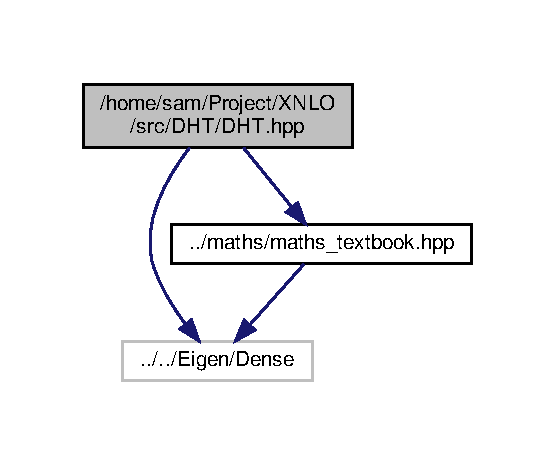
\includegraphics[width=267pt]{_d_h_t_8hpp__incl}
\end{center}
\end{figure}
This graph shows which files directly or indirectly include this file\+:
\nopagebreak
\begin{figure}[H]
\begin{center}
\leavevmode
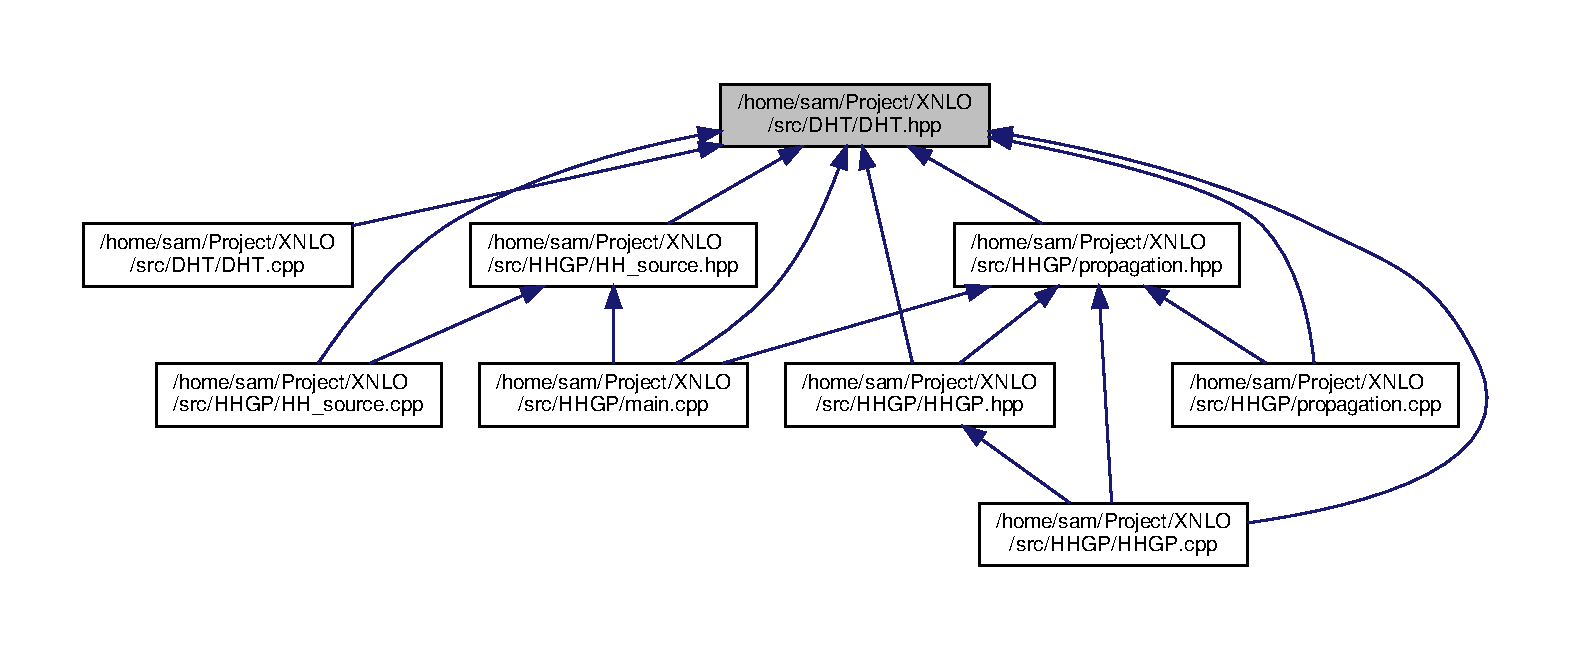
\includegraphics[width=350pt]{_d_h_t_8hpp__dep__incl}
\end{center}
\end{figure}
\subsection*{Classes}
\begin{DoxyCompactItemize}
\item 
class \mbox{\hyperlink{class_d_h_t}{D\+HT}}
\end{DoxyCompactItemize}

\hypertarget{keldysh__gas_8cpp}{}\section{/\+Users/sms1n16/\+Project/\+X\+N\+L\+O/src/gas/keldysh\+\_\+gas.cpp File Reference}
\label{keldysh__gas_8cpp}\index{/\+Users/sms1n16/\+Project/\+X\+N\+L\+O/src/gas/keldysh\+\_\+gas.\+cpp@{/\+Users/sms1n16/\+Project/\+X\+N\+L\+O/src/gas/keldysh\+\_\+gas.\+cpp}}
{\ttfamily \#include \char`\"{}keldysh\+\_\+gas.\+hpp\char`\"{}}\newline
{\ttfamily \#include \char`\"{}../physics/physics\+\_\+textbook.\+hpp\char`\"{}}\newline
{\ttfamily \#include \char`\"{}../grid/grid\+\_\+tw.\+hpp\char`\"{}}\newline
{\ttfamily \#include $<$mkl.\+h$>$}\newline
{\ttfamily \#include \char`\"{}../../\+Eigen/\+Dense\char`\"{}}\newline
{\ttfamily \#include \char`\"{}../maths/maths\+\_\+textbook.\+hpp\char`\"{}}\newline
{\ttfamily \#include $<$cmath$>$}\newline
{\ttfamily \#include $<$iostream$>$}\newline
Include dependency graph for keldysh\+\_\+gas.\+cpp\+:\nopagebreak
\begin{figure}[H]
\begin{center}
\leavevmode
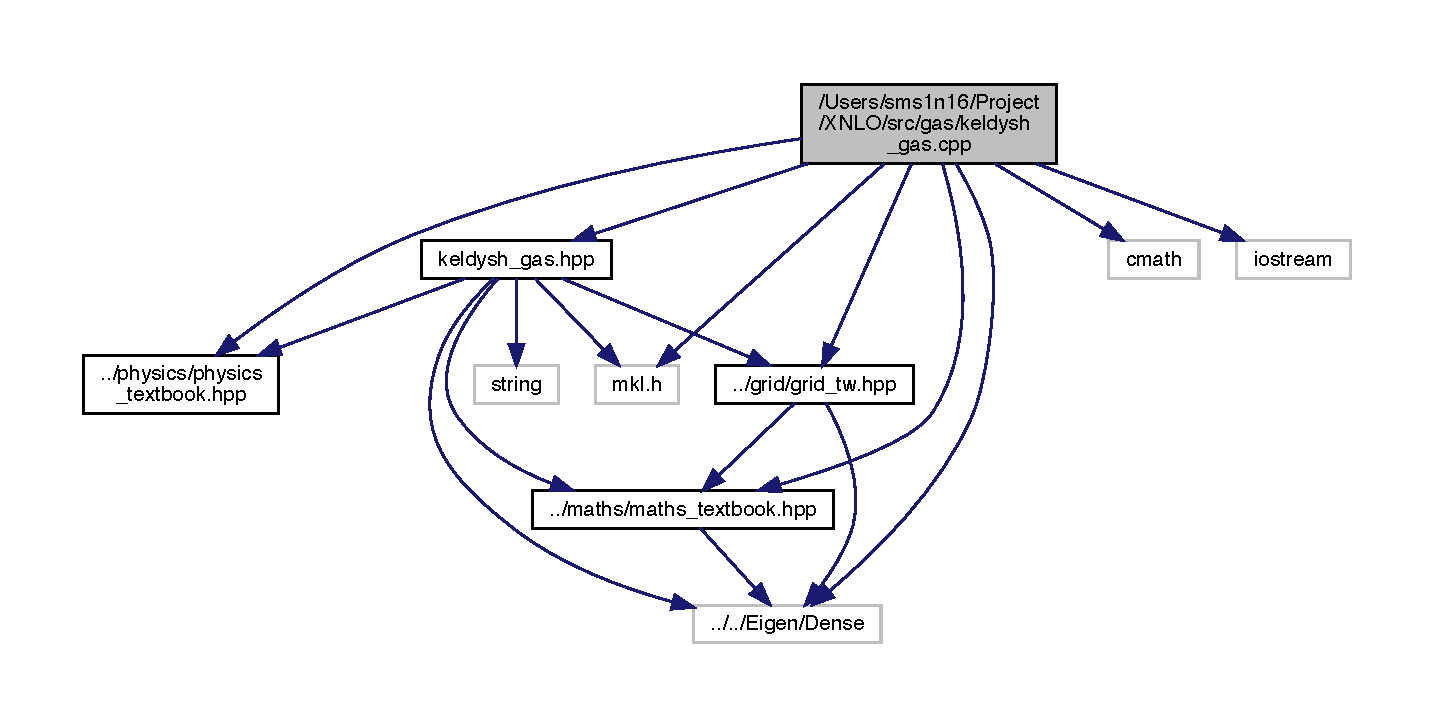
\includegraphics[width=350pt]{keldysh__gas_8cpp__incl}
\end{center}
\end{figure}

\hypertarget{keldysh__gas_8hpp}{}\section{/\+Users/sms1n16/\+Project/\+X\+N\+L\+O/src/gas/keldysh\+\_\+gas.hpp File Reference}
\label{keldysh__gas_8hpp}\index{/Users/sms1n16/Project/XNLO/src/gas/keldysh\_gas.hpp@{/Users/sms1n16/Project/XNLO/src/gas/keldysh\_gas.hpp}}
{\ttfamily \#include \char`\"{}../physics/physics\+\_\+textbook.\+hpp\char`\"{}}\newline
{\ttfamily \#include \char`\"{}../maths/maths\+\_\+textbook.\+hpp\char`\"{}}\newline
{\ttfamily \#include \char`\"{}../grid/grid\+\_\+tw.\+hpp\char`\"{}}\newline
{\ttfamily \#include $<$mkl.\+h$>$}\newline
{\ttfamily \#include \char`\"{}../../\+Eigen/\+Dense\char`\"{}}\newline
{\ttfamily \#include $<$string$>$}\newline
Include dependency graph for keldysh\+\_\+gas.\+hpp\+:\nopagebreak
\begin{figure}[H]
\begin{center}
\leavevmode
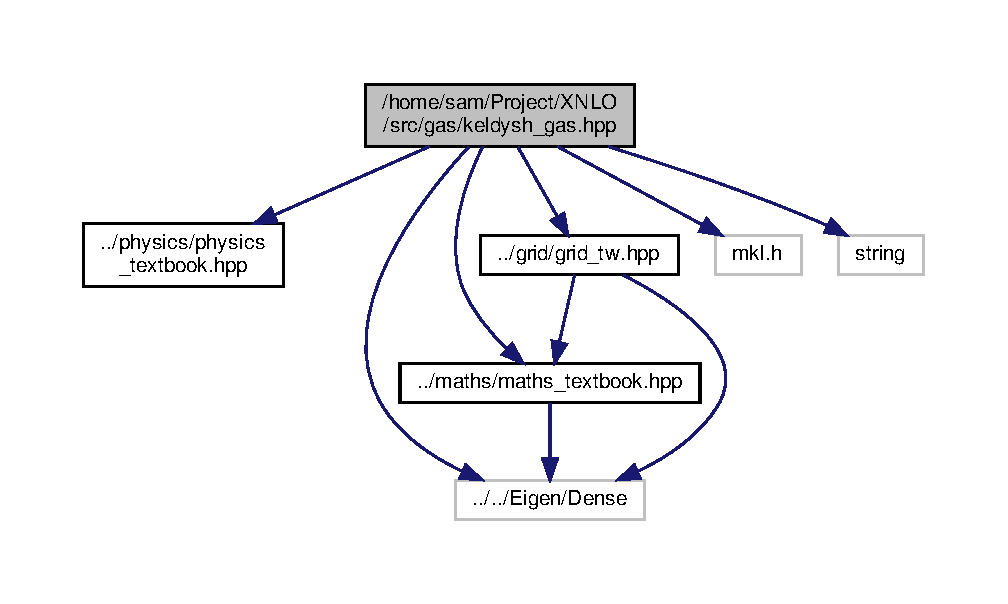
\includegraphics[width=350pt]{keldysh__gas_8hpp__incl}
\end{center}
\end{figure}
This graph shows which files directly or indirectly include this file\+:\nopagebreak
\begin{figure}[H]
\begin{center}
\leavevmode
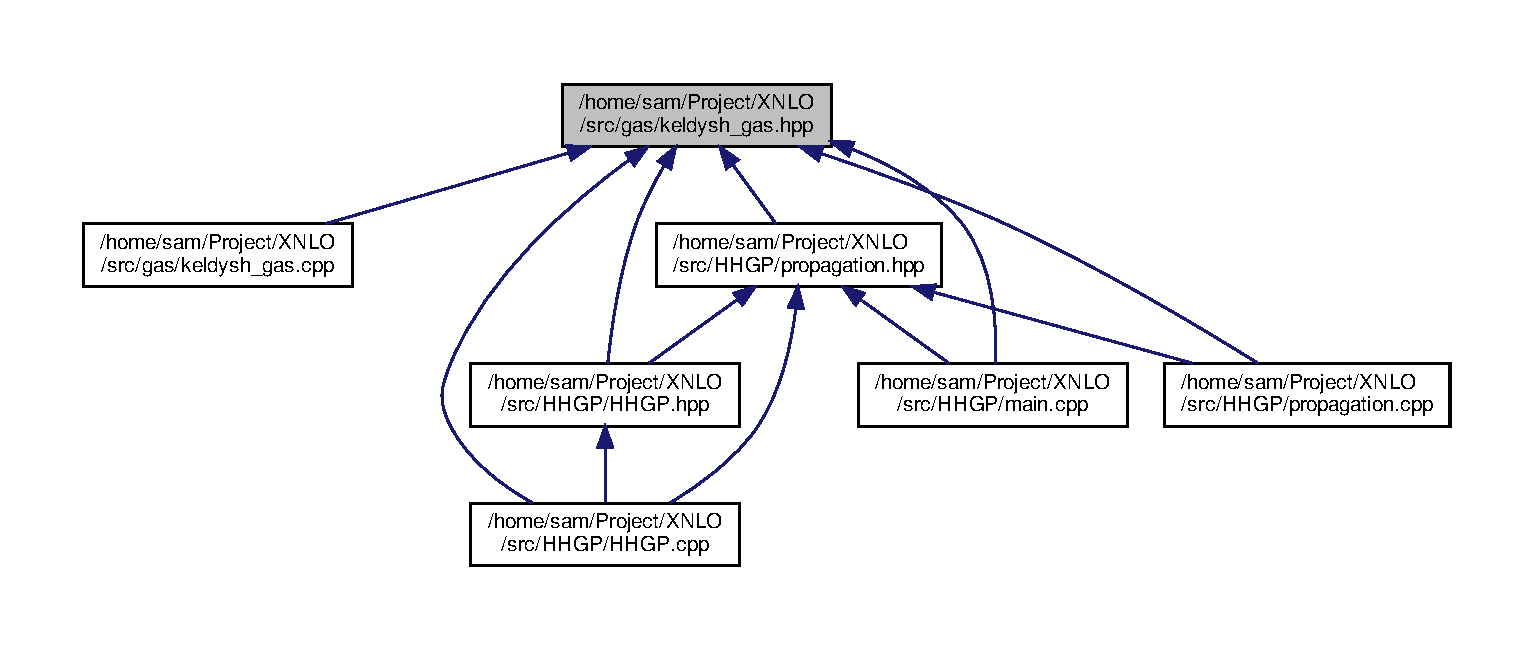
\includegraphics[width=350pt]{keldysh__gas_8hpp__dep__incl}
\end{center}
\end{figure}
\subsection*{Classes}
\begin{DoxyCompactItemize}
\item 
class \mbox{\hyperlink{classkeldysh__gas}{keldysh\+\_\+gas}}
\end{DoxyCompactItemize}

\hypertarget{grid__rkr_8cpp}{}\section{/home/sam/\+Project/\+X\+N\+L\+O/\+H\+H\+G\+P/src/grid\+\_\+rkr.cpp File Reference}
\label{grid__rkr_8cpp}\index{/home/sam/\+Project/\+X\+N\+L\+O/\+H\+H\+G\+P/src/grid\+\_\+rkr.\+cpp@{/home/sam/\+Project/\+X\+N\+L\+O/\+H\+H\+G\+P/src/grid\+\_\+rkr.\+cpp}}
{\ttfamily \#include \char`\"{}grid\+\_\+rkr.\+hpp\char`\"{}}\newline
{\ttfamily \#include \char`\"{}maths\+\_\+textbook.\+hpp\char`\"{}}\newline
{\ttfamily \#include \char`\"{}Eigen/\+Dense\char`\"{}}\newline
Include dependency graph for grid\+\_\+rkr.\+cpp\+:\nopagebreak
\begin{figure}[H]
\begin{center}
\leavevmode
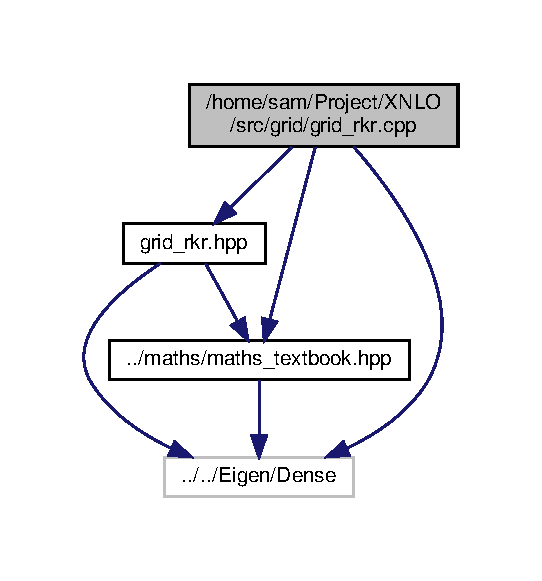
\includegraphics[width=251pt]{grid__rkr_8cpp__incl}
\end{center}
\end{figure}
\subsection*{Namespaces}
\begin{DoxyCompactItemize}
\item 
 \hyperlink{namespace_h_h_g_p}{H\+H\+GP}
\end{DoxyCompactItemize}

\hypertarget{grid__rkr_8hpp}{}\section{/home/sam/\+Project/\+X\+N\+L\+O/src/grid/grid\+\_\+rkr.hpp File Reference}
\label{grid__rkr_8hpp}\index{/home/sam/\+Project/\+X\+N\+L\+O/src/grid/grid\+\_\+rkr.\+hpp@{/home/sam/\+Project/\+X\+N\+L\+O/src/grid/grid\+\_\+rkr.\+hpp}}
{\ttfamily \#include \char`\"{}../../\+Eigen/\+Dense\char`\"{}}\newline
{\ttfamily \#include \char`\"{}../maths/maths\+\_\+textbook.\+hpp\char`\"{}}\newline
Include dependency graph for grid\+\_\+rkr.\+hpp\+:\nopagebreak
\begin{figure}[H]
\begin{center}
\leavevmode
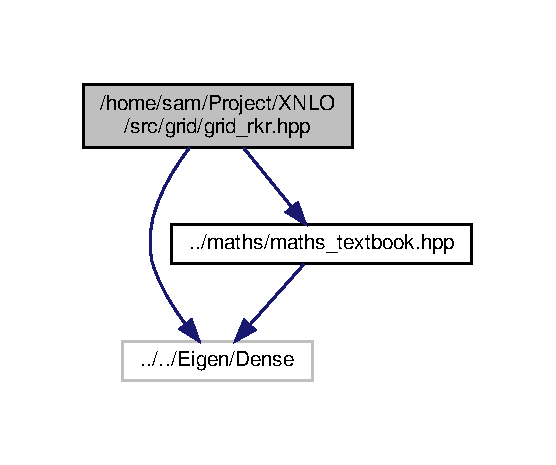
\includegraphics[width=267pt]{grid__rkr_8hpp__incl}
\end{center}
\end{figure}
This graph shows which files directly or indirectly include this file\+:\nopagebreak
\begin{figure}[H]
\begin{center}
\leavevmode
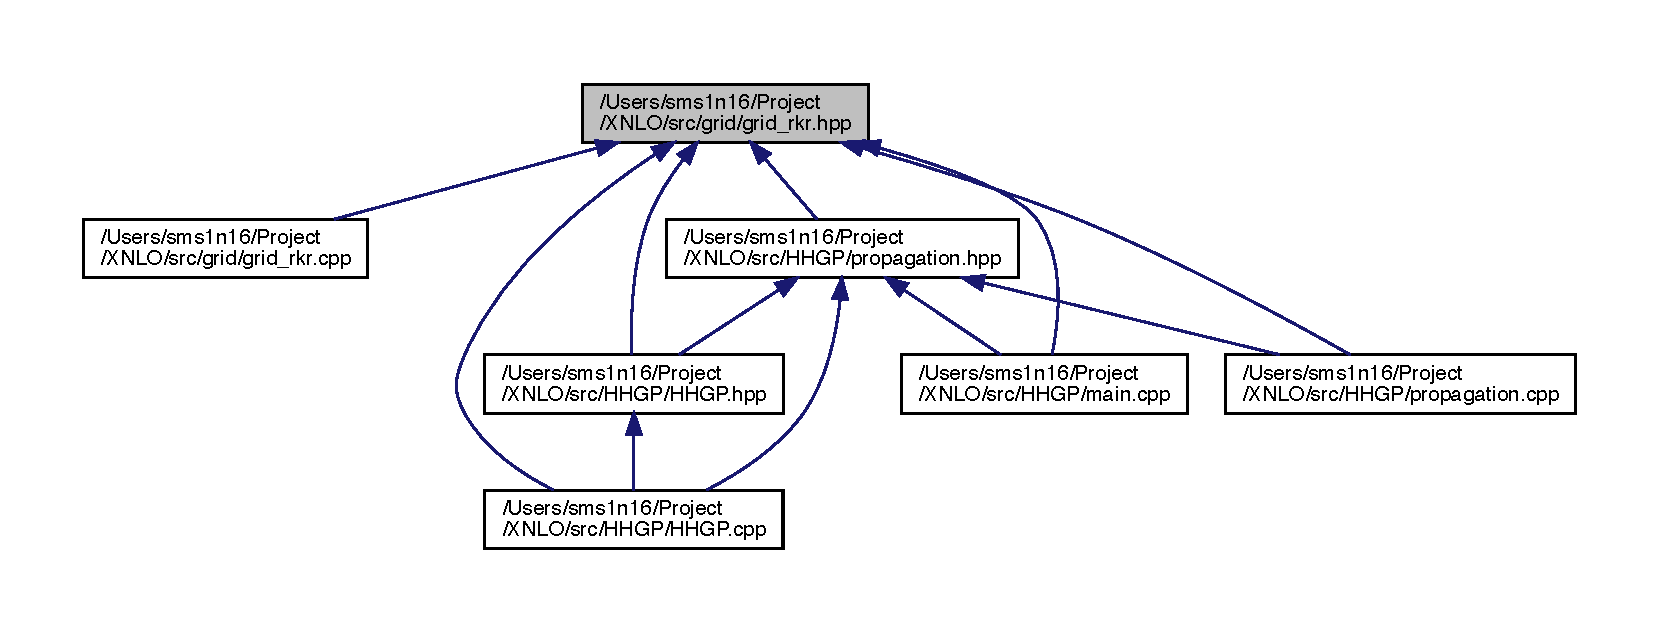
\includegraphics[width=350pt]{grid__rkr_8hpp__dep__incl}
\end{center}
\end{figure}
\subsection*{Classes}
\begin{DoxyCompactItemize}
\item 
class \hyperlink{classgrid__rkr}{grid\+\_\+rkr}
\end{DoxyCompactItemize}

\hypertarget{grid__tw_8cpp}{}\section{/\+Users/sms1n16/\+Project/\+X\+N\+L\+O/src/grid/grid\+\_\+tw.cpp File Reference}
\label{grid__tw_8cpp}\index{/Users/sms1n16/Project/XNLO/src/grid/grid\_tw.cpp@{/Users/sms1n16/Project/XNLO/src/grid/grid\_tw.cpp}}
{\ttfamily \#include \char`\"{}grid\+\_\+tw.\+hpp\char`\"{}}\newline
{\ttfamily \#include \char`\"{}../maths/maths\+\_\+textbook.\+hpp\char`\"{}}\newline
{\ttfamily \#include \char`\"{}../../\+Eigen/\+Dense\char`\"{}}\newline
{\ttfamily \#include $<$iostream$>$}\newline
Include dependency graph for grid\+\_\+tw.\+cpp\+:\nopagebreak
\begin{figure}[H]
\begin{center}
\leavevmode
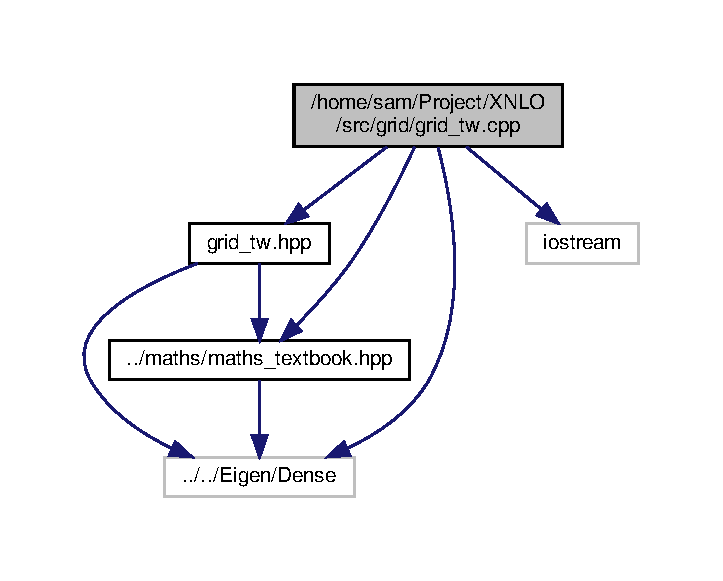
\includegraphics[width=347pt]{grid__tw_8cpp__incl}
\end{center}
\end{figure}
\subsection*{Namespaces}
\begin{DoxyCompactItemize}
\item 
 \mbox{\hyperlink{namespace_x_n_l_o}{X\+N\+LO}}
\end{DoxyCompactItemize}

\hypertarget{grid__tw_8hpp}{}\section{/\+Users/sms1n16/\+Project/\+X\+N\+L\+O/src/grid/grid\+\_\+tw.hpp File Reference}
\label{grid__tw_8hpp}\index{/Users/sms1n16/Project/XNLO/src/grid/grid\_tw.hpp@{/Users/sms1n16/Project/XNLO/src/grid/grid\_tw.hpp}}
{\ttfamily \#include \char`\"{}../../\+Eigen/\+Dense\char`\"{}}\newline
{\ttfamily \#include \char`\"{}../maths/maths\+\_\+textbook.\+hpp\char`\"{}}\newline
Include dependency graph for grid\+\_\+tw.\+hpp\+:\nopagebreak
\begin{figure}[H]
\begin{center}
\leavevmode
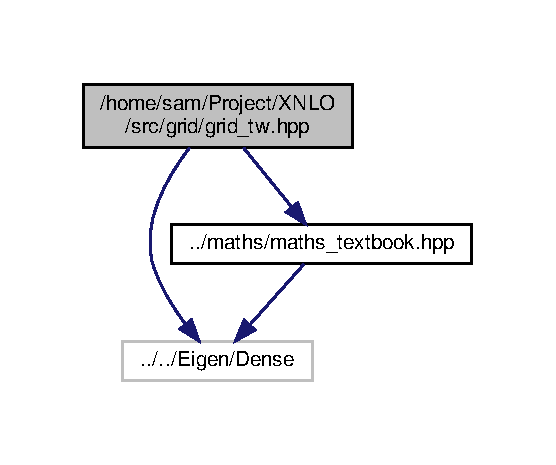
\includegraphics[width=270pt]{grid__tw_8hpp__incl}
\end{center}
\end{figure}
This graph shows which files directly or indirectly include this file\+:\nopagebreak
\begin{figure}[H]
\begin{center}
\leavevmode
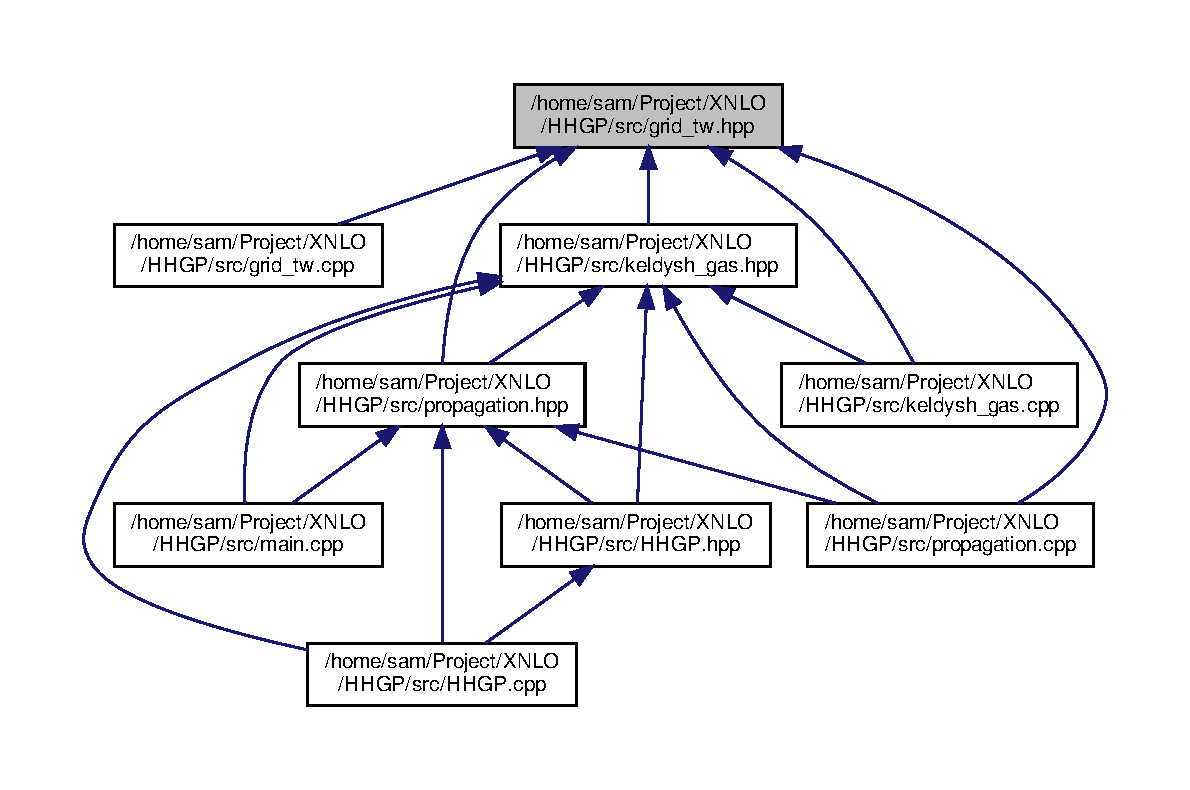
\includegraphics[width=350pt]{grid__tw_8hpp__dep__incl}
\end{center}
\end{figure}
\subsection*{Classes}
\begin{DoxyCompactItemize}
\item 
class \mbox{\hyperlink{classgrid__tw}{grid\+\_\+tw}}
\item 
class \mbox{\hyperlink{class_x_n_l_o_1_1grid__tw}{X\+N\+L\+O\+::grid\+\_\+tw}}
\end{DoxyCompactItemize}
\subsection*{Namespaces}
\begin{DoxyCompactItemize}
\item 
 \mbox{\hyperlink{namespace_x_n_l_o}{X\+N\+LO}}
\end{DoxyCompactItemize}

\input{grid__xkx_8cpp}
\input{grid__xkx_8hpp}
\hypertarget{config__settings_8cpp}{}\section{/\+Users/sms1n16/\+Project/\+X\+N\+L\+O/src/\+H\+H\+G\+P/config\+\_\+settings.cpp File Reference}
\label{config__settings_8cpp}\index{/\+Users/sms1n16/\+Project/\+X\+N\+L\+O/src/\+H\+H\+G\+P/config\+\_\+settings.\+cpp@{/\+Users/sms1n16/\+Project/\+X\+N\+L\+O/src/\+H\+H\+G\+P/config\+\_\+settings.\+cpp}}
{\ttfamily \#include \char`\"{}config\+\_\+settings.\+hpp\char`\"{}}\newline
{\ttfamily \#include $<$fstream$>$}\newline
{\ttfamily \#include $<$iostream$>$}\newline
{\ttfamily \#include $<$string$>$}\newline
Include dependency graph for config\+\_\+settings.\+cpp\+:\nopagebreak
\begin{figure}[H]
\begin{center}
\leavevmode
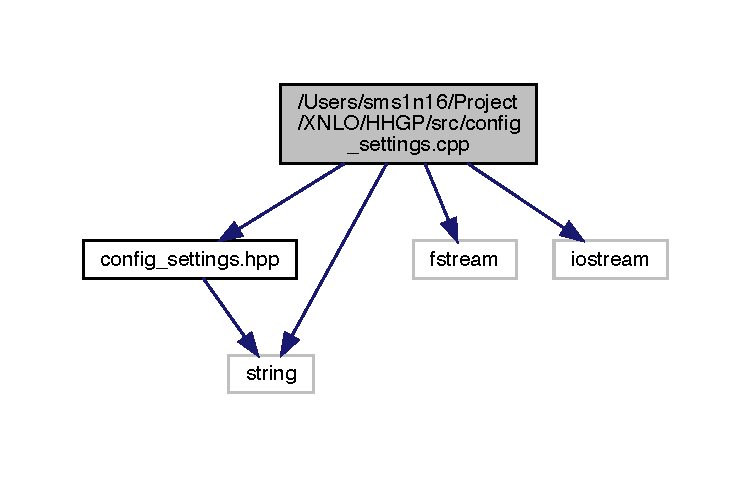
\includegraphics[width=350pt]{config__settings_8cpp__incl}
\end{center}
\end{figure}
\subsection*{Namespaces}
\begin{DoxyCompactItemize}
\item 
 \hyperlink{namespace_h_h}{HH}
\end{DoxyCompactItemize}

\hypertarget{config__settings_8hpp}{}\section{/\+Users/sms1n16/\+Project/\+X\+N\+L\+O/\+H\+H\+G\+P/src/config\+\_\+settings.hpp File Reference}
\label{config__settings_8hpp}\index{/\+Users/sms1n16/\+Project/\+X\+N\+L\+O/\+H\+H\+G\+P/src/config\+\_\+settings.\+hpp@{/\+Users/sms1n16/\+Project/\+X\+N\+L\+O/\+H\+H\+G\+P/src/config\+\_\+settings.\+hpp}}
{\ttfamily \#include $<$string$>$}\newline
Include dependency graph for config\+\_\+settings.\+hpp\+:\nopagebreak
\begin{figure}[H]
\begin{center}
\leavevmode
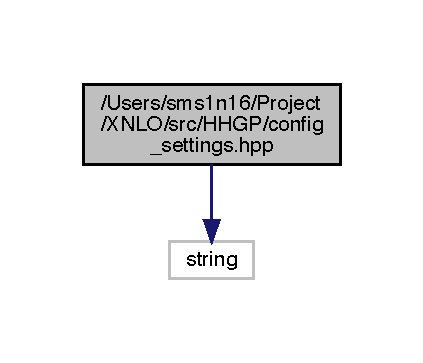
\includegraphics[width=203pt]{config__settings_8hpp__incl}
\end{center}
\end{figure}
This graph shows which files directly or indirectly include this file\+:\nopagebreak
\begin{figure}[H]
\begin{center}
\leavevmode
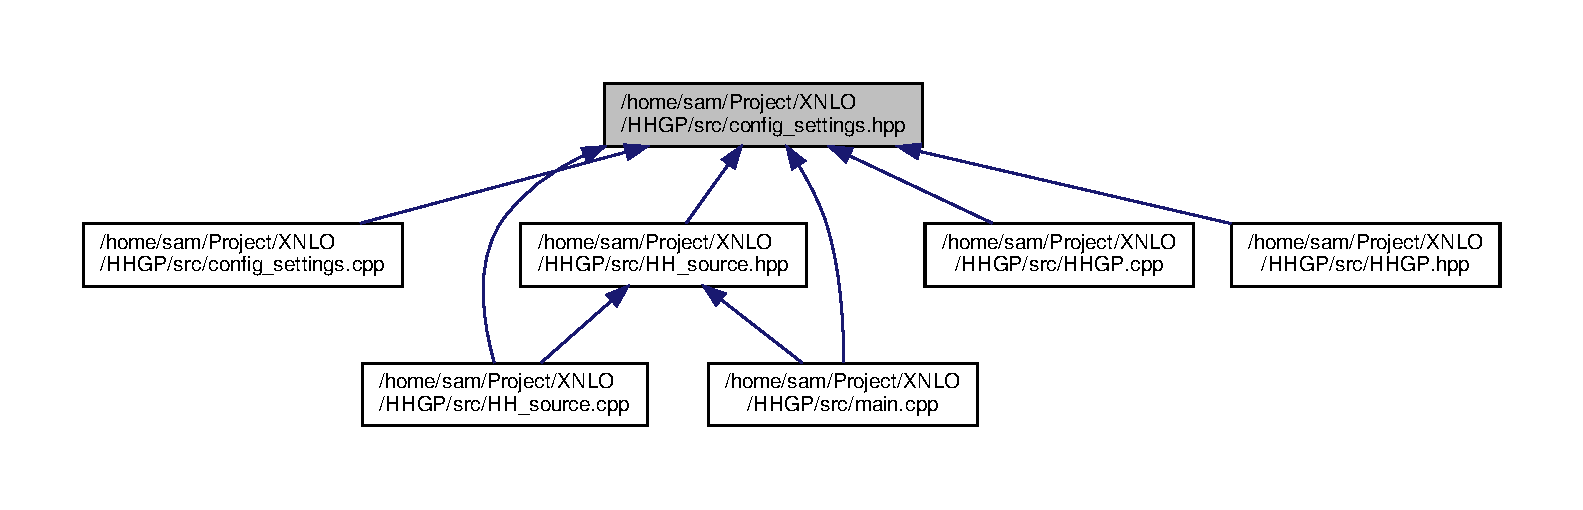
\includegraphics[width=350pt]{config__settings_8hpp__dep__incl}
\end{center}
\end{figure}
\subsection*{Classes}
\begin{DoxyCompactItemize}
\item 
class \hyperlink{class_config___settings}{Config\+\_\+\+Settings}
\end{DoxyCompactItemize}

\hypertarget{_h_h__source_8cpp}{}\section{/home/sam/\+Project/\+X\+N\+L\+O/\+H\+H\+G\+P/src/\+H\+H\+\_\+source.cpp File Reference}
\label{_h_h__source_8cpp}\index{/home/sam/\+Project/\+X\+N\+L\+O/\+H\+H\+G\+P/src/\+H\+H\+\_\+source.\+cpp@{/home/sam/\+Project/\+X\+N\+L\+O/\+H\+H\+G\+P/src/\+H\+H\+\_\+source.\+cpp}}
{\ttfamily \#include $<$iostream$>$}\newline
{\ttfamily \#include $<$string$>$}\newline
{\ttfamily \#include \char`\"{}Eigen/\+Dense\char`\"{}}\newline
{\ttfamily \#include \char`\"{}H\+H\+\_\+source.\+hpp\char`\"{}}\newline
{\ttfamily \#include \char`\"{}../../src/\+I\+O.\+hpp\char`\"{}}\newline
{\ttfamily \#include \char`\"{}config\+\_\+settings.\+hpp\char`\"{}}\newline
{\ttfamily \#include \char`\"{}../../src/maths\+\_\+textbook.\+hpp\char`\"{}}\newline
{\ttfamily \#include \char`\"{}../../src/\+D\+H\+T.\+hpp\char`\"{}}\newline

\hypertarget{_h_h__source_8hpp}{}\section{/home/sam/\+Project/\+X\+N\+L\+O/src/\+H\+H\+G\+P/\+H\+H\+\_\+source.hpp File Reference}
\label{_h_h__source_8hpp}\index{/home/sam/Project/XNLO/src/HHGP/HH\_source.hpp@{/home/sam/Project/XNLO/src/HHGP/HH\_source.hpp}}
{\ttfamily \#include $<$iostream$>$}\newline
{\ttfamily \#include $<$string$>$}\newline
{\ttfamily \#include \char`\"{}../../\+Eigen/\+Dense\char`\"{}}\newline
{\ttfamily \#include \char`\"{}../\+I\+O/\+I\+O.\+hpp\char`\"{}}\newline
{\ttfamily \#include \char`\"{}config\+\_\+settings.\+hpp\char`\"{}}\newline
{\ttfamily \#include \char`\"{}../maths/maths\+\_\+textbook.\+hpp\char`\"{}}\newline
{\ttfamily \#include \char`\"{}../\+D\+H\+T/\+D\+H\+T.\+hpp\char`\"{}}\newline
Include dependency graph for H\+H\+\_\+source.\+hpp\+:
\nopagebreak
\begin{figure}[H]
\begin{center}
\leavevmode
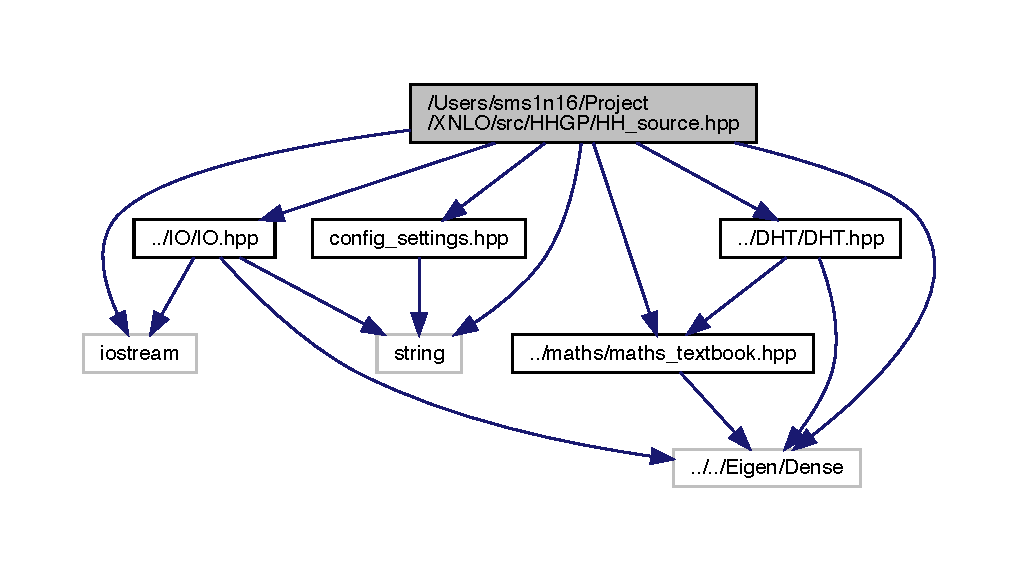
\includegraphics[width=350pt]{_h_h__source_8hpp__incl}
\end{center}
\end{figure}
This graph shows which files directly or indirectly include this file\+:
\nopagebreak
\begin{figure}[H]
\begin{center}
\leavevmode
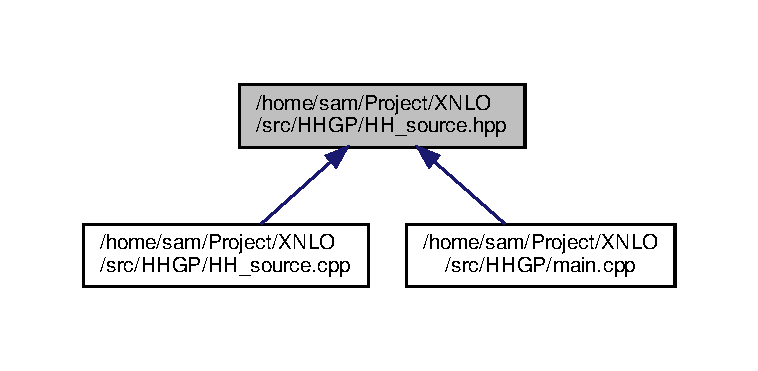
\includegraphics[width=350pt]{_h_h__source_8hpp__dep__incl}
\end{center}
\end{figure}
\subsection*{Classes}
\begin{DoxyCompactItemize}
\item 
class \mbox{\hyperlink{class_h_h__source}{H\+H\+\_\+source}}
\end{DoxyCompactItemize}

\hypertarget{_h_h_g_p_8cpp}{}\section{/home/sam/\+Project/\+X\+N\+L\+O/\+H\+H\+G\+P/src/\+H\+H\+GP.cpp File Reference}
\label{_h_h_g_p_8cpp}\index{/home/sam/\+Project/\+X\+N\+L\+O/\+H\+H\+G\+P/src/\+H\+H\+G\+P.\+cpp@{/home/sam/\+Project/\+X\+N\+L\+O/\+H\+H\+G\+P/src/\+H\+H\+G\+P.\+cpp}}
{\ttfamily \#include $<$iostream$>$}\newline
{\ttfamily \#include $<$string$>$}\newline
{\ttfamily \#include \char`\"{}../../\+Eigen/\+Dense\char`\"{}}\newline
{\ttfamily \#include \char`\"{}H\+H\+G\+P.\+hpp\char`\"{}}\newline
{\ttfamily \#include \char`\"{}config\+\_\+settings.\+hpp\char`\"{}}\newline
{\ttfamily \#include \char`\"{}../../src/maths\+\_\+textbook.\+hpp\char`\"{}}\newline
{\ttfamily \#include \char`\"{}../../src/keldysh\+\_\+gas.\+hpp\char`\"{}}\newline
{\ttfamily \#include \char`\"{}../../src/\+D\+H\+T.\+hpp\char`\"{}}\newline
{\ttfamily \#include \char`\"{}../../src/grid\+\_\+rkr.\+hpp\char`\"{}}\newline
{\ttfamily \#include \char`\"{}propagation.\+hpp\char`\"{}}\newline
{\ttfamily \#include \char`\"{}../../src/\+I\+O.\+hpp\char`\"{}}\newline
Include dependency graph for H\+H\+G\+P.\+cpp\+:
\nopagebreak
\begin{figure}[H]
\begin{center}
\leavevmode
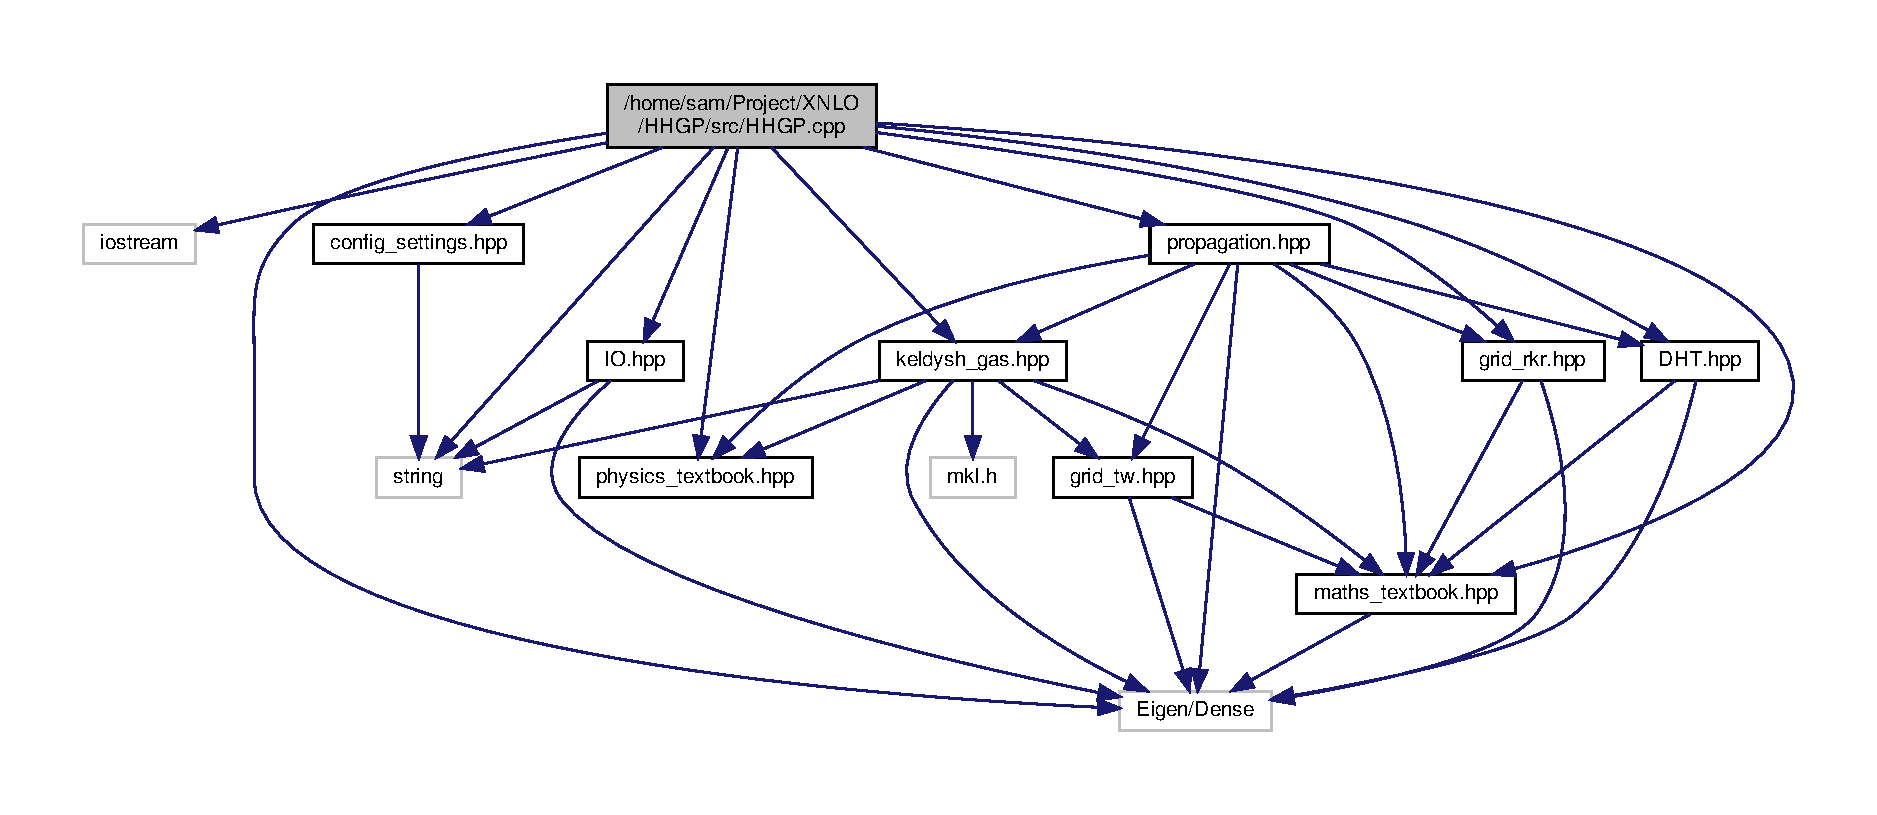
\includegraphics[width=350pt]{_h_h_g_p_8cpp__incl}
\end{center}
\end{figure}

\hypertarget{_h_h_g_p_8hpp}{}\section{/home/sam/\+Project/\+X\+N\+L\+O/src/\+H\+H\+G\+P/\+H\+H\+GP.hpp File Reference}
\label{_h_h_g_p_8hpp}\index{/home/sam/\+Project/\+X\+N\+L\+O/src/\+H\+H\+G\+P/\+H\+H\+G\+P.\+hpp@{/home/sam/\+Project/\+X\+N\+L\+O/src/\+H\+H\+G\+P/\+H\+H\+G\+P.\+hpp}}
{\ttfamily \#include \char`\"{}../../\+Eigen/\+Dense\char`\"{}}\newline
{\ttfamily \#include \char`\"{}config\+\_\+settings.\+hpp\char`\"{}}\newline
{\ttfamily \#include \char`\"{}../maths/maths\+\_\+textbook.\+hpp\char`\"{}}\newline
{\ttfamily \#include \char`\"{}../physics/physics\+\_\+textbook.\+hpp\char`\"{}}\newline
{\ttfamily \#include \char`\"{}../gas/keldysh\+\_\+gas.\+hpp\char`\"{}}\newline
{\ttfamily \#include \char`\"{}../\+D\+H\+T/\+D\+H\+T.\+hpp\char`\"{}}\newline
{\ttfamily \#include \char`\"{}../grid/grid\+\_\+rkr.\+hpp\char`\"{}}\newline
{\ttfamily \#include \char`\"{}propagation.\+hpp\char`\"{}}\newline
{\ttfamily \#include \char`\"{}../\+I\+O/\+I\+O.\+hpp\char`\"{}}\newline
Include dependency graph for H\+H\+G\+P.\+hpp\+:\nopagebreak
\begin{figure}[H]
\begin{center}
\leavevmode
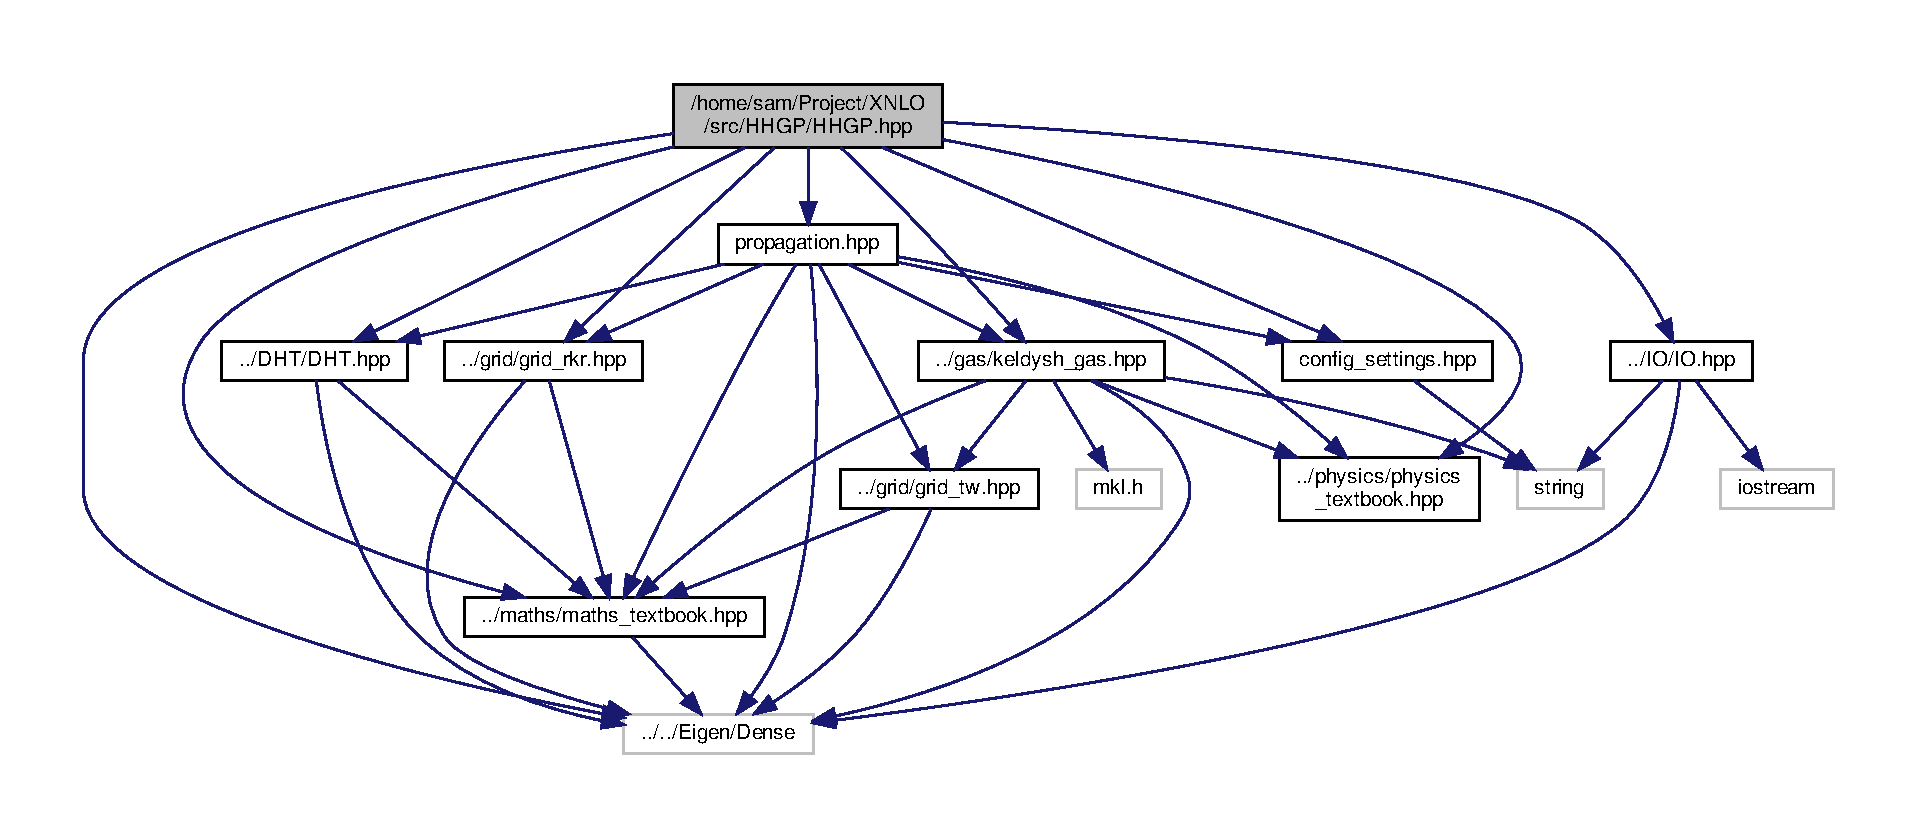
\includegraphics[width=350pt]{_h_h_g_p_8hpp__incl}
\end{center}
\end{figure}
This graph shows which files directly or indirectly include this file\+:\nopagebreak
\begin{figure}[H]
\begin{center}
\leavevmode
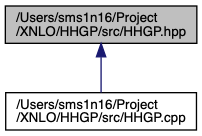
\includegraphics[width=209pt]{_h_h_g_p_8hpp__dep__incl}
\end{center}
\end{figure}
\subsection*{Classes}
\begin{DoxyCompactItemize}
\item 
class \hyperlink{class_h_h_g_p}{H\+H\+GP}
\end{DoxyCompactItemize}

\hypertarget{main_8cpp}{}\section{/home/sam/\+Project/\+X\+N\+L\+O/src/\+H\+H\+G\+P/main.cpp File Reference}
\label{main_8cpp}\index{/home/sam/Project/XNLO/src/HHGP/main.cpp@{/home/sam/Project/XNLO/src/HHGP/main.cpp}}
{\ttfamily \#include $<$iostream$>$}\newline
{\ttfamily \#include $<$string$>$}\newline
{\ttfamily \#include \char`\"{}../../\+Eigen/\+Dense\char`\"{}}\newline
{\ttfamily \#include \char`\"{}config\+\_\+settings.\+hpp\char`\"{}}\newline
{\ttfamily \#include \char`\"{}../maths/maths\+\_\+textbook.\+hpp\char`\"{}}\newline
{\ttfamily \#include \char`\"{}../physics/physics\+\_\+textbook.\+hpp\char`\"{}}\newline
{\ttfamily \#include \char`\"{}H\+H\+\_\+source.\+hpp\char`\"{}}\newline
{\ttfamily \#include \char`\"{}../gas/keldysh\+\_\+gas.\+hpp\char`\"{}}\newline
{\ttfamily \#include \char`\"{}../\+D\+H\+T/\+D\+H\+T.\+hpp\char`\"{}}\newline
{\ttfamily \#include \char`\"{}../grid/grid\+\_\+rkr.\+hpp\char`\"{}}\newline
{\ttfamily \#include \char`\"{}propagation.\+hpp\char`\"{}}\newline
{\ttfamily \#include \char`\"{}../\+I\+O/\+I\+O.\+hpp\char`\"{}}\newline
Include dependency graph for main.\+cpp\+:\nopagebreak
\begin{figure}[H]
\begin{center}
\leavevmode
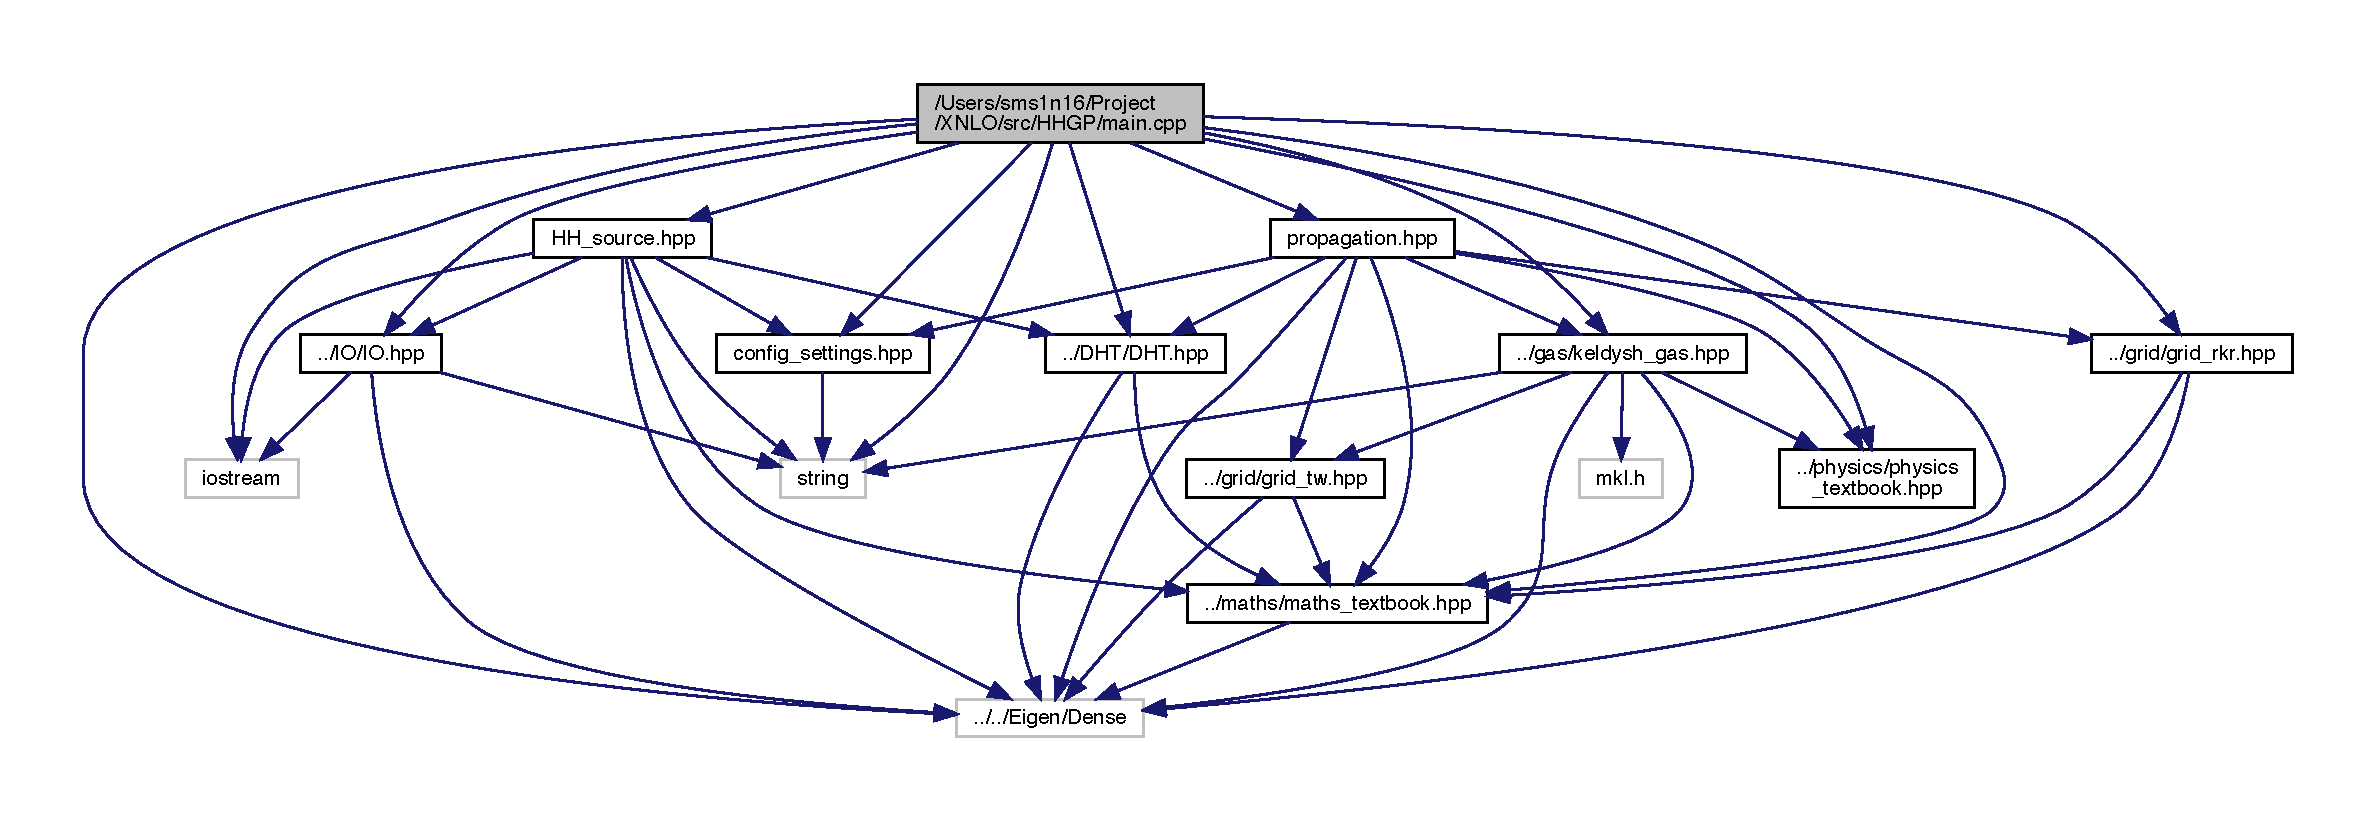
\includegraphics[width=350pt]{main_8cpp__incl}
\end{center}
\end{figure}
\subsection*{Functions}
\begin{DoxyCompactItemize}
\item 
int \mbox{\hyperlink{main_8cpp_a3c04138a5bfe5d72780bb7e82a18e627}{main}} (int argc, char $\ast$$\ast$argv)
\end{DoxyCompactItemize}


\subsection{Function Documentation}
\mbox{\Hypertarget{main_8cpp_a3c04138a5bfe5d72780bb7e82a18e627}\label{main_8cpp_a3c04138a5bfe5d72780bb7e82a18e627}} 
\index{main.cpp@{main.cpp}!main@{main}}
\index{main@{main}!main.cpp@{main.cpp}}
\subsubsection{\texorpdfstring{main()}{main()}}
{\footnotesize\ttfamily int main (\begin{DoxyParamCaption}\item[{int}]{argc,  }\item[{char $\ast$$\ast$}]{argv }\end{DoxyParamCaption})}

2.\+0; 
\hypertarget{propagation_8cpp}{}\section{/home/sam/\+Project/\+X\+N\+L\+O/\+H\+H\+G\+P/src/propagation.cpp File Reference}
\label{propagation_8cpp}\index{/home/sam/\+Project/\+X\+N\+L\+O/\+H\+H\+G\+P/src/propagation.\+cpp@{/home/sam/\+Project/\+X\+N\+L\+O/\+H\+H\+G\+P/src/propagation.\+cpp}}
{\ttfamily \#include \char`\"{}propagation.\+hpp\char`\"{}}\newline
{\ttfamily \#include \char`\"{}../../src/keldysh\+\_\+gas.\+hpp\char`\"{}}\newline
{\ttfamily \#include \char`\"{}../../src/grid\+\_\+rkr.\+hpp\char`\"{}}\newline
{\ttfamily \#include \char`\"{}../../src/grid\+\_\+tw.\+hpp\char`\"{}}\newline
{\ttfamily \#include \char`\"{}../../src/\+D\+H\+T.\+hpp\char`\"{}}\newline
{\ttfamily \#include \char`\"{}../../src/physics\+\_\+textbook.\+hpp\char`\"{}}\newline
{\ttfamily \#include \char`\"{}../../src/maths\+\_\+textbook.\+hpp\char`\"{}}\newline
{\ttfamily \#include \char`\"{}Eigen/\+Dense\char`\"{}}\newline
{\ttfamily \#include $<$iostream$>$}\newline
{\ttfamily \#include \char`\"{}../../src/\+I\+O.\+hpp\char`\"{}}\newline
{\ttfamily \#include $<$complex$>$}\newline
Include dependency graph for propagation.\+cpp\+:
\nopagebreak
\begin{figure}[H]
\begin{center}
\leavevmode
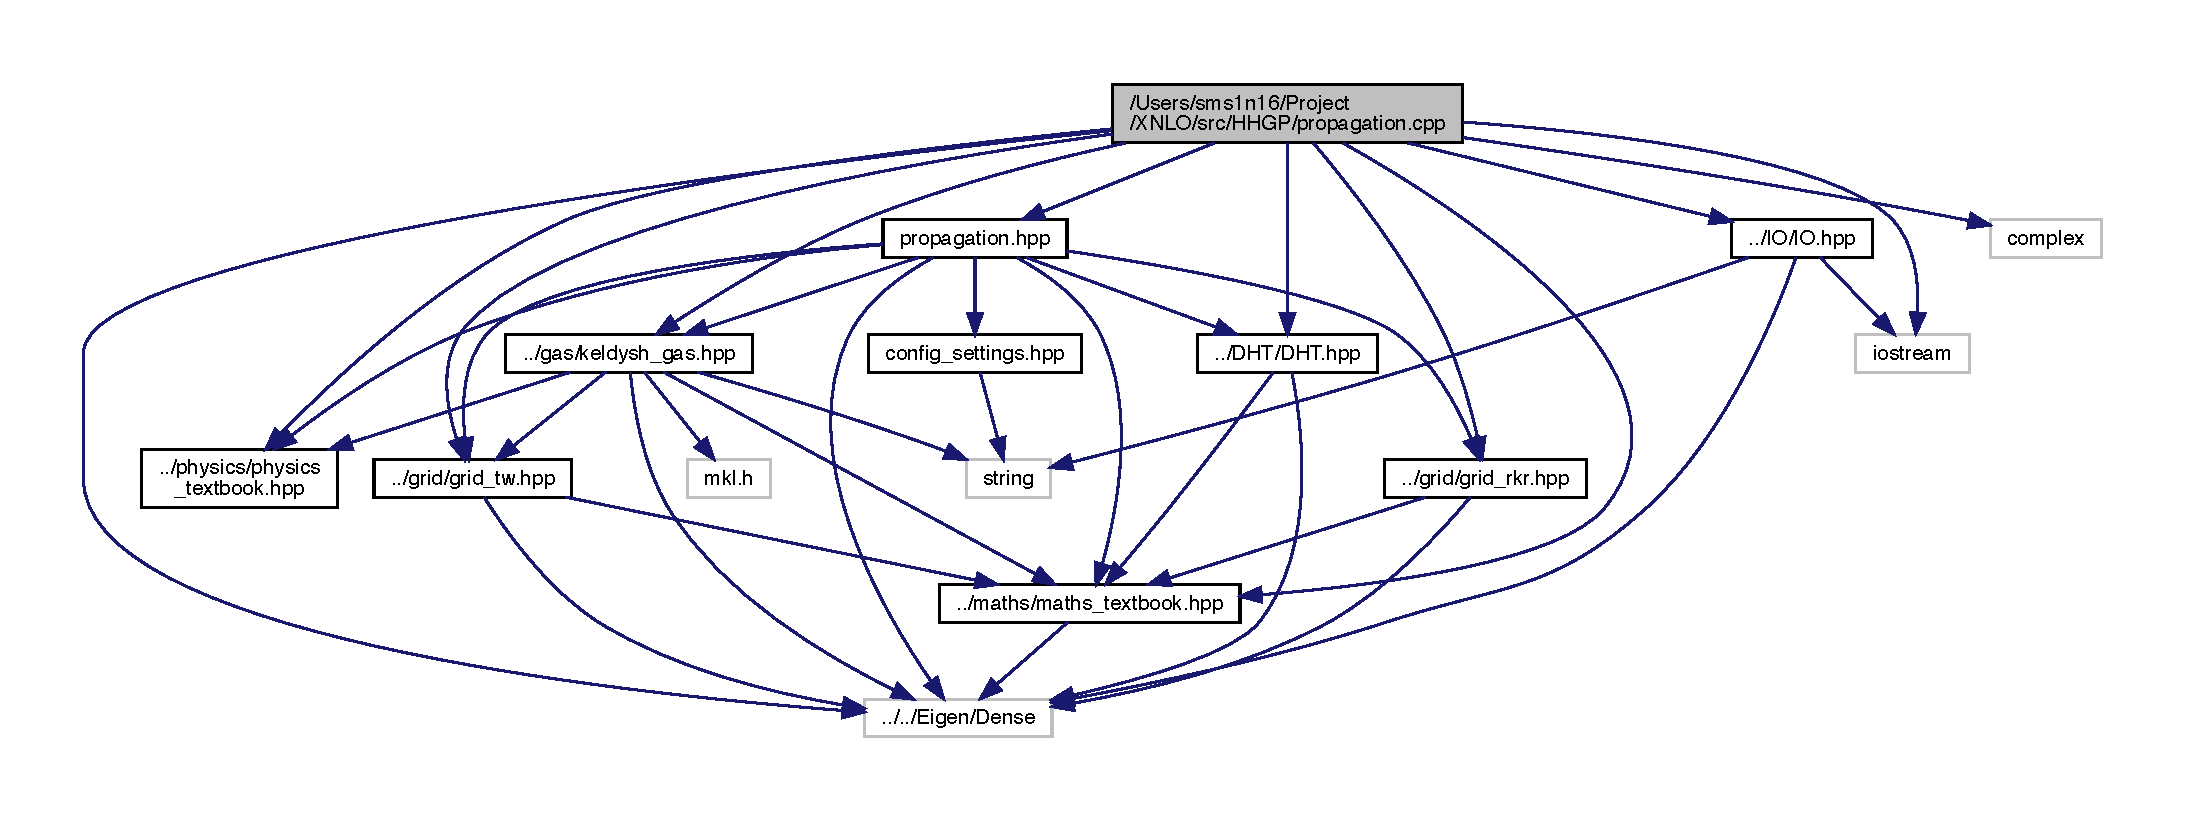
\includegraphics[width=350pt]{propagation_8cpp__incl}
\end{center}
\end{figure}

\hypertarget{propagation_8hpp}{}\section{/home/sam/\+Project/\+X\+N\+L\+O/src/\+H\+H\+G\+P/propagation.hpp File Reference}
\label{propagation_8hpp}\index{/home/sam/\+Project/\+X\+N\+L\+O/src/\+H\+H\+G\+P/propagation.\+hpp@{/home/sam/\+Project/\+X\+N\+L\+O/src/\+H\+H\+G\+P/propagation.\+hpp}}
{\ttfamily \#include \char`\"{}config\+\_\+settings.\+hpp\char`\"{}}\newline
{\ttfamily \#include \char`\"{}../gas/keldysh\+\_\+gas.\+hpp\char`\"{}}\newline
{\ttfamily \#include \char`\"{}../physics/physics\+\_\+textbook.\+hpp\char`\"{}}\newline
{\ttfamily \#include \char`\"{}../maths/maths\+\_\+textbook.\+hpp\char`\"{}}\newline
{\ttfamily \#include \char`\"{}../grid/grid\+\_\+rkr.\+hpp\char`\"{}}\newline
{\ttfamily \#include \char`\"{}../grid/grid\+\_\+tw.\+hpp\char`\"{}}\newline
{\ttfamily \#include \char`\"{}../\+D\+H\+T/\+D\+H\+T.\+hpp\char`\"{}}\newline
{\ttfamily \#include \char`\"{}../../\+Eigen/\+Dense\char`\"{}}\newline
Include dependency graph for propagation.\+hpp\+:\nopagebreak
\begin{figure}[H]
\begin{center}
\leavevmode
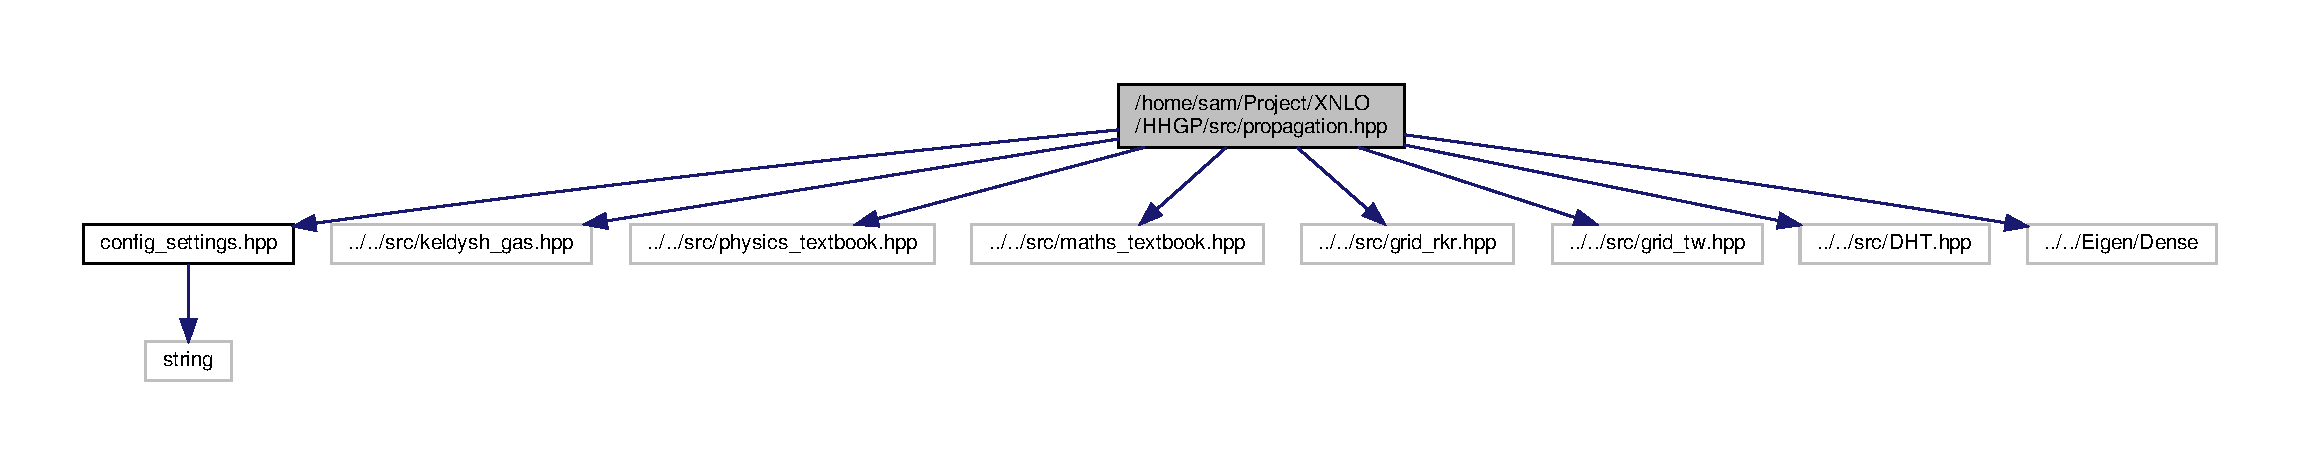
\includegraphics[width=350pt]{propagation_8hpp__incl}
\end{center}
\end{figure}
This graph shows which files directly or indirectly include this file\+:\nopagebreak
\begin{figure}[H]
\begin{center}
\leavevmode
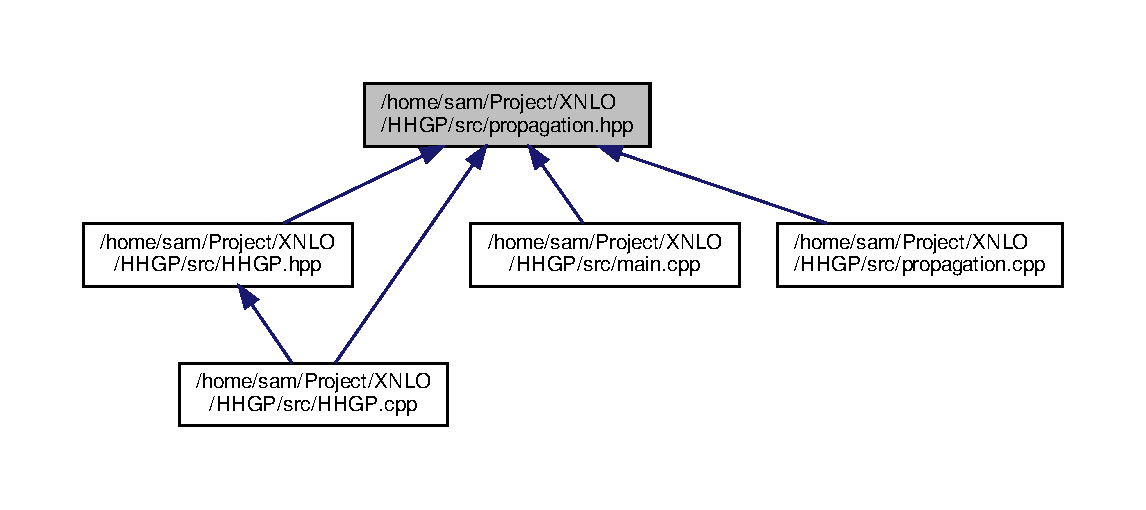
\includegraphics[width=350pt]{propagation_8hpp__dep__incl}
\end{center}
\end{figure}
\subsection*{Classes}
\begin{DoxyCompactItemize}
\item 
class \hyperlink{classpropagation}{propagation}
\end{DoxyCompactItemize}

\hypertarget{_i_o_8cpp}{}\section{/home/sam/\+Project/\+X\+N\+L\+O/\+H\+H\+G\+P/src/\+IO.cpp File Reference}
\label{_i_o_8cpp}\index{/home/sam/\+Project/\+X\+N\+L\+O/\+H\+H\+G\+P/src/\+I\+O.\+cpp@{/home/sam/\+Project/\+X\+N\+L\+O/\+H\+H\+G\+P/src/\+I\+O.\+cpp}}
{\ttfamily \#include \char`\"{}I\+O.\+hpp\char`\"{}}\newline
{\ttfamily \#include \char`\"{}Eigen/\+Dense\char`\"{}}\newline
{\ttfamily \#include $<$fstream$>$}\newline
{\ttfamily \#include $<$iostream$>$}\newline
{\ttfamily \#include $<$string$>$}\newline
Include dependency graph for I\+O.\+cpp\+:\nopagebreak
\begin{figure}[H]
\begin{center}
\leavevmode
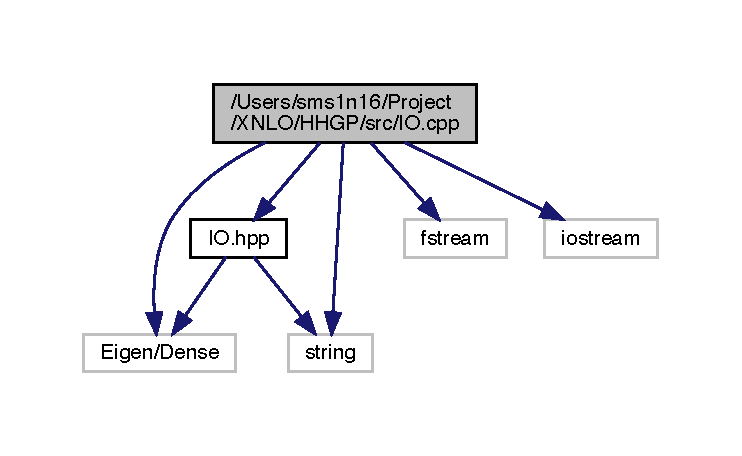
\includegraphics[width=350pt]{_i_o_8cpp__incl}
\end{center}
\end{figure}

\hypertarget{_i_o_8hpp}{}\section{/home/sam/\+Project/\+X\+N\+L\+O/\+H\+H\+G\+P/src/\+IO.hpp File Reference}
\label{_i_o_8hpp}\index{/home/sam/\+Project/\+X\+N\+L\+O/\+H\+H\+G\+P/src/\+I\+O.\+hpp@{/home/sam/\+Project/\+X\+N\+L\+O/\+H\+H\+G\+P/src/\+I\+O.\+hpp}}
{\ttfamily \#include \char`\"{}Eigen/\+Dense\char`\"{}}\newline
{\ttfamily \#include $<$string$>$}\newline
Include dependency graph for I\+O.\+hpp\+:\nopagebreak
\begin{figure}[H]
\begin{center}
\leavevmode
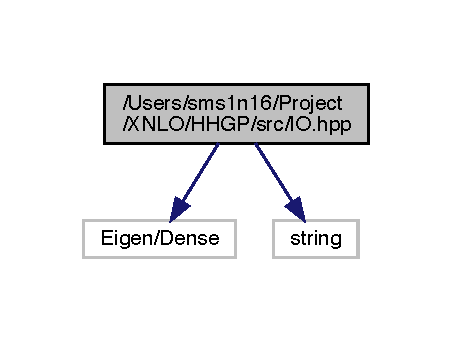
\includegraphics[width=217pt]{_i_o_8hpp__incl}
\end{center}
\end{figure}
This graph shows which files directly or indirectly include this file\+:
\nopagebreak
\begin{figure}[H]
\begin{center}
\leavevmode
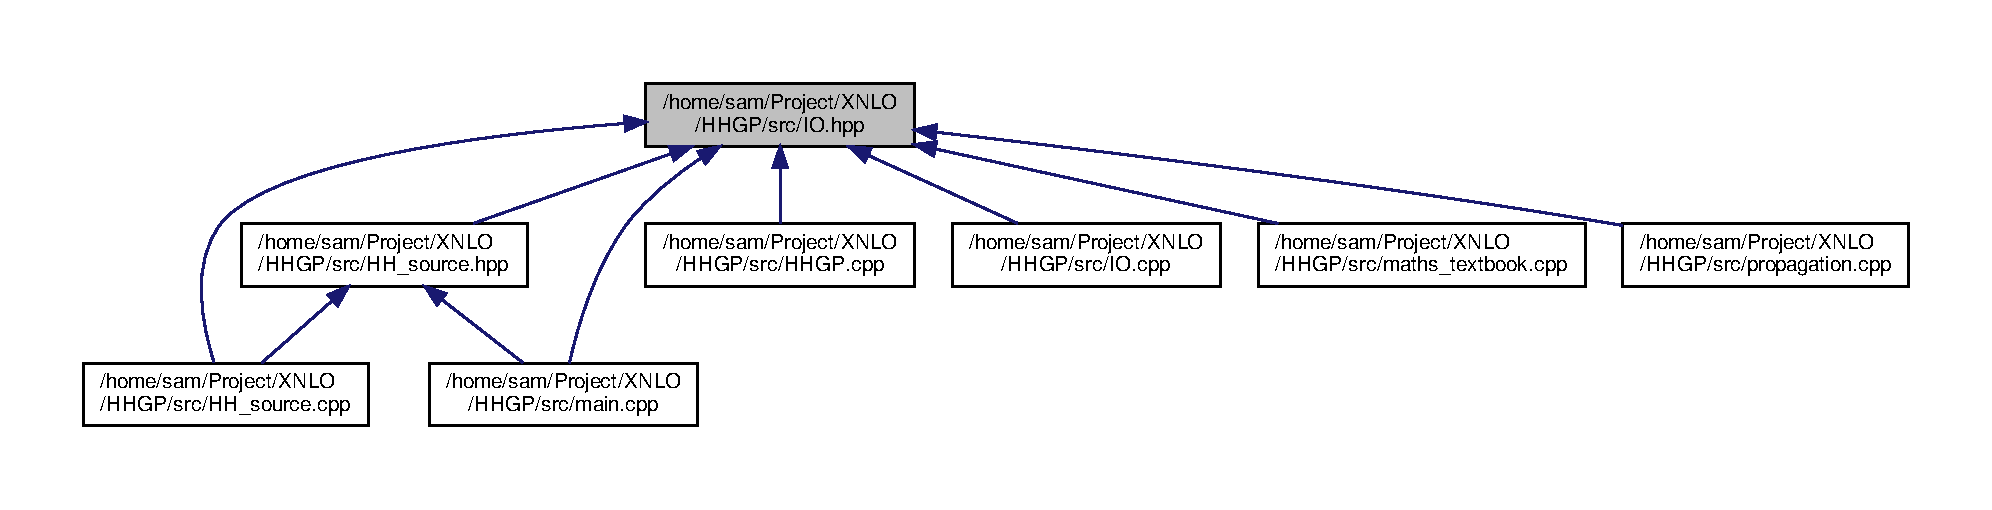
\includegraphics[width=350pt]{_i_o_8hpp__dep__incl}
\end{center}
\end{figure}
\subsection*{Classes}
\begin{DoxyCompactItemize}
\item 
class \hyperlink{class_i_o}{IO}
\end{DoxyCompactItemize}

\hypertarget{maths__textbook_8cpp}{}\section{/home/sam/\+Project/\+X\+N\+L\+O/src/maths/maths\+\_\+textbook.cpp File Reference}
\label{maths__textbook_8cpp}\index{/home/sam/Project/XNLO/src/maths/maths\_textbook.cpp@{/home/sam/Project/XNLO/src/maths/maths\_textbook.cpp}}
{\ttfamily \#include \char`\"{}maths\+\_\+textbook.\+hpp\char`\"{}}\newline
{\ttfamily \#include \char`\"{}../\+I\+O/\+I\+O.\+hpp\char`\"{}}\newline
{\ttfamily \#include $<$cmath$>$}\newline
{\ttfamily \#include \char`\"{}../../\+Eigen/\+Dense\char`\"{}}\newline
{\ttfamily \#include $<$mkl.\+h$>$}\newline
{\ttfamily \#include $<$iostream$>$}\newline
Include dependency graph for maths\+\_\+textbook.\+cpp\+:
\nopagebreak
\begin{figure}[H]
\begin{center}
\leavevmode
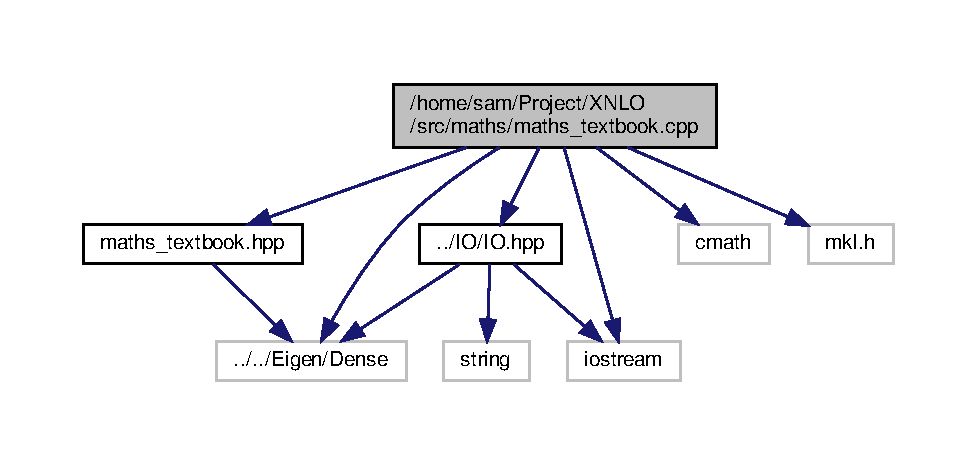
\includegraphics[width=350pt]{maths__textbook_8cpp__incl}
\end{center}
\end{figure}

\hypertarget{maths__textbook_8hpp}{}\section{/home/sam/\+Project/\+X\+N\+L\+O/\+H\+H\+G\+P/src/maths\+\_\+textbook.hpp File Reference}
\label{maths__textbook_8hpp}\index{/home/sam/\+Project/\+X\+N\+L\+O/\+H\+H\+G\+P/src/maths\+\_\+textbook.\+hpp@{/home/sam/\+Project/\+X\+N\+L\+O/\+H\+H\+G\+P/src/maths\+\_\+textbook.\+hpp}}
{\ttfamily \#include \char`\"{}Eigen/\+Dense\char`\"{}}\newline
Include dependency graph for maths\+\_\+textbook.\+hpp\+:\nopagebreak
\begin{figure}[H]
\begin{center}
\leavevmode
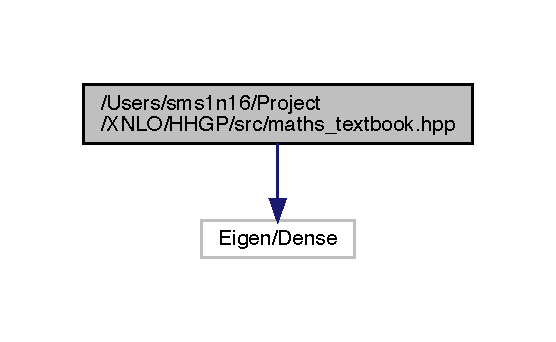
\includegraphics[width=267pt]{maths__textbook_8hpp__incl}
\end{center}
\end{figure}
This graph shows which files directly or indirectly include this file\+:\nopagebreak
\begin{figure}[H]
\begin{center}
\leavevmode
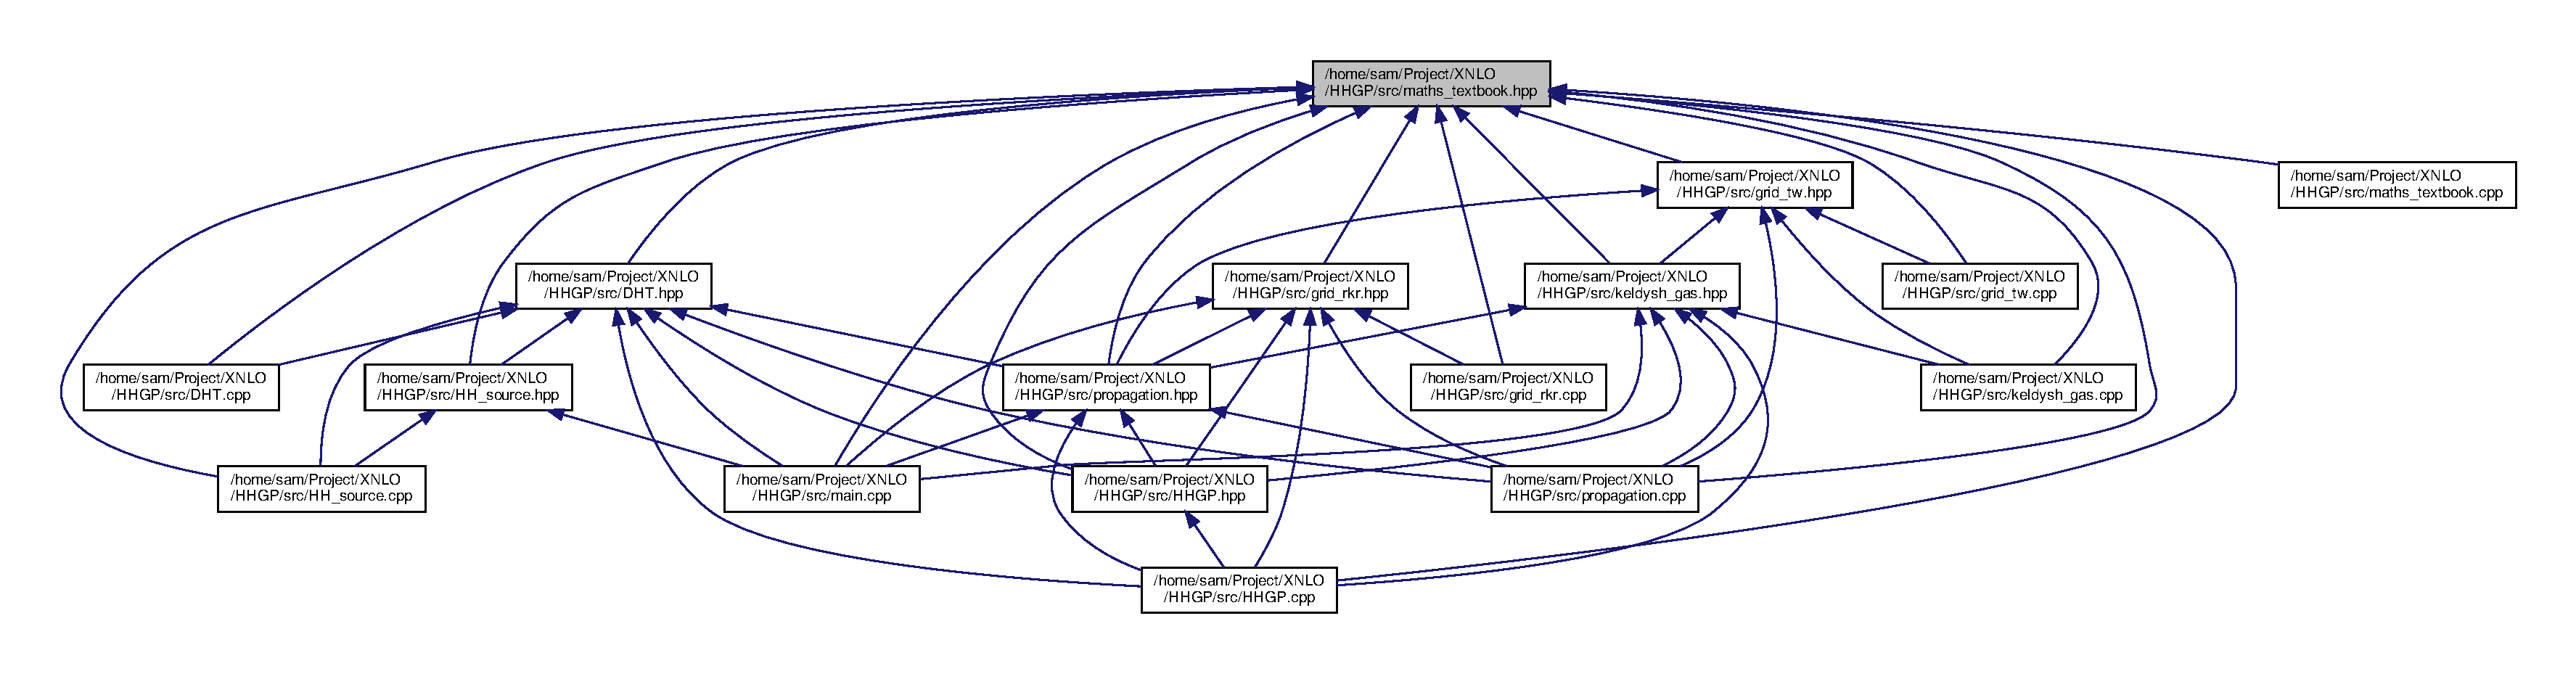
\includegraphics[width=350pt]{maths__textbook_8hpp__dep__incl}
\end{center}
\end{figure}
\subsection*{Classes}
\begin{DoxyCompactItemize}
\item 
class \hyperlink{class_h_h_g_p_1_1maths__textbook}{H\+H\+G\+P\+::maths\+\_\+textbook}
\end{DoxyCompactItemize}
\subsection*{Namespaces}
\begin{DoxyCompactItemize}
\item 
 \hyperlink{namespace_h_h_g_p}{H\+H\+GP}
\end{DoxyCompactItemize}

\hypertarget{physics__textbook_8cpp}{}\section{/home/sam/\+Project/\+X\+N\+L\+O/\+H\+H\+G\+P/src/physics\+\_\+textbook.cpp File Reference}
\label{physics__textbook_8cpp}\index{/home/sam/\+Project/\+X\+N\+L\+O/\+H\+H\+G\+P/src/physics\+\_\+textbook.\+cpp@{/home/sam/\+Project/\+X\+N\+L\+O/\+H\+H\+G\+P/src/physics\+\_\+textbook.\+cpp}}
{\ttfamily \#include \char`\"{}physics\+\_\+textbook.\+hpp\char`\"{}}\newline
Include dependency graph for physics\+\_\+textbook.\+cpp\+:\nopagebreak
\begin{figure}[H]
\begin{center}
\leavevmode
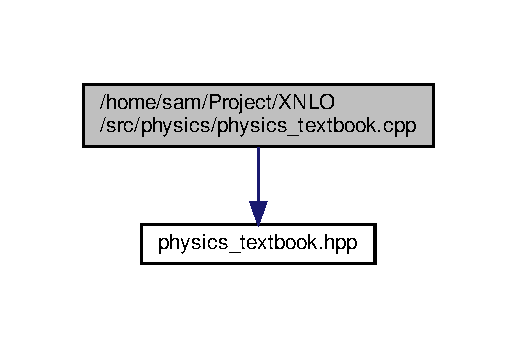
\includegraphics[width=210pt]{physics__textbook_8cpp__incl}
\end{center}
\end{figure}
\subsection*{Namespaces}
\begin{DoxyCompactItemize}
\item 
 \hyperlink{namespace_h_h_g_p}{H\+H\+GP}
\end{DoxyCompactItemize}

\hypertarget{physics__textbook_8hpp}{}\section{/home/sam/\+Project/\+X\+N\+L\+O/\+H\+H\+G\+P/src/physics\+\_\+textbook.hpp File Reference}
\label{physics__textbook_8hpp}\index{/home/sam/\+Project/\+X\+N\+L\+O/\+H\+H\+G\+P/src/physics\+\_\+textbook.\+hpp@{/home/sam/\+Project/\+X\+N\+L\+O/\+H\+H\+G\+P/src/physics\+\_\+textbook.\+hpp}}
This graph shows which files directly or indirectly include this file\+:\nopagebreak
\begin{figure}[H]
\begin{center}
\leavevmode
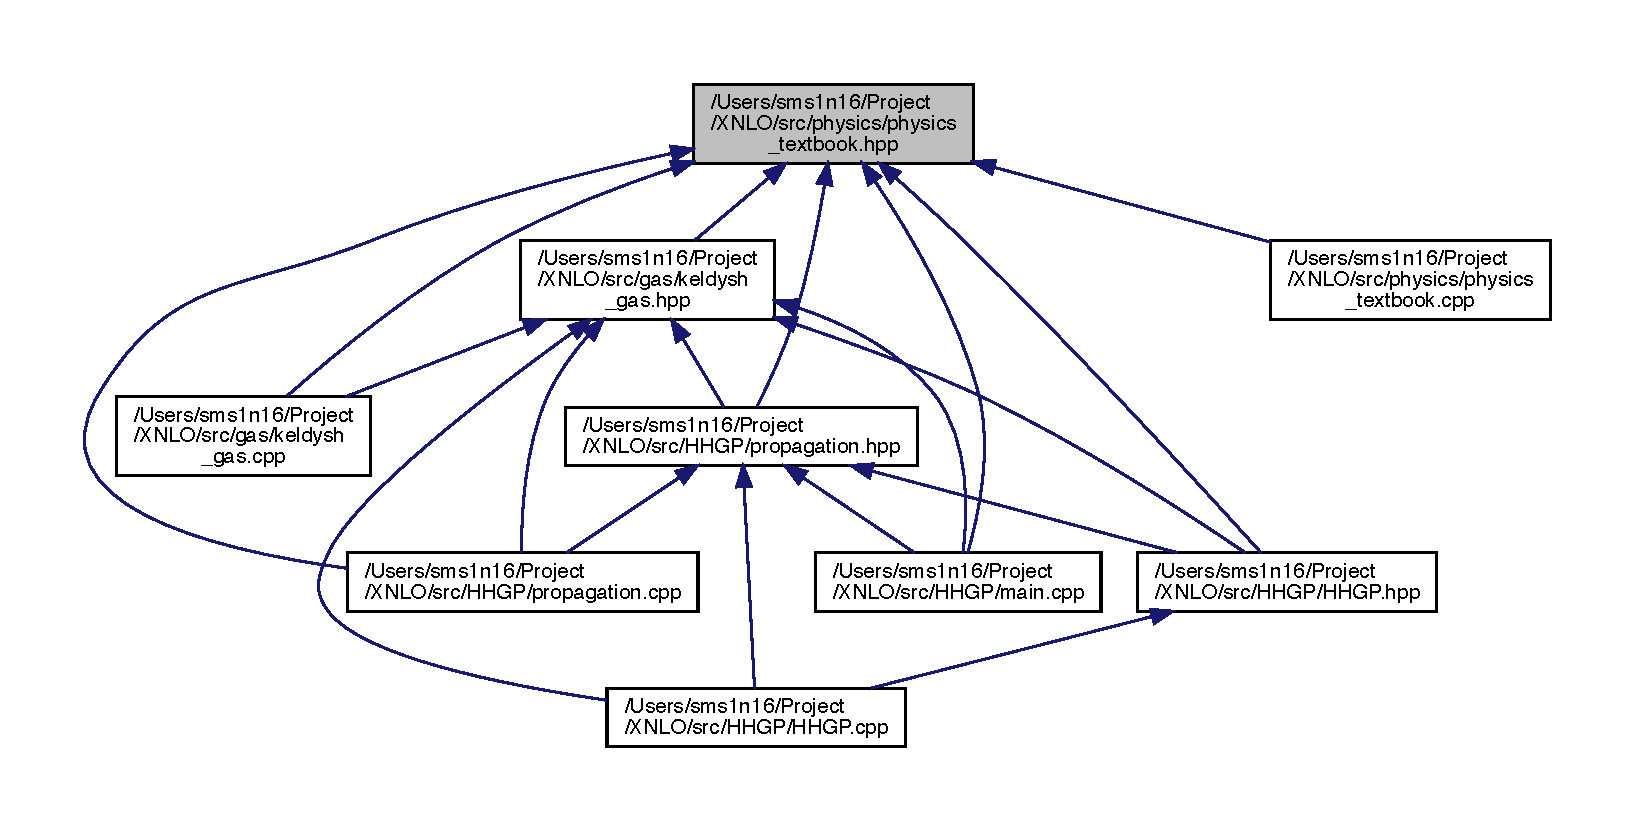
\includegraphics[width=350pt]{physics__textbook_8hpp__dep__incl}
\end{center}
\end{figure}
\subsection*{Classes}
\begin{DoxyCompactItemize}
\item 
class \hyperlink{classphysics__textbook}{physics\+\_\+textbook}
\end{DoxyCompactItemize}

%--- End generated contents ---

% Index
\backmatter
\newpage
\phantomsection
\clearemptydoublepage
\addcontentsline{toc}{chapter}{Index}
\printindex

\end{document}
